\documentclass[a4paper]{book}
\usepackage{makeidx}
\usepackage{natbib}
\usepackage{graphicx}
\usepackage{multicol}
\usepackage{float}
\usepackage{listings}
\usepackage{color}
\usepackage{ifthen}
\usepackage[table]{xcolor}
\usepackage{textcomp}
\usepackage{alltt}
\usepackage{ifpdf}
\ifpdf
\usepackage[pdftex,
            pagebackref=true,
            colorlinks=true,
            linkcolor=blue,
            unicode
           ]{hyperref}
\else
\usepackage[ps2pdf,
            pagebackref=true,
            colorlinks=true,
            linkcolor=blue,
            unicode
           ]{hyperref}
\usepackage{pspicture}
\fi
\usepackage[utf8]{inputenc}
\usepackage{polski}
\usepackage[T1]{fontenc}

\usepackage{mathptmx}
\usepackage[scaled=.90]{helvet}
\usepackage{courier}
\usepackage{sectsty}
\usepackage[titles]{tocloft}
\usepackage{doxygen}
\lstset{language=C++,inputencoding=utf8,basicstyle=\footnotesize,breaklines=true,breakatwhitespace=true,tabsize=8,numbers=left }
\makeindex
\setcounter{tocdepth}{3}
\renewcommand{\footrulewidth}{0.4pt}
\renewcommand{\familydefault}{\sfdefault}
\hfuzz=15pt
\setlength{\emergencystretch}{15pt}
\hbadness=750
\tolerance=750
\begin{document}
\hypersetup{pageanchor=false,citecolor=blue}
\begin{titlepage}
\vspace*{7cm}
\begin{center}
{\Large \-P\-A\-M\-S\-I -\/ pwilkosz \\[1ex]\large 1.\-0 }\\
\vspace*{1cm}
{\large \-Wygenerowano przez Doxygen 1.7.6.1}\\
\vspace*{0.5cm}
{\small Sun Apr 13 2014 23:41:23}\\
\end{center}
\end{titlepage}
\clearemptydoublepage
\pagenumbering{roman}
\tableofcontents
\clearemptydoublepage
\pagenumbering{arabic}
\hypersetup{pageanchor=true,citecolor=blue}
\chapter{\-Indeks klas}
\section{\-Hierarchia klas}
\-Ta lista dziedziczenia posortowana jest z grubsza, choć nie całkowicie, alfabetycznie\-:\begin{DoxyCompactList}
\item \contentsline{section}{algorytm}{\pageref{classalgorytm}}{}
\begin{DoxyCompactList}
\item \contentsline{section}{h\-\_\-sort}{\pageref{classh__sort}}{}
\item \contentsline{section}{kolejka\-\_\-lista}{\pageref{classkolejka__lista}}{}
\item \contentsline{section}{kolejka\-\_\-tablica}{\pageref{classkolejka__tablica}}{}
\item \contentsline{section}{m\-\_\-sort}{\pageref{classm__sort}}{}
\item \contentsline{section}{mnozenie}{\pageref{classmnozenie}}{}
\item \contentsline{section}{q\-\_\-sort}{\pageref{classq__sort}}{}
\item \contentsline{section}{stos\-\_\-lista}{\pageref{classstos__lista}}{}
\item \contentsline{section}{stos\-\_\-tablica}{\pageref{classstos__tablica}}{}
\end{DoxyCompactList}
\item \contentsline{section}{operacje}{\pageref{classoperacje}}{}
\item \contentsline{section}{queue\-\_\-array$<$ \-T\-Y\-P $>$}{\pageref{classqueue__array}}{}
\item \contentsline{section}{queue\-\_\-list$<$ \-T\-Y\-P $>$}{\pageref{classqueue__list}}{}
\item \contentsline{section}{stack\-\_\-array$<$ \-T\-Y\-P $>$}{\pageref{classstack__array}}{}
\item \contentsline{section}{stack\-\_\-list$<$ \-T\-Y\-P $>$}{\pageref{classstack__list}}{}
\end{DoxyCompactList}

\chapter{\-Indeks klas}
\section{\-Lista klas}
\-Tutaj znajdują się klasy, struktury, unie i interfejsy wraz z ich krótkimi opisami\-:\begin{DoxyCompactList}
\item\contentsline{section}{\hyperlink{classalgorytm}{algorytm} \\*\-Definicja klasy algorytm \-Jest to klasa bazowa, ktora ma za zadanie wczytac, przetworzyc i porownac dane z plikiem wzorcowym }{\pageref{classalgorytm}}{}
\item\contentsline{section}{\hyperlink{classmnozenie}{mnozenie} \\*\-Modeluje algorytm dokonujacy mnozenia kazdego elementu pliku wejsciowego przez 2 }{\pageref{classmnozenie}}{}
\item\contentsline{section}{\hyperlink{classoperacje}{operacje} \\*\-Klasa modeluje tablice z danymi i metody sluzace do operacji na niej }{\pageref{classoperacje}}{}
\end{DoxyCompactList}

\chapter{\-Indeks plików}
\section{Lista plików}
Tutaj znajduje się lista wszystkich plików z ich krótkimi opisami\-:\begin{DoxyCompactList}
\item\contentsline{section}{\hyperlink{algorytm_8cpp}{algorytm.\-cpp} \\*Plik zawiera definicje metod klas zdefiniowanych w pliku \hyperlink{algorytm_8hh}{algorytm.\-hh} }{\pageref{algorytm_8cpp}}{}
\item\contentsline{section}{\hyperlink{algorytm_8hh}{algorytm.\-hh} \\*Definicja klas wykonujacych operacje na zestawie danych wejsciowych }{\pageref{algorytm_8hh}}{}
\item\contentsline{section}{\hyperlink{drzewo_8hh}{drzewo.\-hh} }{\pageref{drzewo_8hh}}{}
\item\contentsline{section}{\hyperlink{graf_8cpp}{graf.\-cpp} }{\pageref{graf_8cpp}}{}
\item\contentsline{section}{\hyperlink{graf_8hh}{graf.\-hh} }{\pageref{graf_8hh}}{}
\item\contentsline{section}{\hyperlink{hashtab_8hh}{hashtab.\-hh} }{\pageref{hashtab_8hh}}{}
\item\contentsline{section}{\hyperlink{kolejka_8hh}{kolejka.\-hh} \\*Plik zawiera definicje klasy Kolejka Zaimplementowanej na 2 sposoby }{\pageref{kolejka_8hh}}{}
\item\contentsline{section}{\hyperlink{main_8cpp}{main.\-cpp} \\*Plik glowny }{\pageref{main_8cpp}}{}
\item\contentsline{section}{\hyperlink{operacje_8cpp}{operacje.\-cpp} }{\pageref{operacje_8cpp}}{}
\item\contentsline{section}{\hyperlink{operacje_8hh}{operacje.\-hh} }{\pageref{operacje_8hh}}{}
\item\contentsline{section}{\hyperlink{simplex_8cpp}{simplex.\-cpp} }{\pageref{simplex_8cpp}}{}
\item\contentsline{section}{\hyperlink{simplex_8hh}{simplex.\-hh} }{\pageref{simplex_8hh}}{}
\item\contentsline{section}{\hyperlink{statystyki_8cpp}{statystyki.\-cpp} }{\pageref{statystyki_8cpp}}{}
\item\contentsline{section}{\hyperlink{statystyki_8hh}{statystyki.\-hh} \\*Plik zawiera dekalracje funkcji odpowiedzialnych za przeprowadznaie statystyk }{\pageref{statystyki_8hh}}{}
\item\contentsline{section}{\hyperlink{stos_8hh}{stos.\-hh} \\*Plik zawiera definicje klasy {\ttfamily Stos} Zaimplementowana na 2 sposoby }{\pageref{stos_8hh}}{}
\item\contentsline{section}{\hyperlink{str__operacje_8cpp}{str\-\_\-operacje.\-cpp} }{\pageref{str__operacje_8cpp}}{}
\item\contentsline{section}{\hyperlink{str__operacje_8hh}{str\-\_\-operacje.\-hh} }{\pageref{str__operacje_8hh}}{}
\item\contentsline{section}{\hyperlink{tablica__asocjacyjna_8hh}{tablica\-\_\-asocjacyjna.\-hh} }{\pageref{tablica__asocjacyjna_8hh}}{}
\end{DoxyCompactList}

\chapter{\-Dokumentacja klas}
\hypertarget{classalgorytm}{\section{\-Dokumentacja klasy algorytm}
\label{classalgorytm}\index{algorytm@{algorytm}}
}


\-Definicja klasy algorytm \-Jest to klasa bazowa, ktora ma za zadanie wczytac, przetworzyc i porownac plik z plikiem wzorcowym.  




{\ttfamily \#include $<$algorytm.\-hh$>$}



\-Diagram dziedziczenia dla algorytm
\nopagebreak
\begin{figure}[H]
\begin{center}
\leavevmode
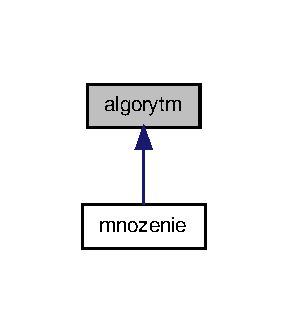
\includegraphics[width=138pt]{classalgorytm__inherit__graph}
\end{center}
\end{figure}
\subsection*{\-Metody publiczne}
\begin{DoxyCompactItemize}
\item 
\hyperlink{classalgorytm_a138ed27849535b192fec3d2e9f6a644f}{algorytm} (const char $\ast$plik1, const char $\ast$plik2)
\begin{DoxyCompactList}\small\item\em konstruktor kopiujacy -\/ przekazuje informacje o nazwach plikow, ktore zapisywane sa do pol klasy \end{DoxyCompactList}\item 
virtual void \hyperlink{classalgorytm_a85ba543fad39e8987bbda4ee698b5fec}{wykonaj} ()
\begin{DoxyCompactList}\small\item\em funkcja dokonuje operacji na pliku wejsciowym \end{DoxyCompactList}\item 
bool \hyperlink{classalgorytm_a167adca6239e12cb5d362fd7c905dde0}{porownaj} ()
\begin{DoxyCompactList}\small\item\em porownuje przetworzony plik z plikiem wzorcowym \end{DoxyCompactList}\item 
int \hyperlink{classalgorytm_acbd9260a0b2055acee485f737b960992}{ile\-\_\-danych} ()
\item 
vector$<$ float $>$ \hyperlink{classalgorytm_a244d9cbf20639faf0b60ae6cdae3c657}{jaki\-\_\-czas} ()
\end{DoxyCompactItemize}
\subsection*{\-Atrybuty publiczne}
\begin{DoxyCompactItemize}
\item 
vector$<$ float $>$ \hyperlink{classalgorytm_aac9e2179e0e956dbe0dc1239ebadb2e4}{czas}
\begin{DoxyCompactList}\small\item\em zawiera wyniki dzialania algorytmu \end{DoxyCompactList}\end{DoxyCompactItemize}
\subsection*{\-Atrybuty chronione}
\begin{DoxyCompactItemize}
\item 
int \hyperlink{classalgorytm_a2778c37f0ec06a30b7d494501c40e91a}{n}
\begin{DoxyCompactList}\small\item\em zawiera informacje o ilosci liczb w pliku \end{DoxyCompactList}\item 
const char $\ast$ \hyperlink{classalgorytm_ab911ca0437df967d0240651855e5a2a3}{plik\-We}
\begin{DoxyCompactList}\small\item\em zawiera nazwe pliku wejsciowego \end{DoxyCompactList}\item 
const char $\ast$ \hyperlink{classalgorytm_a19c2be15efb3e5e34bf177d50b746d93}{plik\-Wz}
\begin{DoxyCompactList}\small\item\em zawiera nazwe pliku wzorcowego \end{DoxyCompactList}\end{DoxyCompactItemize}


\subsection{\-Opis szczegółowy}
\-Definicja klasy algorytm \-Jest to klasa bazowa, ktora ma za zadanie wczytac, przetworzyc i porownac plik z plikiem wzorcowym. 

\-Definicja w linii 32 pliku algorytm.\-hh.



\subsection{\-Dokumentacja konstruktora i destruktora}
\hypertarget{classalgorytm_a138ed27849535b192fec3d2e9f6a644f}{\index{algorytm@{algorytm}!algorytm@{algorytm}}
\index{algorytm@{algorytm}!algorytm@{algorytm}}
\subsubsection[{algorytm}]{\setlength{\rightskip}{0pt plus 5cm}{\bf algorytm\-::algorytm} (
\begin{DoxyParamCaption}
\item[{const char $\ast$}]{plik1, }
\item[{const char $\ast$}]{plik2}
\end{DoxyParamCaption}
)\hspace{0.3cm}{\ttfamily  \mbox{[}inline\mbox{]}}}}\label{classalgorytm_a138ed27849535b192fec3d2e9f6a644f}


konstruktor kopiujacy -\/ przekazuje informacje o nazwach plikow, ktore zapisywane sa do pol klasy 


\begin{DoxyParams}{\-Parametry}
{\em plik1} & -\/ plik wejsciowy \\
\hline
{\em plik2} & -\/ plik wzorcowy \\
\hline
\end{DoxyParams}


\-Definicja w linii 56 pliku algorytm.\-hh.



\subsection{\-Dokumentacja funkcji składowych}
\hypertarget{classalgorytm_acbd9260a0b2055acee485f737b960992}{\index{algorytm@{algorytm}!ile\-\_\-danych@{ile\-\_\-danych}}
\index{ile\-\_\-danych@{ile\-\_\-danych}!algorytm@{algorytm}}
\subsubsection[{ile\-\_\-danych}]{\setlength{\rightskip}{0pt plus 5cm}int {\bf algorytm\-::ile\-\_\-danych} (
\begin{DoxyParamCaption}
{}
\end{DoxyParamCaption}
)}}\label{classalgorytm_acbd9260a0b2055acee485f737b960992}
\begin{DoxyReturn}{\-Zwraca}
ilosc liczb wejsciowych 
\end{DoxyReturn}


\-Definicja w linii 16 pliku algorytm.\-cpp.

\hypertarget{classalgorytm_a244d9cbf20639faf0b60ae6cdae3c657}{\index{algorytm@{algorytm}!jaki\-\_\-czas@{jaki\-\_\-czas}}
\index{jaki\-\_\-czas@{jaki\-\_\-czas}!algorytm@{algorytm}}
\subsubsection[{jaki\-\_\-czas}]{\setlength{\rightskip}{0pt plus 5cm}vector$<$ float $>$ {\bf algorytm\-::jaki\-\_\-czas} (
\begin{DoxyParamCaption}
{}
\end{DoxyParamCaption}
)}}\label{classalgorytm_a244d9cbf20639faf0b60ae6cdae3c657}


\-Definicja w linii 19 pliku algorytm.\-cpp.

\hypertarget{classalgorytm_a167adca6239e12cb5d362fd7c905dde0}{\index{algorytm@{algorytm}!porownaj@{porownaj}}
\index{porownaj@{porownaj}!algorytm@{algorytm}}
\subsubsection[{porownaj}]{\setlength{\rightskip}{0pt plus 5cm}bool {\bf algorytm\-::porownaj} (
\begin{DoxyParamCaption}
{}
\end{DoxyParamCaption}
)}}\label{classalgorytm_a167adca6239e12cb5d362fd7c905dde0}


porownuje przetworzony plik z plikiem wzorcowym 

\begin{DoxyReturn}{\-Zwraca}
true -\/ gdy pliki zgodne false -\/ w przeciwnym przypadku 
\end{DoxyReturn}


\-Definicja w linii 23 pliku algorytm.\-cpp.



\-Oto graf wywoływań tej funkcji\-:
\nopagebreak
\begin{figure}[H]
\begin{center}
\leavevmode
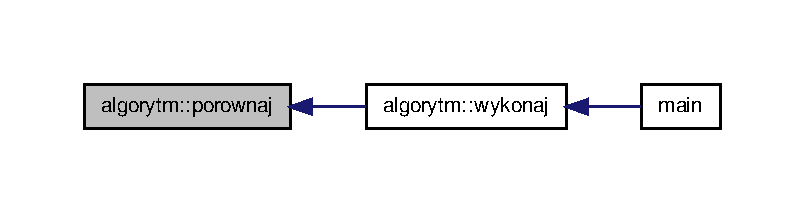
\includegraphics[width=350pt]{classalgorytm_a167adca6239e12cb5d362fd7c905dde0_icgraph}
\end{center}
\end{figure}


\hypertarget{classalgorytm_a85ba543fad39e8987bbda4ee698b5fec}{\index{algorytm@{algorytm}!wykonaj@{wykonaj}}
\index{wykonaj@{wykonaj}!algorytm@{algorytm}}
\subsubsection[{wykonaj}]{\setlength{\rightskip}{0pt plus 5cm}void {\bf algorytm\-::wykonaj} (
\begin{DoxyParamCaption}
{}
\end{DoxyParamCaption}
)\hspace{0.3cm}{\ttfamily  \mbox{[}virtual\mbox{]}}}}\label{classalgorytm_a85ba543fad39e8987bbda4ee698b5fec}


funkcja dokonuje operacji na pliku wejsciowym 



\-Reimplementowana w \hyperlink{classmnozenie_a2c5dc64610bb16af0ef18d142d6af2c0}{mnozenie}.



\-Definicja w linii 7 pliku algorytm.\-cpp.



\subsection{\-Dokumentacja atrybutów składowych}
\hypertarget{classalgorytm_aac9e2179e0e956dbe0dc1239ebadb2e4}{\index{algorytm@{algorytm}!czas@{czas}}
\index{czas@{czas}!algorytm@{algorytm}}
\subsubsection[{czas}]{\setlength{\rightskip}{0pt plus 5cm}vector$<$float$>$ {\bf algorytm\-::czas}}}\label{classalgorytm_aac9e2179e0e956dbe0dc1239ebadb2e4}


zawiera wyniki dzialania algorytmu 



\-Definicja w linii 50 pliku algorytm.\-hh.

\hypertarget{classalgorytm_a2778c37f0ec06a30b7d494501c40e91a}{\index{algorytm@{algorytm}!n@{n}}
\index{n@{n}!algorytm@{algorytm}}
\subsubsection[{n}]{\setlength{\rightskip}{0pt plus 5cm}int {\bf algorytm\-::n}\hspace{0.3cm}{\ttfamily  \mbox{[}protected\mbox{]}}}}\label{classalgorytm_a2778c37f0ec06a30b7d494501c40e91a}


zawiera informacje o ilosci liczb w pliku 



\-Definicja w linii 37 pliku algorytm.\-hh.

\hypertarget{classalgorytm_ab911ca0437df967d0240651855e5a2a3}{\index{algorytm@{algorytm}!plik\-We@{plik\-We}}
\index{plik\-We@{plik\-We}!algorytm@{algorytm}}
\subsubsection[{plik\-We}]{\setlength{\rightskip}{0pt plus 5cm}const char$\ast$ {\bf algorytm\-::plik\-We}\hspace{0.3cm}{\ttfamily  \mbox{[}protected\mbox{]}}}}\label{classalgorytm_ab911ca0437df967d0240651855e5a2a3}


zawiera nazwe pliku wejsciowego 



\-Definicja w linii 41 pliku algorytm.\-hh.

\hypertarget{classalgorytm_a19c2be15efb3e5e34bf177d50b746d93}{\index{algorytm@{algorytm}!plik\-Wz@{plik\-Wz}}
\index{plik\-Wz@{plik\-Wz}!algorytm@{algorytm}}
\subsubsection[{plik\-Wz}]{\setlength{\rightskip}{0pt plus 5cm}const char$\ast$ {\bf algorytm\-::plik\-Wz}\hspace{0.3cm}{\ttfamily  \mbox{[}protected\mbox{]}}}}\label{classalgorytm_a19c2be15efb3e5e34bf177d50b746d93}


zawiera nazwe pliku wzorcowego 



\-Definicja w linii 45 pliku algorytm.\-hh.



\-Dokumentacja dla tej klasy została wygenerowana z plików\-:\begin{DoxyCompactItemize}
\item 
\hyperlink{algorytm_8hh}{algorytm.\-hh}\item 
\hyperlink{algorytm_8cpp}{algorytm.\-cpp}\end{DoxyCompactItemize}

\hypertarget{classbst}{\section{Dokumentacja klasy bst}
\label{classbst}\index{bst@{bst}}
}


Modeluje drzewo binarne przeznaczone do testowania szybkosci wyszukiwnaia.  




{\ttfamily \#include $<$algorytm.\-hh$>$}



Diagram dziedziczenia dla bst\nopagebreak
\begin{figure}[H]
\begin{center}
\leavevmode
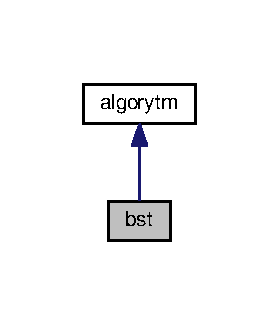
\includegraphics[width=134pt]{classbst__inherit__graph}
\end{center}
\end{figure}


Diagram współpracy dla bst\-:\nopagebreak
\begin{figure}[H]
\begin{center}
\leavevmode
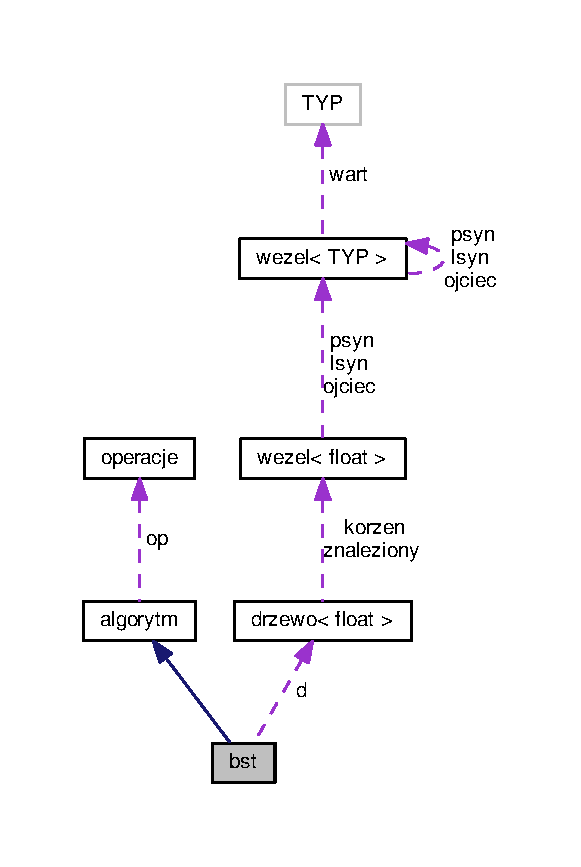
\includegraphics[width=279pt]{classbst__coll__graph}
\end{center}
\end{figure}
\subsection*{Metody publiczne}
\begin{DoxyCompactItemize}
\item 
void \hyperlink{classbst_ac1ed9851250160995112e06c9af324aa}{wczytaj\-\_\-klucze} (ifstream \&plik)
\item 
\hyperlink{classbst_a3f7f0a490dae2027ad55151d40db770a}{bst} (ifstream \&plik1, ifstream \&plik2, ifstream \&plik3, int N, int M)
\item 
\hyperlink{classbst_a4755b663e678f2207dc32caccb5bb18d}{$\sim$bst} ()
\item 
float \hyperlink{classbst_a7991c5cd90a0d350a3150b31aab9401c}{przelicz} ()
\begin{DoxyCompactList}\small\item\em Metoda odpowiada za przetworzenie danych wejsciowych zgodnie z zadanym algorytmem. \end{DoxyCompactList}\end{DoxyCompactItemize}
\subsection*{Atrybuty prywatne}
\begin{DoxyCompactItemize}
\item 
\hyperlink{classdrzewo}{drzewo}$<$ float $>$ \hyperlink{classbst_a50ee6ca023b4ca0484157ccd8716fd37}{d}
\item 
string $\ast$ \hyperlink{classbst_a7e0cb2caf584c2de1d5ba767731c9c3a}{klucze}
\end{DoxyCompactItemize}
\subsection*{Dodatkowe Dziedziczone Składowe}


\subsection{Opis szczegółowy}
Modeluje drzewo binarne przeznaczone do testowania szybkosci wyszukiwnaia. 

Definicja w linii 227 pliku algorytm.\-hh.



\subsection{Dokumentacja konstruktora i destruktora}
\hypertarget{classbst_a3f7f0a490dae2027ad55151d40db770a}{\index{bst@{bst}!bst@{bst}}
\index{bst@{bst}!bst@{bst}}
\subsubsection[{bst}]{\setlength{\rightskip}{0pt plus 5cm}bst\-::bst (
\begin{DoxyParamCaption}
\item[{ifstream \&}]{plik1, }
\item[{ifstream \&}]{plik2, }
\item[{ifstream \&}]{plik3, }
\item[{int}]{N, }
\item[{int}]{M}
\end{DoxyParamCaption}
)\hspace{0.3cm}{\ttfamily [inline]}}}\label{classbst_a3f7f0a490dae2027ad55151d40db770a}


Definicja w linii 232 pliku algorytm.\-hh.

\hypertarget{classbst_a4755b663e678f2207dc32caccb5bb18d}{\index{bst@{bst}!$\sim$bst@{$\sim$bst}}
\index{$\sim$bst@{$\sim$bst}!bst@{bst}}
\subsubsection[{$\sim$bst}]{\setlength{\rightskip}{0pt plus 5cm}bst\-::$\sim$bst (
\begin{DoxyParamCaption}
{}
\end{DoxyParamCaption}
)\hspace{0.3cm}{\ttfamily [inline]}}}\label{classbst_a4755b663e678f2207dc32caccb5bb18d}


Definicja w linii 240 pliku algorytm.\-hh.



\subsection{Dokumentacja funkcji składowych}
\hypertarget{classbst_a7991c5cd90a0d350a3150b31aab9401c}{\index{bst@{bst}!przelicz@{przelicz}}
\index{przelicz@{przelicz}!bst@{bst}}
\subsubsection[{przelicz}]{\setlength{\rightskip}{0pt plus 5cm}float bst\-::przelicz (
\begin{DoxyParamCaption}
{}
\end{DoxyParamCaption}
)\hspace{0.3cm}{\ttfamily [virtual]}}}\label{classbst_a7991c5cd90a0d350a3150b31aab9401c}


Metoda odpowiada za przetworzenie danych wejsciowych zgodnie z zadanym algorytmem. 



Reimplementowana z \hyperlink{classalgorytm_af3f92bf537b1f2e1f93173983e838449}{algorytm}.



Definicja w linii 204 pliku algorytm.\-cpp.



Oto graf wywołań dla tej funkcji\-:\nopagebreak
\begin{figure}[H]
\begin{center}
\leavevmode
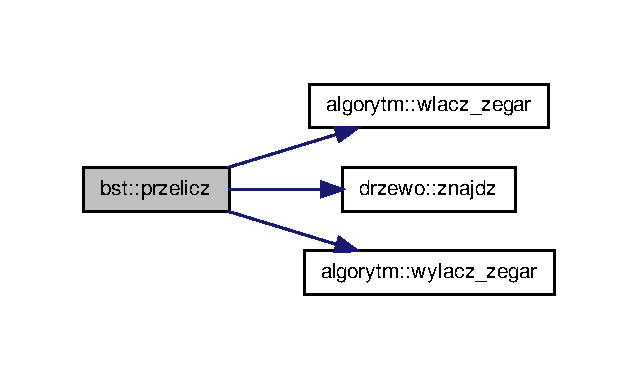
\includegraphics[width=306pt]{classbst_a7991c5cd90a0d350a3150b31aab9401c_cgraph}
\end{center}
\end{figure}


\hypertarget{classbst_ac1ed9851250160995112e06c9af324aa}{\index{bst@{bst}!wczytaj\-\_\-klucze@{wczytaj\-\_\-klucze}}
\index{wczytaj\-\_\-klucze@{wczytaj\-\_\-klucze}!bst@{bst}}
\subsubsection[{wczytaj\-\_\-klucze}]{\setlength{\rightskip}{0pt plus 5cm}void bst\-::wczytaj\-\_\-klucze (
\begin{DoxyParamCaption}
\item[{ifstream \&}]{plik}
\end{DoxyParamCaption}
)}}\label{classbst_ac1ed9851250160995112e06c9af324aa}


Definicja w linii 199 pliku algorytm.\-cpp.



\subsection{Dokumentacja atrybutów składowych}
\hypertarget{classbst_a50ee6ca023b4ca0484157ccd8716fd37}{\index{bst@{bst}!d@{d}}
\index{d@{d}!bst@{bst}}
\subsubsection[{d}]{\setlength{\rightskip}{0pt plus 5cm}{\bf drzewo}$<$float$>$ bst\-::d\hspace{0.3cm}{\ttfamily [private]}}}\label{classbst_a50ee6ca023b4ca0484157ccd8716fd37}


Definicja w linii 228 pliku algorytm.\-hh.

\hypertarget{classbst_a7e0cb2caf584c2de1d5ba767731c9c3a}{\index{bst@{bst}!klucze@{klucze}}
\index{klucze@{klucze}!bst@{bst}}
\subsubsection[{klucze}]{\setlength{\rightskip}{0pt plus 5cm}string$\ast$ bst\-::klucze\hspace{0.3cm}{\ttfamily [private]}}}\label{classbst_a7e0cb2caf584c2de1d5ba767731c9c3a}


Definicja w linii 229 pliku algorytm.\-hh.



Dokumentacja dla tej klasy została wygenerowana z plików\-:\begin{DoxyCompactItemize}
\item 
\hyperlink{algorytm_8hh}{algorytm.\-hh}\item 
\hyperlink{algorytm_8cpp}{algorytm.\-cpp}\end{DoxyCompactItemize}

\hypertarget{classdrzewo}{\section{Dokumentacja szablonu klasy drzewo$<$ T\-Y\-P $>$}
\label{classdrzewo}\index{drzewo$<$ T\-Y\-P $>$@{drzewo$<$ T\-Y\-P $>$}}
}


modeluje binarne drzewo przeszukiwan  




{\ttfamily \#include $<$drzewo.\-hh$>$}

\subsection*{Metody publiczne}
\begin{DoxyCompactItemize}
\item 
\hyperlink{classdrzewo_ad43b2e4e82dc089736b57064865fa449}{drzewo} ()
\begin{DoxyCompactList}\small\item\em konstruktor bezparametryczny \end{DoxyCompactList}\item 
\hyperlink{classdrzewo_abaa93ec27e55b1a58c747f680446ffd4}{drzewo} (string k, T\-Y\-P v)
\begin{DoxyCompactList}\small\item\em konstruktor parametryczny -\/ przypisuje korzeniowi klucz i wartosc \end{DoxyCompactList}\item 
void \hyperlink{classdrzewo_a9c52aa0c3842425ff5900429bbf0c43d}{dodaj\-\_\-wezel} (\hyperlink{classwezel}{wezel}$<$ T\-Y\-P $>$ $\ast$W)
\begin{DoxyCompactList}\small\item\em dodaje wezel do drzewa \end{DoxyCompactList}\item 
void \hyperlink{classdrzewo_a53ccf9b49a62bcb6b5dfab4e48415cc1}{dodaj} (string k, T\-Y\-P v)
\begin{DoxyCompactList}\small\item\em dodaje wezel do drzewa \end{DoxyCompactList}\item 
bool \hyperlink{classdrzewo_ad9d512467919623595126d88bdb60974}{znajdz} (string k)
\begin{DoxyCompactList}\small\item\em szuka wezla o zadanym kluczu \end{DoxyCompactList}\item 
bool \hyperlink{classdrzewo_a2670c642c8edfef4a716c39a3dd626a7}{szukaj} (string k, \hyperlink{classwezel}{wezel}$<$ T\-Y\-P $>$ $\ast$w)
\begin{DoxyCompactList}\small\item\em sprawdza, czy w danym wezle znajduje sie szukany klucz \end{DoxyCompactList}\item 
void \hyperlink{classdrzewo_ad80b0276f6f4ed01fb2b42856e62f101}{usun} (string k)
\begin{DoxyCompactList}\small\item\em usuwa element o kluczu k, jezeli zostanie on znaleizony \end{DoxyCompactList}\item 
void \hyperlink{classdrzewo_a52496982e5ad7f4002d343e3637a68da}{czysc} (\hyperlink{classwezel}{wezel}$<$ T\-Y\-P $>$ $\ast$w)
\begin{DoxyCompactList}\small\item\em rekursywne czyszczenie wezla \end{DoxyCompactList}\item 
void \hyperlink{classdrzewo_a25de98ca343edbc949466d3b6cd5ce9f}{wyczysc} ()
\begin{DoxyCompactList}\small\item\em czysci cale drzewo \end{DoxyCompactList}\end{DoxyCompactItemize}
\subsection*{Atrybuty publiczne}
\begin{DoxyCompactItemize}
\item 
\hyperlink{classwezel}{wezel}$<$ T\-Y\-P $>$ $\ast$ \hyperlink{classdrzewo_a8c5c1104e4e6e327ffe7091e96528bf5}{korzen}
\begin{DoxyCompactList}\small\item\em korzen drzewa \end{DoxyCompactList}\item 
\hyperlink{classwezel}{wezel}$<$ T\-Y\-P $>$ $\ast$ \hyperlink{classdrzewo_a5c5ca950d7ee79f135c50bd33dba3745}{znaleziony}
\begin{DoxyCompactList}\small\item\em znaleziony wezel w drzewie \end{DoxyCompactList}\end{DoxyCompactItemize}


\subsection{Opis szczegółowy}
\subsubsection*{template$<$typename T\-Y\-P$>$class drzewo$<$ T\-Y\-P $>$}

modeluje binarne drzewo przeszukiwan 

Definicja w linii 70 pliku drzewo.\-hh.



\subsection{Dokumentacja konstruktora i destruktora}
\hypertarget{classdrzewo_ad43b2e4e82dc089736b57064865fa449}{\index{drzewo@{drzewo}!drzewo@{drzewo}}
\index{drzewo@{drzewo}!drzewo@{drzewo}}
\subsubsection[{drzewo}]{\setlength{\rightskip}{0pt plus 5cm}template$<$typename T\-Y\-P$>$ {\bf drzewo}$<$ T\-Y\-P $>$\-::{\bf drzewo} (
\begin{DoxyParamCaption}
{}
\end{DoxyParamCaption}
)\hspace{0.3cm}{\ttfamily [inline]}}}\label{classdrzewo_ad43b2e4e82dc089736b57064865fa449}


konstruktor bezparametryczny 



Definicja w linii 77 pliku drzewo.\-hh.

\hypertarget{classdrzewo_abaa93ec27e55b1a58c747f680446ffd4}{\index{drzewo@{drzewo}!drzewo@{drzewo}}
\index{drzewo@{drzewo}!drzewo@{drzewo}}
\subsubsection[{drzewo}]{\setlength{\rightskip}{0pt plus 5cm}template$<$typename T\-Y\-P$>$ {\bf drzewo}$<$ T\-Y\-P $>$\-::{\bf drzewo} (
\begin{DoxyParamCaption}
\item[{string}]{k, }
\item[{T\-Y\-P}]{v}
\end{DoxyParamCaption}
)\hspace{0.3cm}{\ttfamily [inline]}}}\label{classdrzewo_abaa93ec27e55b1a58c747f680446ffd4}


konstruktor parametryczny -\/ przypisuje korzeniowi klucz i wartosc 



Definicja w linii 79 pliku drzewo.\-hh.



\subsection{Dokumentacja funkcji składowych}
\hypertarget{classdrzewo_a52496982e5ad7f4002d343e3637a68da}{\index{drzewo@{drzewo}!czysc@{czysc}}
\index{czysc@{czysc}!drzewo@{drzewo}}
\subsubsection[{czysc}]{\setlength{\rightskip}{0pt plus 5cm}template$<$typename T\-Y\-P$>$ void {\bf drzewo}$<$ T\-Y\-P $>$\-::czysc (
\begin{DoxyParamCaption}
\item[{{\bf wezel}$<$ T\-Y\-P $>$ $\ast$}]{w}
\end{DoxyParamCaption}
)\hspace{0.3cm}{\ttfamily [inline]}}}\label{classdrzewo_a52496982e5ad7f4002d343e3637a68da}


rekursywne czyszczenie wezla 


\begin{DoxyParams}[1]{Parametry}
\mbox{\tt in}  & {\em w} & -\/ czyszczony wezel \\
\hline
\end{DoxyParams}


Definicja w linii 180 pliku drzewo.\-hh.

\hypertarget{classdrzewo_a53ccf9b49a62bcb6b5dfab4e48415cc1}{\index{drzewo@{drzewo}!dodaj@{dodaj}}
\index{dodaj@{dodaj}!drzewo@{drzewo}}
\subsubsection[{dodaj}]{\setlength{\rightskip}{0pt plus 5cm}template$<$typename T\-Y\-P$>$ void {\bf drzewo}$<$ T\-Y\-P $>$\-::dodaj (
\begin{DoxyParamCaption}
\item[{string}]{k, }
\item[{T\-Y\-P}]{v}
\end{DoxyParamCaption}
)\hspace{0.3cm}{\ttfamily [inline]}}}\label{classdrzewo_a53ccf9b49a62bcb6b5dfab4e48415cc1}


dodaje wezel do drzewa 


\begin{DoxyParams}[1]{Parametry}
\mbox{\tt in}  & {\em k} & -\/ klucz wezla \\
\hline
\mbox{\tt in}  & {\em v} & = wartosc wezla \\
\hline
\end{DoxyParams}


Definicja w linii 91 pliku drzewo.\-hh.

\hypertarget{classdrzewo_a9c52aa0c3842425ff5900429bbf0c43d}{\index{drzewo@{drzewo}!dodaj\-\_\-wezel@{dodaj\-\_\-wezel}}
\index{dodaj\-\_\-wezel@{dodaj\-\_\-wezel}!drzewo@{drzewo}}
\subsubsection[{dodaj\-\_\-wezel}]{\setlength{\rightskip}{0pt plus 5cm}template$<$typename T\-Y\-P$>$ void {\bf drzewo}$<$ T\-Y\-P $>$\-::dodaj\-\_\-wezel (
\begin{DoxyParamCaption}
\item[{{\bf wezel}$<$ T\-Y\-P $>$ $\ast$}]{W}
\end{DoxyParamCaption}
)\hspace{0.3cm}{\ttfamily [inline]}}}\label{classdrzewo_a9c52aa0c3842425ff5900429bbf0c43d}


dodaje wezel do drzewa 


\begin{DoxyParams}[1]{Parametry}
\mbox{\tt in}  & {\em W} & -\/ utworzony uprzednio wezel \\
\hline
\end{DoxyParams}


Definicja w linii 83 pliku drzewo.\-hh.

\hypertarget{classdrzewo_a2670c642c8edfef4a716c39a3dd626a7}{\index{drzewo@{drzewo}!szukaj@{szukaj}}
\index{szukaj@{szukaj}!drzewo@{drzewo}}
\subsubsection[{szukaj}]{\setlength{\rightskip}{0pt plus 5cm}template$<$typename T\-Y\-P$>$ bool {\bf drzewo}$<$ T\-Y\-P $>$\-::szukaj (
\begin{DoxyParamCaption}
\item[{string}]{k, }
\item[{{\bf wezel}$<$ T\-Y\-P $>$ $\ast$}]{w}
\end{DoxyParamCaption}
)\hspace{0.3cm}{\ttfamily [inline]}}}\label{classdrzewo_a2670c642c8edfef4a716c39a3dd626a7}


sprawdza, czy w danym wezle znajduje sie szukany klucz 


\begin{DoxyParams}[1]{Parametry}
\mbox{\tt in}  & {\em k} & -\/ klucz \\
\hline
\mbox{\tt in}  & {\em w} & -\/ wezel, w ktorym sprawdzany jest klucz \\
\hline
\end{DoxyParams}
\begin{DoxyReturn}{Zwraca}
true, gdy znaleziono, false w przeciwnym przypadku 
\end{DoxyReturn}


Definicja w linii 109 pliku drzewo.\-hh.

\hypertarget{classdrzewo_ad80b0276f6f4ed01fb2b42856e62f101}{\index{drzewo@{drzewo}!usun@{usun}}
\index{usun@{usun}!drzewo@{drzewo}}
\subsubsection[{usun}]{\setlength{\rightskip}{0pt plus 5cm}template$<$typename T\-Y\-P$>$ void {\bf drzewo}$<$ T\-Y\-P $>$\-::usun (
\begin{DoxyParamCaption}
\item[{string}]{k}
\end{DoxyParamCaption}
)\hspace{0.3cm}{\ttfamily [inline]}}}\label{classdrzewo_ad80b0276f6f4ed01fb2b42856e62f101}


usuwa element o kluczu k, jezeli zostanie on znaleizony 


\begin{DoxyParams}[1]{Parametry}
\mbox{\tt in}  & {\em k} & -\/ klucz wezla, ktory nalezy usunac \\
\hline
\end{DoxyParams}


Definicja w linii 124 pliku drzewo.\-hh.

\hypertarget{classdrzewo_a25de98ca343edbc949466d3b6cd5ce9f}{\index{drzewo@{drzewo}!wyczysc@{wyczysc}}
\index{wyczysc@{wyczysc}!drzewo@{drzewo}}
\subsubsection[{wyczysc}]{\setlength{\rightskip}{0pt plus 5cm}template$<$typename T\-Y\-P$>$ void {\bf drzewo}$<$ T\-Y\-P $>$\-::wyczysc (
\begin{DoxyParamCaption}
{}
\end{DoxyParamCaption}
)\hspace{0.3cm}{\ttfamily [inline]}}}\label{classdrzewo_a25de98ca343edbc949466d3b6cd5ce9f}


czysci cale drzewo 



Definicja w linii 188 pliku drzewo.\-hh.

\hypertarget{classdrzewo_ad9d512467919623595126d88bdb60974}{\index{drzewo@{drzewo}!znajdz@{znajdz}}
\index{znajdz@{znajdz}!drzewo@{drzewo}}
\subsubsection[{znajdz}]{\setlength{\rightskip}{0pt plus 5cm}template$<$typename T\-Y\-P$>$ bool {\bf drzewo}$<$ T\-Y\-P $>$\-::znajdz (
\begin{DoxyParamCaption}
\item[{string}]{k}
\end{DoxyParamCaption}
)\hspace{0.3cm}{\ttfamily [inline]}}}\label{classdrzewo_ad9d512467919623595126d88bdb60974}


szuka wezla o zadanym kluczu 


\begin{DoxyParams}[1]{Parametry}
\mbox{\tt in}  & {\em k} & -\/ klucz \\
\hline
\end{DoxyParams}
\begin{DoxyReturn}{Zwraca}
true, gdy znaleziono, w przeciwnym wypadku zwraca false 
\end{DoxyReturn}


Definicja w linii 100 pliku drzewo.\-hh.



Oto graf wywoływań tej funkcji\-:\nopagebreak
\begin{figure}[H]
\begin{center}
\leavevmode
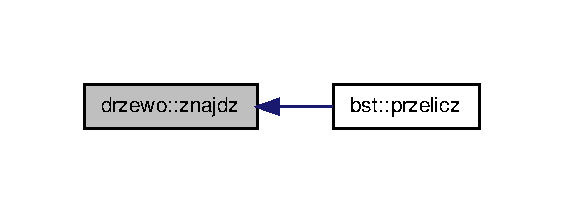
\includegraphics[width=270pt]{classdrzewo_ad9d512467919623595126d88bdb60974_icgraph}
\end{center}
\end{figure}




\subsection{Dokumentacja atrybutów składowych}
\hypertarget{classdrzewo_a8c5c1104e4e6e327ffe7091e96528bf5}{\index{drzewo@{drzewo}!korzen@{korzen}}
\index{korzen@{korzen}!drzewo@{drzewo}}
\subsubsection[{korzen}]{\setlength{\rightskip}{0pt plus 5cm}template$<$typename T\-Y\-P$>$ {\bf wezel}$<$T\-Y\-P$>$$\ast$ {\bf drzewo}$<$ T\-Y\-P $>$\-::korzen}}\label{classdrzewo_a8c5c1104e4e6e327ffe7091e96528bf5}


korzen drzewa 



Definicja w linii 73 pliku drzewo.\-hh.

\hypertarget{classdrzewo_a5c5ca950d7ee79f135c50bd33dba3745}{\index{drzewo@{drzewo}!znaleziony@{znaleziony}}
\index{znaleziony@{znaleziony}!drzewo@{drzewo}}
\subsubsection[{znaleziony}]{\setlength{\rightskip}{0pt plus 5cm}template$<$typename T\-Y\-P$>$ {\bf wezel}$<$T\-Y\-P$>$$\ast$ {\bf drzewo}$<$ T\-Y\-P $>$\-::znaleziony}}\label{classdrzewo_a5c5ca950d7ee79f135c50bd33dba3745}


znaleziony wezel w drzewie 



Definicja w linii 75 pliku drzewo.\-hh.



Dokumentacja dla tej klasy została wygenerowana z pliku\-:\begin{DoxyCompactItemize}
\item 
\hyperlink{drzewo_8hh}{drzewo.\-hh}\end{DoxyCompactItemize}

\hypertarget{classel__tab}{\section{Dokumentacja szablonu klasy el\-\_\-tab$<$ T\-Y\-P $>$}
\label{classel__tab}\index{el\-\_\-tab$<$ T\-Y\-P $>$@{el\-\_\-tab$<$ T\-Y\-P $>$}}
}


pojedynczy element tablicy haszujacej  




{\ttfamily \#include $<$hashtab.\-hh$>$}



Diagram współpracy dla el\-\_\-tab$<$ T\-Y\-P $>$\-:\nopagebreak
\begin{figure}[H]
\begin{center}
\leavevmode
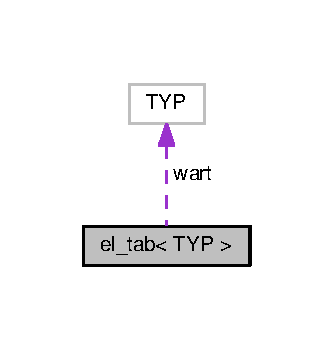
\includegraphics[width=160pt]{classel__tab__coll__graph}
\end{center}
\end{figure}
\subsection*{Metody publiczne}
\begin{DoxyCompactItemize}
\item 
\hyperlink{classel__tab_a62c9bef278f50d1e5f41b3fd3773b61d}{el\-\_\-tab} ()
\item 
\hyperlink{classel__tab_acb9e9041b31f9b2cf8224b6b8cebd935}{$\sim$el\-\_\-tab} ()
\end{DoxyCompactItemize}
\subsection*{Atrybuty publiczne}
\begin{DoxyCompactItemize}
\item 
string \hyperlink{classel__tab_a9a6e58703774b82293505e31aeac0e67}{klucz}
\begin{DoxyCompactList}\small\item\em identyfikator \end{DoxyCompactList}\item 
T\-Y\-P \hyperlink{classel__tab_a633bdedae8a85f29e0c27fa54c387dca}{wart}
\begin{DoxyCompactList}\small\item\em wartosc pola \end{DoxyCompactList}\item 
bool \hyperlink{classel__tab_aa757d12b4a8d169c50bd8e6b8d0d1fd2}{zajety}
\begin{DoxyCompactList}\small\item\em flaga informujaca, czy pole jest zajete \end{DoxyCompactList}\end{DoxyCompactItemize}


\subsection{Opis szczegółowy}
\subsubsection*{template$<$typename T\-Y\-P$>$class el\-\_\-tab$<$ T\-Y\-P $>$}

pojedynczy element tablicy haszujacej 

Definicja w linii 11 pliku hashtab.\-hh.



\subsection{Dokumentacja konstruktora i destruktora}
\hypertarget{classel__tab_a62c9bef278f50d1e5f41b3fd3773b61d}{\index{el\-\_\-tab@{el\-\_\-tab}!el\-\_\-tab@{el\-\_\-tab}}
\index{el\-\_\-tab@{el\-\_\-tab}!el_tab@{el\-\_\-tab}}
\subsubsection[{el\-\_\-tab}]{\setlength{\rightskip}{0pt plus 5cm}template$<$typename T\-Y\-P $>$ {\bf el\-\_\-tab}$<$ T\-Y\-P $>$\-::{\bf el\-\_\-tab} (
\begin{DoxyParamCaption}
{}
\end{DoxyParamCaption}
)\hspace{0.3cm}{\ttfamily [inline]}}}\label{classel__tab_a62c9bef278f50d1e5f41b3fd3773b61d}


Definicja w linii 26 pliku hashtab.\-hh.

\hypertarget{classel__tab_acb9e9041b31f9b2cf8224b6b8cebd935}{\index{el\-\_\-tab@{el\-\_\-tab}!$\sim$el\-\_\-tab@{$\sim$el\-\_\-tab}}
\index{$\sim$el\-\_\-tab@{$\sim$el\-\_\-tab}!el_tab@{el\-\_\-tab}}
\subsubsection[{$\sim$el\-\_\-tab}]{\setlength{\rightskip}{0pt plus 5cm}template$<$typename T\-Y\-P $>$ {\bf el\-\_\-tab}$<$ T\-Y\-P $>$\-::$\sim${\bf el\-\_\-tab} (
\begin{DoxyParamCaption}
{}
\end{DoxyParamCaption}
)\hspace{0.3cm}{\ttfamily [inline]}}}\label{classel__tab_acb9e9041b31f9b2cf8224b6b8cebd935}


Definicja w linii 27 pliku hashtab.\-hh.



\subsection{Dokumentacja atrybutów składowych}
\hypertarget{classel__tab_a9a6e58703774b82293505e31aeac0e67}{\index{el\-\_\-tab@{el\-\_\-tab}!klucz@{klucz}}
\index{klucz@{klucz}!el_tab@{el\-\_\-tab}}
\subsubsection[{klucz}]{\setlength{\rightskip}{0pt plus 5cm}template$<$typename T\-Y\-P $>$ string {\bf el\-\_\-tab}$<$ T\-Y\-P $>$\-::klucz}}\label{classel__tab_a9a6e58703774b82293505e31aeac0e67}


identyfikator 



Definicja w linii 16 pliku hashtab.\-hh.

\hypertarget{classel__tab_a633bdedae8a85f29e0c27fa54c387dca}{\index{el\-\_\-tab@{el\-\_\-tab}!wart@{wart}}
\index{wart@{wart}!el_tab@{el\-\_\-tab}}
\subsubsection[{wart}]{\setlength{\rightskip}{0pt plus 5cm}template$<$typename T\-Y\-P $>$ T\-Y\-P {\bf el\-\_\-tab}$<$ T\-Y\-P $>$\-::wart}}\label{classel__tab_a633bdedae8a85f29e0c27fa54c387dca}


wartosc pola 



Definicja w linii 21 pliku hashtab.\-hh.

\hypertarget{classel__tab_aa757d12b4a8d169c50bd8e6b8d0d1fd2}{\index{el\-\_\-tab@{el\-\_\-tab}!zajety@{zajety}}
\index{zajety@{zajety}!el_tab@{el\-\_\-tab}}
\subsubsection[{zajety}]{\setlength{\rightskip}{0pt plus 5cm}template$<$typename T\-Y\-P $>$ bool {\bf el\-\_\-tab}$<$ T\-Y\-P $>$\-::zajety}}\label{classel__tab_aa757d12b4a8d169c50bd8e6b8d0d1fd2}


flaga informujaca, czy pole jest zajete 



Definicja w linii 25 pliku hashtab.\-hh.



Dokumentacja dla tej klasy została wygenerowana z pliku\-:\begin{DoxyCompactItemize}
\item 
\hyperlink{hashtab_8hh}{hashtab.\-hh}\end{DoxyCompactItemize}

\hypertarget{classh__sort}{\section{\-Dokumentacja klasy h\-\_\-sort}
\label{classh__sort}\index{h\-\_\-sort@{h\-\_\-sort}}
}


klasa reprezentuje dane poddane sortowaniu przez kopcowanie  




{\ttfamily \#include $<$algorytm.\-hh$>$}



\-Diagram dziedziczenia dla h\-\_\-sort\nopagebreak
\begin{figure}[H]
\begin{center}
\leavevmode
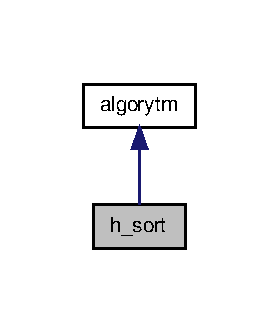
\includegraphics[width=134pt]{classh__sort__inherit__graph}
\end{center}
\end{figure}


\-Diagram współpracy dla h\-\_\-sort\-:\nopagebreak
\begin{figure}[H]
\begin{center}
\leavevmode
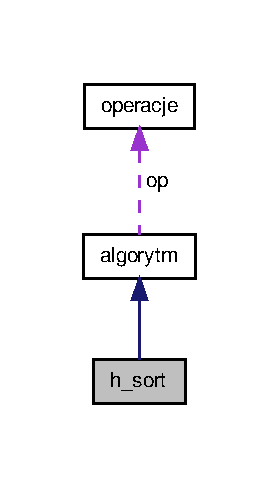
\includegraphics[width=134pt]{classh__sort__coll__graph}
\end{center}
\end{figure}
\subsection*{\-Metody publiczne}
\begin{DoxyCompactItemize}
\item 
\hyperlink{classh__sort_a27a9e6a24497264c3b9e0101f417e4ad}{h\-\_\-sort} (ifstream \&plik1, ifstream \&plik2, int \-N, int \-M)
\begin{DoxyCompactList}\small\item\em konstruktor klasy \end{DoxyCompactList}\item 
float \hyperlink{classh__sort_a496c249e58b48ca10e06266d1f673bd7}{przelicz} ()
\begin{DoxyCompactList}\small\item\em metoda dokonujaca sortowania danych \end{DoxyCompactList}\end{DoxyCompactItemize}


\subsection{\-Opis szczegółowy}
klasa reprezentuje dane poddane sortowaniu przez kopcowanie 

\-Definicja w linii 207 pliku algorytm.\-hh.



\subsection{\-Dokumentacja konstruktora i destruktora}
\hypertarget{classh__sort_a27a9e6a24497264c3b9e0101f417e4ad}{\index{h\-\_\-sort@{h\-\_\-sort}!h\-\_\-sort@{h\-\_\-sort}}
\index{h\-\_\-sort@{h\-\_\-sort}!h_sort@{h\-\_\-sort}}
\subsubsection[{h\-\_\-sort}]{\setlength{\rightskip}{0pt plus 5cm}{\bf h\-\_\-sort\-::h\-\_\-sort} (
\begin{DoxyParamCaption}
\item[{ifstream \&}]{plik1, }
\item[{ifstream \&}]{plik2, }
\item[{int}]{\-N, }
\item[{int}]{\-M}
\end{DoxyParamCaption}
)\hspace{0.3cm}{\ttfamily  \mbox{[}inline\mbox{]}}}}\label{classh__sort_a27a9e6a24497264c3b9e0101f417e4ad}


konstruktor klasy 



\-Definicja w linii 210 pliku algorytm.\-hh.



\subsection{\-Dokumentacja funkcji składowych}
\hypertarget{classh__sort_a496c249e58b48ca10e06266d1f673bd7}{\index{h\-\_\-sort@{h\-\_\-sort}!przelicz@{przelicz}}
\index{przelicz@{przelicz}!h_sort@{h\-\_\-sort}}
\subsubsection[{przelicz}]{\setlength{\rightskip}{0pt plus 5cm}float {\bf h\-\_\-sort\-::przelicz} (
\begin{DoxyParamCaption}
{}
\end{DoxyParamCaption}
)\hspace{0.3cm}{\ttfamily  \mbox{[}virtual\mbox{]}}}}\label{classh__sort_a496c249e58b48ca10e06266d1f673bd7}


metoda dokonujaca sortowania danych 



\-Reimplementowana z \hyperlink{classalgorytm_af3f92bf537b1f2e1f93173983e838449}{algorytm}.



\-Definicja w linii 180 pliku algorytm.\-cpp.



\-Oto graf wywołań dla tej funkcji\-:\nopagebreak
\begin{figure}[H]
\begin{center}
\leavevmode
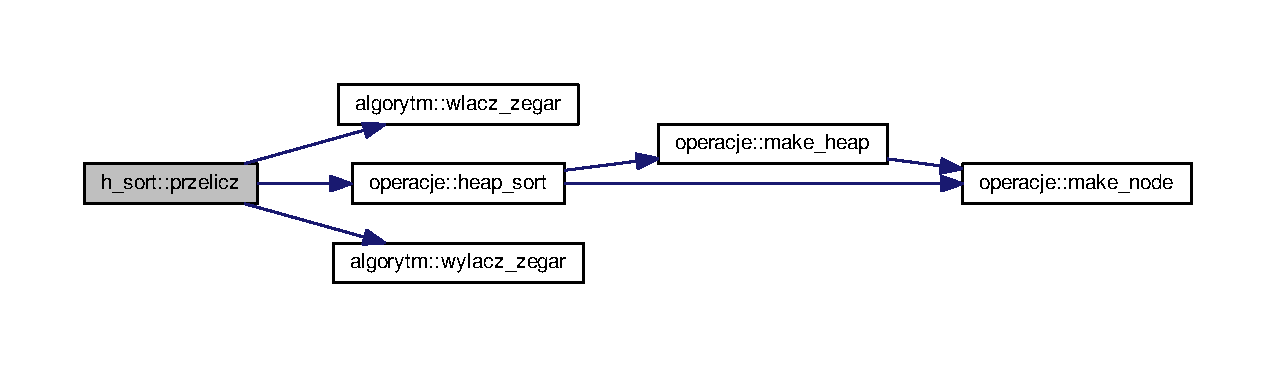
\includegraphics[width=350pt]{classh__sort_a496c249e58b48ca10e06266d1f673bd7_cgraph}
\end{center}
\end{figure}




\-Dokumentacja dla tej klasy została wygenerowana z plików\-:\begin{DoxyCompactItemize}
\item 
\hyperlink{algorytm_8hh}{algorytm.\-hh}\item 
\hyperlink{algorytm_8cpp}{algorytm.\-cpp}\end{DoxyCompactItemize}

\hypertarget{classh__table}{\section{\-Dokumentacja klasy h\-\_\-table}
\label{classh__table}\index{h\-\_\-table@{h\-\_\-table}}
}


\-Modeluje tablice haszujaca przeznaczona do testowania szybkosci wyszukiwnaia.  




{\ttfamily \#include $<$algorytm.\-hh$>$}



\-Diagram dziedziczenia dla h\-\_\-table\nopagebreak
\begin{figure}[H]
\begin{center}
\leavevmode
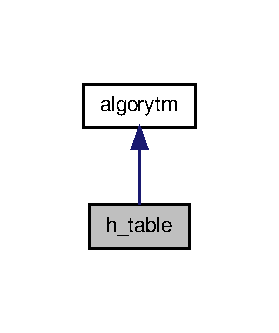
\includegraphics[width=134pt]{classh__table__inherit__graph}
\end{center}
\end{figure}


\-Diagram współpracy dla h\-\_\-table\-:\nopagebreak
\begin{figure}[H]
\begin{center}
\leavevmode
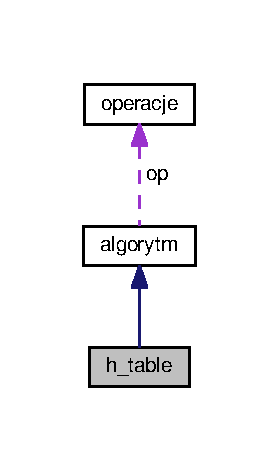
\includegraphics[width=134pt]{classh__table__coll__graph}
\end{center}
\end{figure}
\subsection*{\-Metody publiczne}
\begin{DoxyCompactItemize}
\item 
void \hyperlink{classh__table_a938885a9ce57ae0c447dd9a146637ce9}{wczytaj\-\_\-klucze} (ifstream \&plik)
\begin{DoxyCompactList}\small\item\em wczytywanie kluczy \end{DoxyCompactList}\item 
\hyperlink{classh__table_add097e1c13f110997c50b57f7d5e4cf5}{h\-\_\-table} (ifstream \&plik1, ifstream \&plik2, ifstream \&plik3, int \-N, int \-M)
\begin{DoxyCompactList}\small\item\em konstruktor \end{DoxyCompactList}\item 
float \hyperlink{classh__table_a8726955778aed30773dccf8e0cb81064}{przelicz} ()
\begin{DoxyCompactList}\small\item\em \-Metoda odpowiada za przetworzenie danych wejsciowych zgodnie z zadanym algorytmem. \end{DoxyCompactList}\end{DoxyCompactItemize}
\subsection*{\-Atrybuty prywatne}
\begin{DoxyCompactItemize}
\item 
string $\ast$ \hyperlink{classh__table_af7ef9b7c0043f4320e5b8fd9ce3678d5}{klucze}
\begin{DoxyCompactList}\small\item\em tablica kluczy \end{DoxyCompactList}\end{DoxyCompactItemize}


\subsection{\-Opis szczegółowy}
\-Modeluje tablice haszujaca przeznaczona do testowania szybkosci wyszukiwnaia. 

\-Definicja w linii 246 pliku algorytm.\-hh.



\subsection{\-Dokumentacja konstruktora i destruktora}
\hypertarget{classh__table_add097e1c13f110997c50b57f7d5e4cf5}{\index{h\-\_\-table@{h\-\_\-table}!h\-\_\-table@{h\-\_\-table}}
\index{h\-\_\-table@{h\-\_\-table}!h_table@{h\-\_\-table}}
\subsubsection[{h\-\_\-table}]{\setlength{\rightskip}{0pt plus 5cm}{\bf h\-\_\-table\-::h\-\_\-table} (
\begin{DoxyParamCaption}
\item[{ifstream \&}]{plik1, }
\item[{ifstream \&}]{plik2, }
\item[{ifstream \&}]{plik3, }
\item[{int}]{\-N, }
\item[{int}]{\-M}
\end{DoxyParamCaption}
)\hspace{0.3cm}{\ttfamily  \mbox{[}inline\mbox{]}}}}\label{classh__table_add097e1c13f110997c50b57f7d5e4cf5}


konstruktor 



\-Definicja w linii 255 pliku algorytm.\-hh.



\subsection{\-Dokumentacja funkcji składowych}
\hypertarget{classh__table_a8726955778aed30773dccf8e0cb81064}{\index{h\-\_\-table@{h\-\_\-table}!przelicz@{przelicz}}
\index{przelicz@{przelicz}!h_table@{h\-\_\-table}}
\subsubsection[{przelicz}]{\setlength{\rightskip}{0pt plus 5cm}float {\bf h\-\_\-table\-::przelicz} (
\begin{DoxyParamCaption}
{}
\end{DoxyParamCaption}
)\hspace{0.3cm}{\ttfamily  \mbox{[}virtual\mbox{]}}}}\label{classh__table_a8726955778aed30773dccf8e0cb81064}


\-Metoda odpowiada za przetworzenie danych wejsciowych zgodnie z zadanym algorytmem. 



\-Reimplementowana z \hyperlink{classalgorytm_af3f92bf537b1f2e1f93173983e838449}{algorytm}.



\-Definicja w linii 219 pliku algorytm.\-cpp.



\-Oto graf wywołań dla tej funkcji\-:\nopagebreak
\begin{figure}[H]
\begin{center}
\leavevmode
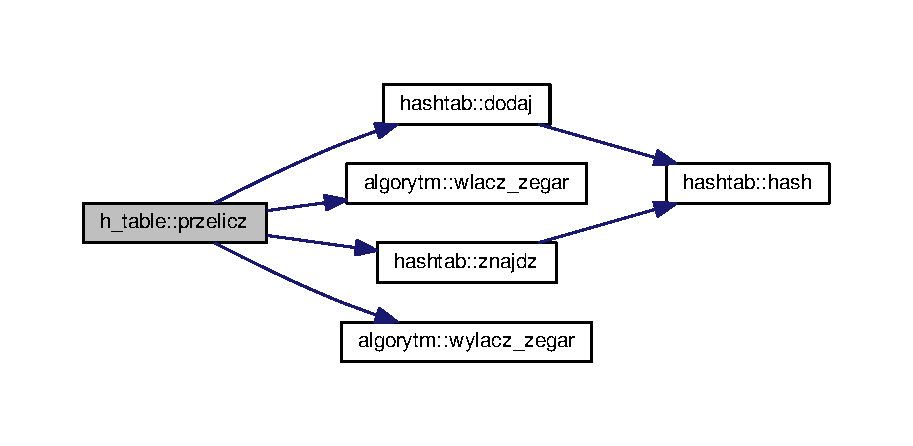
\includegraphics[width=350pt]{classh__table_a8726955778aed30773dccf8e0cb81064_cgraph}
\end{center}
\end{figure}


\hypertarget{classh__table_a938885a9ce57ae0c447dd9a146637ce9}{\index{h\-\_\-table@{h\-\_\-table}!wczytaj\-\_\-klucze@{wczytaj\-\_\-klucze}}
\index{wczytaj\-\_\-klucze@{wczytaj\-\_\-klucze}!h_table@{h\-\_\-table}}
\subsubsection[{wczytaj\-\_\-klucze}]{\setlength{\rightskip}{0pt plus 5cm}void {\bf h\-\_\-table\-::wczytaj\-\_\-klucze} (
\begin{DoxyParamCaption}
\item[{ifstream \&}]{plik}
\end{DoxyParamCaption}
)}}\label{classh__table_a938885a9ce57ae0c447dd9a146637ce9}


wczytywanie kluczy 


\begin{DoxyParams}[1]{\-Parametry}
\mbox{\tt in}  & {\em plik} & -\/ strumien z kluczmai uzytymi podczas testow \\
\hline
\end{DoxyParams}


\-Definicja w linii 213 pliku algorytm.\-cpp.



\subsection{\-Dokumentacja atrybutów składowych}
\hypertarget{classh__table_af7ef9b7c0043f4320e5b8fd9ce3678d5}{\index{h\-\_\-table@{h\-\_\-table}!klucze@{klucze}}
\index{klucze@{klucze}!h_table@{h\-\_\-table}}
\subsubsection[{klucze}]{\setlength{\rightskip}{0pt plus 5cm}string$\ast$ {\bf h\-\_\-table\-::klucze}\hspace{0.3cm}{\ttfamily  \mbox{[}private\mbox{]}}}}\label{classh__table_af7ef9b7c0043f4320e5b8fd9ce3678d5}


tablica kluczy 



\-Definicja w linii 248 pliku algorytm.\-hh.



\-Dokumentacja dla tej klasy została wygenerowana z plików\-:\begin{DoxyCompactItemize}
\item 
\hyperlink{algorytm_8hh}{algorytm.\-hh}\item 
\hyperlink{algorytm_8cpp}{algorytm.\-cpp}\end{DoxyCompactItemize}

\hypertarget{classhashtab}{\section{\-Dokumentacja szablonu klasy hashtab$<$ \-T\-Y\-P $>$}
\label{classhashtab}\index{hashtab$<$ T\-Y\-P $>$@{hashtab$<$ T\-Y\-P $>$}}
}


modeluje tablice haszujca w oparciu o kontener klasy \hyperlink{classel__tab}{el\-\_\-tab}  




{\ttfamily \#include $<$hashtab.\-hh$>$}

\subsection*{\-Metody publiczne}
\begin{DoxyCompactItemize}
\item 
void \hyperlink{classhashtab_a94671e2fe307f5248c0b1b6855d4c3d4}{ustaw\-\_\-dlugosc} (int d)
\begin{DoxyCompactList}\small\item\em ustawia dlugosc tablicy \end{DoxyCompactList}\item 
\hyperlink{classhashtab_abcac01cb8d855d39b9d766a6f16856ee}{hashtab} ()
\begin{DoxyCompactList}\small\item\em konstruktor bezparametryczny \end{DoxyCompactList}\item 
\hyperlink{classhashtab_aa7315b45b8b2251113cc6d9c8d606bb8}{hashtab} (int \-N)
\begin{DoxyCompactList}\small\item\em konsruktor parametryczny \end{DoxyCompactList}\item 
unsigned long \hyperlink{classhashtab_ad52a5a127bcfe2b93bbec7fe702f10a6}{hash} (string k)
\begin{DoxyCompactList}\small\item\em funkcja haszujaca \end{DoxyCompactList}\item 
void \hyperlink{classhashtab_ad25515f0b7a631904c65b57f834c428f}{dodaj} (string k, \-T\-Y\-P v)
\begin{DoxyCompactList}\small\item\em metoda dodaje element do tablicy hasuzjacej \end{DoxyCompactList}\item 
\hyperlink{classel__tab}{el\-\_\-tab}$<$ \-T\-Y\-P $>$ $\ast$ \hyperlink{classhashtab_af6452a7dbb4a30870ec16635b859f18c}{znajdz} (string k)
\begin{DoxyCompactList}\small\item\em metoda szuka zadanego elementu w oparciu o klucz \end{DoxyCompactList}\item 
void \hyperlink{classhashtab_a2c0b494972d78d893a6db6c08b8af3a2}{usun} (string k)
\begin{DoxyCompactList}\small\item\em usuwa element jesli znajduje sie w tablicy \end{DoxyCompactList}\item 
void \hyperlink{classhashtab_a69b5dcc5943caf7afb74a98f461a1c1b}{wypisz} ()
\end{DoxyCompactItemize}
\subsection*{\-Atrybuty prywatne}
\begin{DoxyCompactItemize}
\item 
int \hyperlink{classhashtab_a1c0fe6f05d425274c58352e21cc7f496}{dlugosc}
\begin{DoxyCompactList}\small\item\em dlugosc tablicy \end{DoxyCompactList}\item 
vector$<$ \hyperlink{classel__tab}{el\-\_\-tab}$<$ \-T\-Y\-P $>$ $>$ \hyperlink{classhashtab_ab7d4d7c920e89fae8a292772dc9d7611}{tab}
\begin{DoxyCompactList}\small\item\em tablica haszujaca \end{DoxyCompactList}\end{DoxyCompactItemize}


\subsection{\-Opis szczegółowy}
\subsubsection*{template$<$typename \-T\-Y\-P$>$class hashtab$<$ T\-Y\-P $>$}

modeluje tablice haszujca w oparciu o kontener klasy \hyperlink{classel__tab}{el\-\_\-tab} 

\-Definicja w linii 34 pliku hashtab.\-hh.



\subsection{\-Dokumentacja konstruktora i destruktora}
\hypertarget{classhashtab_abcac01cb8d855d39b9d766a6f16856ee}{\index{hashtab@{hashtab}!hashtab@{hashtab}}
\index{hashtab@{hashtab}!hashtab@{hashtab}}
\subsubsection[{hashtab}]{\setlength{\rightskip}{0pt plus 5cm}template$<$typename \-T\-Y\-P$>$ {\bf hashtab}$<$ \-T\-Y\-P $>$\-::{\bf hashtab} (
\begin{DoxyParamCaption}
{}
\end{DoxyParamCaption}
)\hspace{0.3cm}{\ttfamily  \mbox{[}inline\mbox{]}}}}\label{classhashtab_abcac01cb8d855d39b9d766a6f16856ee}


konstruktor bezparametryczny 



\-Definicja w linii 43 pliku hashtab.\-hh.

\hypertarget{classhashtab_aa7315b45b8b2251113cc6d9c8d606bb8}{\index{hashtab@{hashtab}!hashtab@{hashtab}}
\index{hashtab@{hashtab}!hashtab@{hashtab}}
\subsubsection[{hashtab}]{\setlength{\rightskip}{0pt plus 5cm}template$<$typename \-T\-Y\-P$>$ {\bf hashtab}$<$ \-T\-Y\-P $>$\-::{\bf hashtab} (
\begin{DoxyParamCaption}
\item[{int}]{\-N}
\end{DoxyParamCaption}
)\hspace{0.3cm}{\ttfamily  \mbox{[}inline\mbox{]}}}}\label{classhashtab_aa7315b45b8b2251113cc6d9c8d606bb8}


konsruktor parametryczny 


\begin{DoxyParams}[1]{\-Parametry}
\mbox{\tt in}  & {\em \-N} & -\/ rozmiar tablicy \\
\hline
\end{DoxyParams}


\-Definicja w linii 47 pliku hashtab.\-hh.



\-Oto graf wywołań dla tej funkcji\-:\nopagebreak
\begin{figure}[H]
\begin{center}
\leavevmode
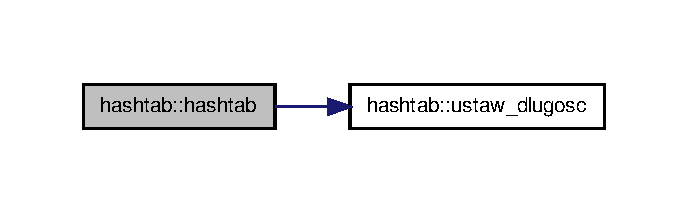
\includegraphics[width=330pt]{classhashtab_aa7315b45b8b2251113cc6d9c8d606bb8_cgraph}
\end{center}
\end{figure}




\subsection{\-Dokumentacja funkcji składowych}
\hypertarget{classhashtab_ad25515f0b7a631904c65b57f834c428f}{\index{hashtab@{hashtab}!dodaj@{dodaj}}
\index{dodaj@{dodaj}!hashtab@{hashtab}}
\subsubsection[{dodaj}]{\setlength{\rightskip}{0pt plus 5cm}template$<$typename \-T\-Y\-P$>$ void {\bf hashtab}$<$ \-T\-Y\-P $>$\-::{\bf dodaj} (
\begin{DoxyParamCaption}
\item[{string}]{k, }
\item[{\-T\-Y\-P}]{v}
\end{DoxyParamCaption}
)\hspace{0.3cm}{\ttfamily  \mbox{[}inline\mbox{]}}}}\label{classhashtab_ad25515f0b7a631904c65b57f834c428f}


metoda dodaje element do tablicy hasuzjacej 



\-Definicja w linii 59 pliku hashtab.\-hh.



\-Oto graf wywołań dla tej funkcji\-:\nopagebreak
\begin{figure}[H]
\begin{center}
\leavevmode
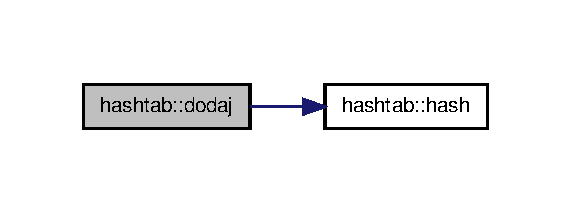
\includegraphics[width=274pt]{classhashtab_ad25515f0b7a631904c65b57f834c428f_cgraph}
\end{center}
\end{figure}




\-Oto graf wywoływań tej funkcji\-:\nopagebreak
\begin{figure}[H]
\begin{center}
\leavevmode
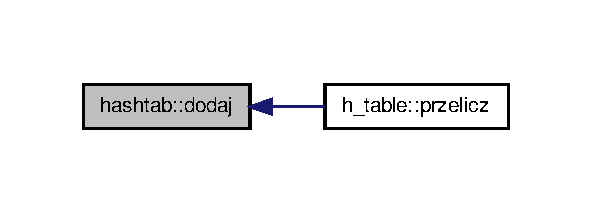
\includegraphics[width=284pt]{classhashtab_ad25515f0b7a631904c65b57f834c428f_icgraph}
\end{center}
\end{figure}


\hypertarget{classhashtab_ad52a5a127bcfe2b93bbec7fe702f10a6}{\index{hashtab@{hashtab}!hash@{hash}}
\index{hash@{hash}!hashtab@{hashtab}}
\subsubsection[{hash}]{\setlength{\rightskip}{0pt plus 5cm}template$<$typename \-T\-Y\-P$>$ unsigned long {\bf hashtab}$<$ \-T\-Y\-P $>$\-::{\bf hash} (
\begin{DoxyParamCaption}
\item[{string}]{k}
\end{DoxyParamCaption}
)\hspace{0.3cm}{\ttfamily  \mbox{[}inline\mbox{]}}}}\label{classhashtab_ad52a5a127bcfe2b93bbec7fe702f10a6}


funkcja haszujaca 

\begin{DoxyReturn}{\-Zwraca}
h -\/ liczba, ktora po kompresji bedzie indeksem danego elementu 
\end{DoxyReturn}


\-Definicja w linii 51 pliku hashtab.\-hh.



\-Oto graf wywoływań tej funkcji\-:\nopagebreak
\begin{figure}[H]
\begin{center}
\leavevmode
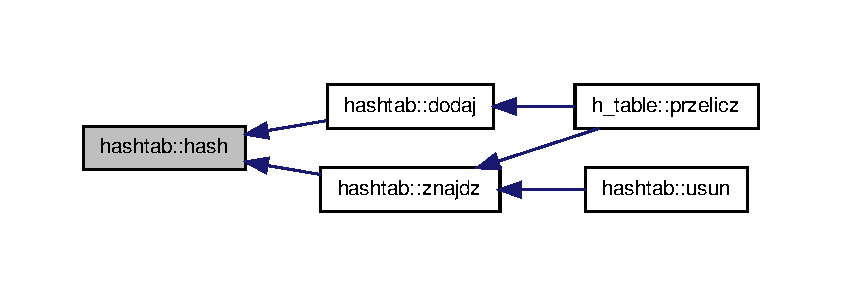
\includegraphics[width=350pt]{classhashtab_ad52a5a127bcfe2b93bbec7fe702f10a6_icgraph}
\end{center}
\end{figure}


\hypertarget{classhashtab_a94671e2fe307f5248c0b1b6855d4c3d4}{\index{hashtab@{hashtab}!ustaw\-\_\-dlugosc@{ustaw\-\_\-dlugosc}}
\index{ustaw\-\_\-dlugosc@{ustaw\-\_\-dlugosc}!hashtab@{hashtab}}
\subsubsection[{ustaw\-\_\-dlugosc}]{\setlength{\rightskip}{0pt plus 5cm}template$<$typename \-T\-Y\-P$>$ void {\bf hashtab}$<$ \-T\-Y\-P $>$\-::{\bf ustaw\-\_\-dlugosc} (
\begin{DoxyParamCaption}
\item[{int}]{d}
\end{DoxyParamCaption}
)\hspace{0.3cm}{\ttfamily  \mbox{[}inline\mbox{]}}}}\label{classhashtab_a94671e2fe307f5248c0b1b6855d4c3d4}


ustawia dlugosc tablicy 



\-Definicja w linii 41 pliku hashtab.\-hh.



\-Oto graf wywoływań tej funkcji\-:\nopagebreak
\begin{figure}[H]
\begin{center}
\leavevmode
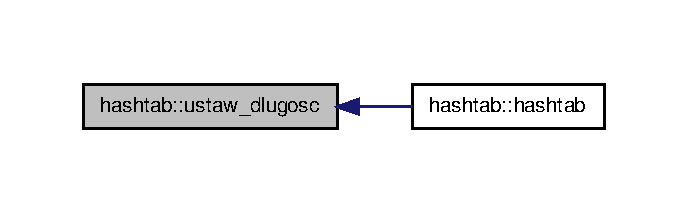
\includegraphics[width=330pt]{classhashtab_a94671e2fe307f5248c0b1b6855d4c3d4_icgraph}
\end{center}
\end{figure}


\hypertarget{classhashtab_a2c0b494972d78d893a6db6c08b8af3a2}{\index{hashtab@{hashtab}!usun@{usun}}
\index{usun@{usun}!hashtab@{hashtab}}
\subsubsection[{usun}]{\setlength{\rightskip}{0pt plus 5cm}template$<$typename \-T\-Y\-P$>$ void {\bf hashtab}$<$ \-T\-Y\-P $>$\-::{\bf usun} (
\begin{DoxyParamCaption}
\item[{string}]{k}
\end{DoxyParamCaption}
)\hspace{0.3cm}{\ttfamily  \mbox{[}inline\mbox{]}}}}\label{classhashtab_a2c0b494972d78d893a6db6c08b8af3a2}


usuwa element jesli znajduje sie w tablicy 


\begin{DoxyParams}[1]{\-Parametry}
\mbox{\tt in}  & {\em k} & -\/ klucz \\
\hline
\end{DoxyParams}


\-Definicja w linii 89 pliku hashtab.\-hh.



\-Oto graf wywołań dla tej funkcji\-:\nopagebreak
\begin{figure}[H]
\begin{center}
\leavevmode
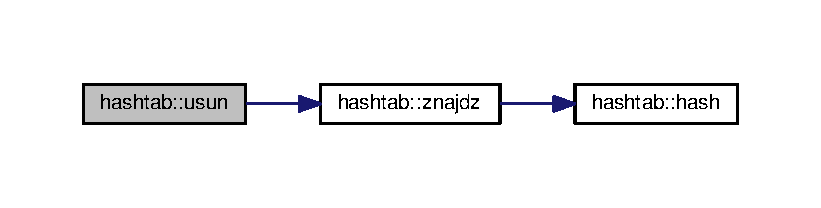
\includegraphics[width=350pt]{classhashtab_a2c0b494972d78d893a6db6c08b8af3a2_cgraph}
\end{center}
\end{figure}


\hypertarget{classhashtab_a69b5dcc5943caf7afb74a98f461a1c1b}{\index{hashtab@{hashtab}!wypisz@{wypisz}}
\index{wypisz@{wypisz}!hashtab@{hashtab}}
\subsubsection[{wypisz}]{\setlength{\rightskip}{0pt plus 5cm}template$<$typename \-T\-Y\-P$>$ void {\bf hashtab}$<$ \-T\-Y\-P $>$\-::{\bf wypisz} (
\begin{DoxyParamCaption}
{}
\end{DoxyParamCaption}
)\hspace{0.3cm}{\ttfamily  \mbox{[}inline\mbox{]}}}}\label{classhashtab_a69b5dcc5943caf7afb74a98f461a1c1b}


\-Definicja w linii 93 pliku hashtab.\-hh.

\hypertarget{classhashtab_af6452a7dbb4a30870ec16635b859f18c}{\index{hashtab@{hashtab}!znajdz@{znajdz}}
\index{znajdz@{znajdz}!hashtab@{hashtab}}
\subsubsection[{znajdz}]{\setlength{\rightskip}{0pt plus 5cm}template$<$typename \-T\-Y\-P$>$ {\bf el\-\_\-tab}$<$\-T\-Y\-P$>$$\ast$ {\bf hashtab}$<$ \-T\-Y\-P $>$\-::{\bf znajdz} (
\begin{DoxyParamCaption}
\item[{string}]{k}
\end{DoxyParamCaption}
)\hspace{0.3cm}{\ttfamily  \mbox{[}inline\mbox{]}}}}\label{classhashtab_af6452a7dbb4a30870ec16635b859f18c}


metoda szuka zadanego elementu w oparciu o klucz 


\begin{DoxyParams}[1]{\-Parametry}
\mbox{\tt in}  & {\em k} & -\/ klucz elementu \\
\hline
\end{DoxyParams}
\begin{DoxyReturn}{\-Zwraca}
znaleziony element 
\end{DoxyReturn}


\-Definicja w linii 74 pliku hashtab.\-hh.



\-Oto graf wywołań dla tej funkcji\-:\nopagebreak
\begin{figure}[H]
\begin{center}
\leavevmode
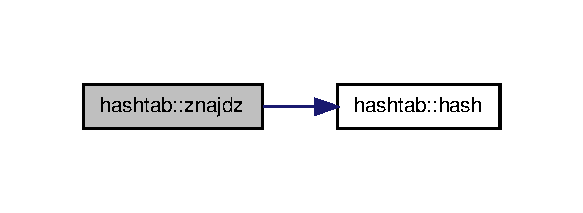
\includegraphics[width=280pt]{classhashtab_af6452a7dbb4a30870ec16635b859f18c_cgraph}
\end{center}
\end{figure}




\-Oto graf wywoływań tej funkcji\-:\nopagebreak
\begin{figure}[H]
\begin{center}
\leavevmode
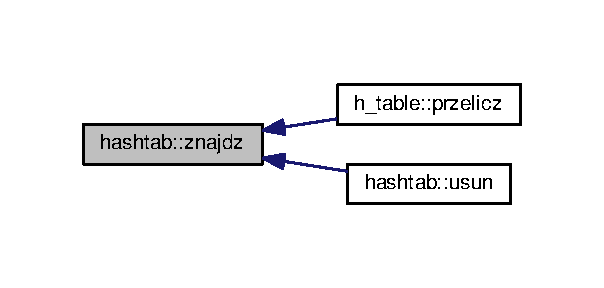
\includegraphics[width=290pt]{classhashtab_af6452a7dbb4a30870ec16635b859f18c_icgraph}
\end{center}
\end{figure}




\subsection{\-Dokumentacja atrybutów składowych}
\hypertarget{classhashtab_a1c0fe6f05d425274c58352e21cc7f496}{\index{hashtab@{hashtab}!dlugosc@{dlugosc}}
\index{dlugosc@{dlugosc}!hashtab@{hashtab}}
\subsubsection[{dlugosc}]{\setlength{\rightskip}{0pt plus 5cm}template$<$typename \-T\-Y\-P$>$ int {\bf hashtab}$<$ \-T\-Y\-P $>$\-::{\bf dlugosc}\hspace{0.3cm}{\ttfamily  \mbox{[}private\mbox{]}}}}\label{classhashtab_a1c0fe6f05d425274c58352e21cc7f496}


dlugosc tablicy 



\-Definicja w linii 36 pliku hashtab.\-hh.

\hypertarget{classhashtab_ab7d4d7c920e89fae8a292772dc9d7611}{\index{hashtab@{hashtab}!tab@{tab}}
\index{tab@{tab}!hashtab@{hashtab}}
\subsubsection[{tab}]{\setlength{\rightskip}{0pt plus 5cm}template$<$typename \-T\-Y\-P$>$ vector$<${\bf el\-\_\-tab}$<$\-T\-Y\-P$>$ $>$ {\bf hashtab}$<$ \-T\-Y\-P $>$\-::{\bf tab}\hspace{0.3cm}{\ttfamily  \mbox{[}private\mbox{]}}}}\label{classhashtab_ab7d4d7c920e89fae8a292772dc9d7611}


tablica haszujaca 



\-Definicja w linii 38 pliku hashtab.\-hh.



\-Dokumentacja dla tej klasy została wygenerowana z pliku\-:\begin{DoxyCompactItemize}
\item 
\hyperlink{hashtab_8hh}{hashtab.\-hh}\end{DoxyCompactItemize}

\hypertarget{classkolejka__lista}{\section{\-Dokumentacja klasy kolejka\-\_\-lista}
\label{classkolejka__lista}\index{kolejka\-\_\-lista@{kolejka\-\_\-lista}}
}


klasa utworzona na potrzeby pomiaru czasu wypełnienia struktury  




{\ttfamily \#include $<$algorytm.\-hh$>$}



\-Diagram dziedziczenia dla kolejka\-\_\-lista\nopagebreak
\begin{figure}[H]
\begin{center}
\leavevmode
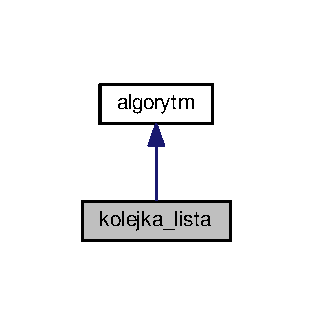
\includegraphics[width=150pt]{classkolejka__lista__inherit__graph}
\end{center}
\end{figure}


\-Diagram współpracy dla kolejka\-\_\-lista\-:\nopagebreak
\begin{figure}[H]
\begin{center}
\leavevmode
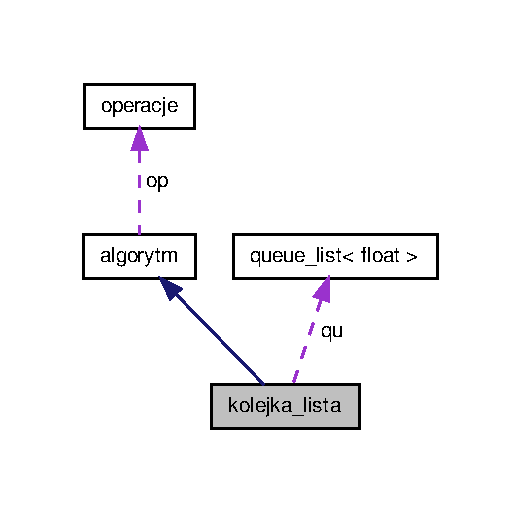
\includegraphics[width=250pt]{classkolejka__lista__coll__graph}
\end{center}
\end{figure}
\subsection*{\-Metody publiczne}
\begin{DoxyCompactItemize}
\item 
\hyperlink{classkolejka__lista_a5472805c319e05803d4841aecfd0c910}{kolejka\-\_\-lista} (ifstream \&plik1, ifstream \&plik2, int \-N, int \-M)
\item 
float \hyperlink{classkolejka__lista_a239ae8bcd2dcee9b79945010e0e32037}{przelicz} ()
\begin{DoxyCompactList}\small\item\em \-Metoda odpowiada za przetworzenie danych wejsciowych zgodnie z zadanym algorytmem. \end{DoxyCompactList}\end{DoxyCompactItemize}
\subsection*{\-Atrybuty prywatne}
\begin{DoxyCompactItemize}
\item 
\hyperlink{classqueue__list}{queue\-\_\-list}$<$ float $>$ \hyperlink{classkolejka__lista_a5e378458ccfc86d903b1a71a8ff5bad8}{qu}
\end{DoxyCompactItemize}


\subsection{\-Opis szczegółowy}
klasa utworzona na potrzeby pomiaru czasu wypełnienia struktury 

\-Definicja w linii 186 pliku algorytm.\-hh.



\subsection{\-Dokumentacja konstruktora i destruktora}
\hypertarget{classkolejka__lista_a5472805c319e05803d4841aecfd0c910}{\index{kolejka\-\_\-lista@{kolejka\-\_\-lista}!kolejka\-\_\-lista@{kolejka\-\_\-lista}}
\index{kolejka\-\_\-lista@{kolejka\-\_\-lista}!kolejka_lista@{kolejka\-\_\-lista}}
\subsubsection[{kolejka\-\_\-lista}]{\setlength{\rightskip}{0pt plus 5cm}{\bf kolejka\-\_\-lista\-::kolejka\-\_\-lista} (
\begin{DoxyParamCaption}
\item[{ifstream \&}]{plik1, }
\item[{ifstream \&}]{plik2, }
\item[{int}]{\-N, }
\item[{int}]{\-M}
\end{DoxyParamCaption}
)\hspace{0.3cm}{\ttfamily  \mbox{[}inline\mbox{]}}}}\label{classkolejka__lista_a5472805c319e05803d4841aecfd0c910}


\-Definicja w linii 189 pliku algorytm.\-hh.



\subsection{\-Dokumentacja funkcji składowych}
\hypertarget{classkolejka__lista_a239ae8bcd2dcee9b79945010e0e32037}{\index{kolejka\-\_\-lista@{kolejka\-\_\-lista}!przelicz@{przelicz}}
\index{przelicz@{przelicz}!kolejka_lista@{kolejka\-\_\-lista}}
\subsubsection[{przelicz}]{\setlength{\rightskip}{0pt plus 5cm}float {\bf kolejka\-\_\-lista\-::przelicz} (
\begin{DoxyParamCaption}
{}
\end{DoxyParamCaption}
)\hspace{0.3cm}{\ttfamily  \mbox{[}virtual\mbox{]}}}}\label{classkolejka__lista_a239ae8bcd2dcee9b79945010e0e32037}


\-Metoda odpowiada za przetworzenie danych wejsciowych zgodnie z zadanym algorytmem. 



\-Reimplementowana z \hyperlink{classalgorytm_af3f92bf537b1f2e1f93173983e838449}{algorytm}.



\-Definicja w linii 143 pliku algorytm.\-cpp.



\-Oto graf wywołań dla tej funkcji\-:\nopagebreak
\begin{figure}[H]
\begin{center}
\leavevmode
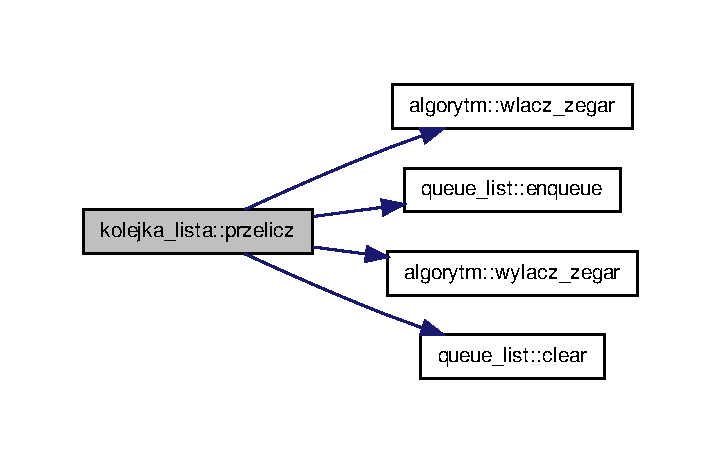
\includegraphics[width=346pt]{classkolejka__lista_a239ae8bcd2dcee9b79945010e0e32037_cgraph}
\end{center}
\end{figure}




\subsection{\-Dokumentacja atrybutów składowych}
\hypertarget{classkolejka__lista_a5e378458ccfc86d903b1a71a8ff5bad8}{\index{kolejka\-\_\-lista@{kolejka\-\_\-lista}!qu@{qu}}
\index{qu@{qu}!kolejka_lista@{kolejka\-\_\-lista}}
\subsubsection[{qu}]{\setlength{\rightskip}{0pt plus 5cm}{\bf queue\-\_\-list}$<$float$>$ {\bf kolejka\-\_\-lista\-::qu}\hspace{0.3cm}{\ttfamily  \mbox{[}private\mbox{]}}}}\label{classkolejka__lista_a5e378458ccfc86d903b1a71a8ff5bad8}


\-Definicja w linii 187 pliku algorytm.\-hh.



\-Dokumentacja dla tej klasy została wygenerowana z plików\-:\begin{DoxyCompactItemize}
\item 
\hyperlink{algorytm_8hh}{algorytm.\-hh}\item 
\hyperlink{algorytm_8cpp}{algorytm.\-cpp}\end{DoxyCompactItemize}

\hypertarget{classkolejka__tablica}{\section{Dokumentacja klasy kolejka\-\_\-tablica}
\label{classkolejka__tablica}\index{kolejka\-\_\-tablica@{kolejka\-\_\-tablica}}
}


klasa utworzona na potrzeby pomiaru czasu wypełnienia struktury  




{\ttfamily \#include $<$algorytm.\-hh$>$}



Diagram dziedziczenia dla kolejka\-\_\-tablica\nopagebreak
\begin{figure}[H]
\begin{center}
\leavevmode
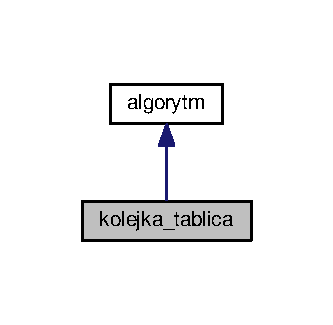
\includegraphics[width=160pt]{classkolejka__tablica__inherit__graph}
\end{center}
\end{figure}


Diagram współpracy dla kolejka\-\_\-tablica\-:\nopagebreak
\begin{figure}[H]
\begin{center}
\leavevmode
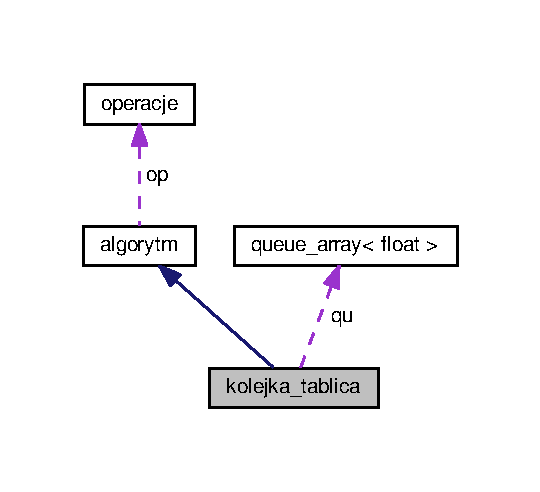
\includegraphics[width=259pt]{classkolejka__tablica__coll__graph}
\end{center}
\end{figure}
\subsection*{Metody publiczne}
\begin{DoxyCompactItemize}
\item 
\hyperlink{classkolejka__tablica_aa99b89749fcd8c780882ebbe089cad0f}{kolejka\-\_\-tablica} (ifstream \&plik1, ifstream \&plik2, int N, int M, \hyperlink{stos_8hh_a7847560c748814fd3070e9149a9578bd}{flag} F)
\begin{DoxyCompactList}\small\item\em konstruktor -\/ ustawia flage w zadany stan \end{DoxyCompactList}\item 
float \hyperlink{classkolejka__tablica_aad6baa28ce61111666e70df7d6ac4f86}{przelicz} ()
\begin{DoxyCompactList}\small\item\em Metoda odpowiada za przetworzenie danych wejsciowych zgodnie z zadanym algorytmem. \end{DoxyCompactList}\end{DoxyCompactItemize}
\subsection*{Atrybuty prywatne}
\begin{DoxyCompactItemize}
\item 
\hyperlink{classqueue__array}{queue\-\_\-array}$<$ float $>$ \hyperlink{classkolejka__tablica_a7fd15c7c7a0fa3649042ec634b2b8d4f}{qu}
\end{DoxyCompactItemize}
\subsection*{Dodatkowe Dziedziczone Składowe}


\subsection{Opis szczegółowy}
klasa utworzona na potrzeby pomiaru czasu wypełnienia struktury 

Definicja w linii 179 pliku algorytm.\-hh.



\subsection{Dokumentacja konstruktora i destruktora}
\hypertarget{classkolejka__tablica_aa99b89749fcd8c780882ebbe089cad0f}{\index{kolejka\-\_\-tablica@{kolejka\-\_\-tablica}!kolejka\-\_\-tablica@{kolejka\-\_\-tablica}}
\index{kolejka\-\_\-tablica@{kolejka\-\_\-tablica}!kolejka_tablica@{kolejka\-\_\-tablica}}
\subsubsection[{kolejka\-\_\-tablica}]{\setlength{\rightskip}{0pt plus 5cm}kolejka\-\_\-tablica\-::kolejka\-\_\-tablica (
\begin{DoxyParamCaption}
\item[{ifstream \&}]{plik1, }
\item[{ifstream \&}]{plik2, }
\item[{int}]{N, }
\item[{int}]{M, }
\item[{{\bf flag}}]{F}
\end{DoxyParamCaption}
)\hspace{0.3cm}{\ttfamily [inline]}}}\label{classkolejka__tablica_aa99b89749fcd8c780882ebbe089cad0f}


konstruktor -\/ ustawia flage w zadany stan 



Definicja w linii 185 pliku algorytm.\-hh.



\subsection{Dokumentacja funkcji składowych}
\hypertarget{classkolejka__tablica_aad6baa28ce61111666e70df7d6ac4f86}{\index{kolejka\-\_\-tablica@{kolejka\-\_\-tablica}!przelicz@{przelicz}}
\index{przelicz@{przelicz}!kolejka_tablica@{kolejka\-\_\-tablica}}
\subsubsection[{przelicz}]{\setlength{\rightskip}{0pt plus 5cm}float kolejka\-\_\-tablica\-::przelicz (
\begin{DoxyParamCaption}
{}
\end{DoxyParamCaption}
)\hspace{0.3cm}{\ttfamily [virtual]}}}\label{classkolejka__tablica_aad6baa28ce61111666e70df7d6ac4f86}


Metoda odpowiada za przetworzenie danych wejsciowych zgodnie z zadanym algorytmem. 



Reimplementowana z \hyperlink{classalgorytm_af3f92bf537b1f2e1f93173983e838449}{algorytm}.



Definicja w linii 148 pliku algorytm.\-cpp.



Oto graf wywołań dla tej funkcji\-:\nopagebreak
\begin{figure}[H]
\begin{center}
\leavevmode
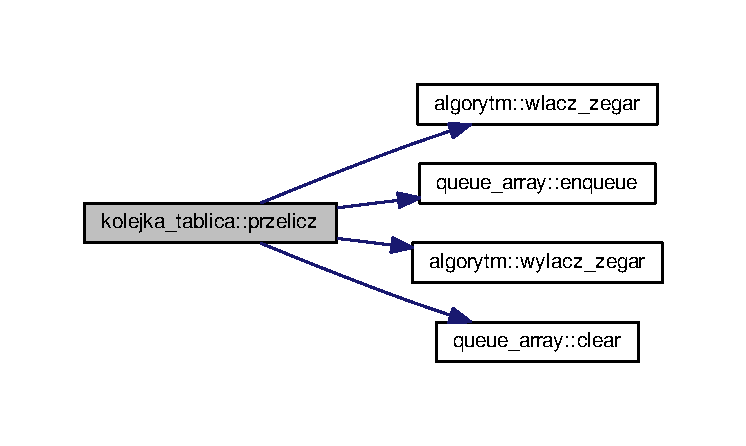
\includegraphics[width=350pt]{classkolejka__tablica_aad6baa28ce61111666e70df7d6ac4f86_cgraph}
\end{center}
\end{figure}




\subsection{Dokumentacja atrybutów składowych}
\hypertarget{classkolejka__tablica_a7fd15c7c7a0fa3649042ec634b2b8d4f}{\index{kolejka\-\_\-tablica@{kolejka\-\_\-tablica}!qu@{qu}}
\index{qu@{qu}!kolejka_tablica@{kolejka\-\_\-tablica}}
\subsubsection[{qu}]{\setlength{\rightskip}{0pt plus 5cm}{\bf queue\-\_\-array}$<$float$>$ kolejka\-\_\-tablica\-::qu\hspace{0.3cm}{\ttfamily [private]}}}\label{classkolejka__tablica_a7fd15c7c7a0fa3649042ec634b2b8d4f}


Definicja w linii 180 pliku algorytm.\-hh.



Dokumentacja dla tej klasy została wygenerowana z plików\-:\begin{DoxyCompactItemize}
\item 
\hyperlink{algorytm_8hh}{algorytm.\-hh}\item 
\hyperlink{algorytm_8cpp}{algorytm.\-cpp}\end{DoxyCompactItemize}

\hypertarget{classm__sort}{\section{\-Dokumentacja klasy m\-\_\-sort}
\label{classm__sort}\index{m\-\_\-sort@{m\-\_\-sort}}
}


klasa reprezentuje dane poddane sortowaniu przez scalanie  




{\ttfamily \#include $<$algorytm.\-hh$>$}



\-Diagram dziedziczenia dla m\-\_\-sort
\nopagebreak
\begin{figure}[H]
\begin{center}
\leavevmode
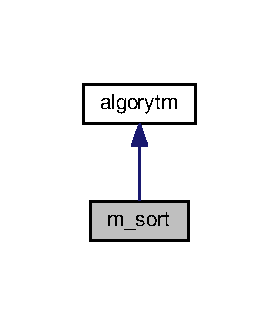
\includegraphics[width=134pt]{classm__sort__inherit__graph}
\end{center}
\end{figure}


\-Diagram współpracy dla m\-\_\-sort\-:
\nopagebreak
\begin{figure}[H]
\begin{center}
\leavevmode
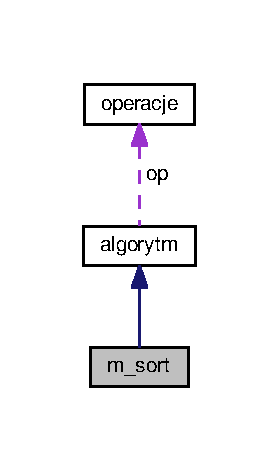
\includegraphics[width=134pt]{classm__sort__coll__graph}
\end{center}
\end{figure}
\subsection*{\-Metody publiczne}
\begin{DoxyCompactItemize}
\item 
\hyperlink{classm__sort_a9894abcd2ddd89f6963e80cc4038eed8}{m\-\_\-sort} (ifstream \&plik1, ifstream \&plik2, int \-N, int \-M)
\begin{DoxyCompactList}\small\item\em konstruktor \end{DoxyCompactList}\item 
float \hyperlink{classm__sort_acfcfa7bf26982bf718a169ccb771e694}{przelicz} ()
\begin{DoxyCompactList}\small\item\em metoda dokonujaca sortowania danych \end{DoxyCompactList}\end{DoxyCompactItemize}


\subsection{\-Opis szczegółowy}
klasa reprezentuje dane poddane sortowaniu przez scalanie 

\-Definicja w linii 212 pliku algorytm.\-hh.



\subsection{\-Dokumentacja konstruktora i destruktora}
\hypertarget{classm__sort_a9894abcd2ddd89f6963e80cc4038eed8}{\index{m\-\_\-sort@{m\-\_\-sort}!m\-\_\-sort@{m\-\_\-sort}}
\index{m\-\_\-sort@{m\-\_\-sort}!m_sort@{m\-\_\-sort}}
\subsubsection[{m\-\_\-sort}]{\setlength{\rightskip}{0pt plus 5cm}{\bf m\-\_\-sort\-::m\-\_\-sort} (
\begin{DoxyParamCaption}
\item[{ifstream \&}]{plik1, }
\item[{ifstream \&}]{plik2, }
\item[{int}]{\-N, }
\item[{int}]{\-M}
\end{DoxyParamCaption}
)\hspace{0.3cm}{\ttfamily  \mbox{[}inline\mbox{]}}}}\label{classm__sort_a9894abcd2ddd89f6963e80cc4038eed8}


konstruktor 



\-Definicja w linii 215 pliku algorytm.\-hh.



\subsection{\-Dokumentacja funkcji składowych}
\hypertarget{classm__sort_acfcfa7bf26982bf718a169ccb771e694}{\index{m\-\_\-sort@{m\-\_\-sort}!przelicz@{przelicz}}
\index{przelicz@{przelicz}!m_sort@{m\-\_\-sort}}
\subsubsection[{przelicz}]{\setlength{\rightskip}{0pt plus 5cm}float {\bf m\-\_\-sort\-::przelicz} (
\begin{DoxyParamCaption}
{}
\end{DoxyParamCaption}
)\hspace{0.3cm}{\ttfamily  \mbox{[}virtual\mbox{]}}}}\label{classm__sort_acfcfa7bf26982bf718a169ccb771e694}


metoda dokonujaca sortowania danych 



\-Reimplementowana z \hyperlink{classalgorytm_af3f92bf537b1f2e1f93173983e838449}{algorytm}.



\-Definicja w linii 183 pliku algorytm.\-cpp.



\-Oto graf wywołań dla tej funkcji\-:
\nopagebreak
\begin{figure}[H]
\begin{center}
\leavevmode
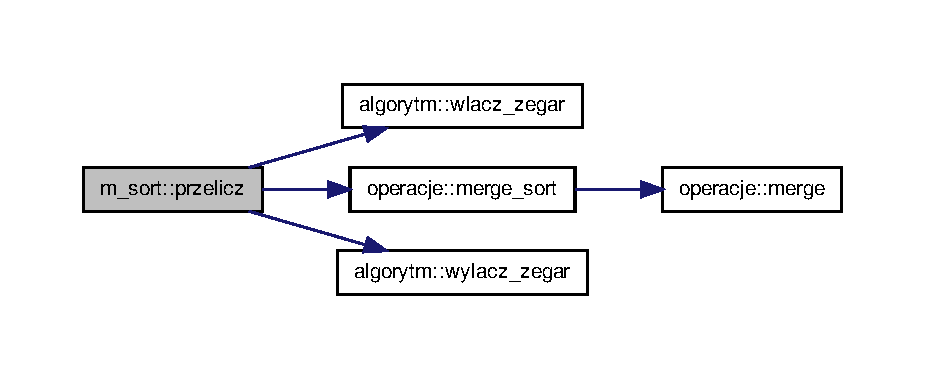
\includegraphics[width=350pt]{classm__sort_acfcfa7bf26982bf718a169ccb771e694_cgraph}
\end{center}
\end{figure}




\-Dokumentacja dla tej klasy została wygenerowana z plików\-:\begin{DoxyCompactItemize}
\item 
\hyperlink{algorytm_8hh}{algorytm.\-hh}\item 
\hyperlink{algorytm_8cpp}{algorytm.\-cpp}\end{DoxyCompactItemize}

\hypertarget{classmnozenie}{\section{\-Dokumentacja klasy mnozenie}
\label{classmnozenie}\index{mnozenie@{mnozenie}}
}


modeluje algorytm dokonujacy mnozenia kazdego elementu pliku wejsciowego przez 2  




{\ttfamily \#include $<$algorytm.\-hh$>$}



\-Diagram dziedziczenia dla mnozenie\nopagebreak
\begin{figure}[H]
\begin{center}
\leavevmode
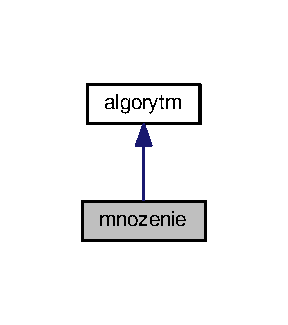
\includegraphics[width=138pt]{classmnozenie__inherit__graph}
\end{center}
\end{figure}


\-Diagram współpracy dla mnozenie\-:\nopagebreak
\begin{figure}[H]
\begin{center}
\leavevmode
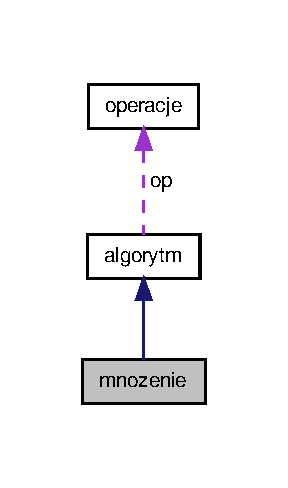
\includegraphics[width=138pt]{classmnozenie__coll__graph}
\end{center}
\end{figure}
\subsection*{\-Metody publiczne}
\begin{DoxyCompactItemize}
\item 
\hyperlink{classmnozenie_a105c483d60c621dc5c1855a04e285e3c}{mnozenie} (ifstream \&plik1, ifstream \&plik2, int \-N, int \-M)
\item 
void \hyperlink{classmnozenie_a5c97c36f9463bdf4eb7e34976a029930}{przelicz} ()
\begin{DoxyCompactList}\small\item\em wykonuje zalozony algorytm mnozenia elementow tablicy przez 2 \end{DoxyCompactList}\end{DoxyCompactItemize}


\subsection{\-Opis szczegółowy}
modeluje algorytm dokonujacy mnozenia kazdego elementu pliku wejsciowego przez 2 

\-Definicja w linii 125 pliku algorytm.\-hh.



\subsection{\-Dokumentacja konstruktora i destruktora}
\hypertarget{classmnozenie_a105c483d60c621dc5c1855a04e285e3c}{\index{mnozenie@{mnozenie}!mnozenie@{mnozenie}}
\index{mnozenie@{mnozenie}!mnozenie@{mnozenie}}
\subsubsection[{mnozenie}]{\setlength{\rightskip}{0pt plus 5cm}{\bf mnozenie\-::mnozenie} (
\begin{DoxyParamCaption}
\item[{ifstream \&}]{plik1, }
\item[{ifstream \&}]{plik2, }
\item[{int}]{\-N, }
\item[{int}]{\-M}
\end{DoxyParamCaption}
)\hspace{0.3cm}{\ttfamily  \mbox{[}inline\mbox{]}}}}\label{classmnozenie_a105c483d60c621dc5c1855a04e285e3c}
/brief konstruktor przekazuje do pol klasy informacje o nazwach pliku wejsciowego i wzorcowego 
\begin{DoxyParams}[1]{\-Parametry}
\mbox{\tt in}  & {\em plik1} & -\/ plik wejsciowy \\
\hline
\mbox{\tt in}  & {\em plik2} & -\/ plik wzorcowy \\
\hline
\mbox{\tt in}  & {\em \-N} & -\/ ilosc danych wejsciowych \\
\hline
\mbox{\tt in}  & {\em \-M} & -\/ ilosc powtorzen \\
\hline
\end{DoxyParams}


\-Definicja w linii 134 pliku algorytm.\-hh.



\subsection{\-Dokumentacja funkcji składowych}
\hypertarget{classmnozenie_a5c97c36f9463bdf4eb7e34976a029930}{\index{mnozenie@{mnozenie}!przelicz@{przelicz}}
\index{przelicz@{przelicz}!mnozenie@{mnozenie}}
\subsubsection[{przelicz}]{\setlength{\rightskip}{0pt plus 5cm}void {\bf mnozenie\-::przelicz} (
\begin{DoxyParamCaption}
{}
\end{DoxyParamCaption}
)\hspace{0.3cm}{\ttfamily  \mbox{[}virtual\mbox{]}}}}\label{classmnozenie_a5c97c36f9463bdf4eb7e34976a029930}


wykonuje zalozony algorytm mnozenia elementow tablicy przez 2 



\-Reimplementowana z \hyperlink{classalgorytm_aeefdd677ca8b9475a15547dcf8dd461f}{algorytm}.



\-Definicja w linii 81 pliku algorytm.\-cpp.



\-Dokumentacja dla tej klasy została wygenerowana z plików\-:\begin{DoxyCompactItemize}
\item 
\hyperlink{algorytm_8hh}{algorytm.\-hh}\item 
\hyperlink{algorytm_8cpp}{algorytm.\-cpp}\end{DoxyCompactItemize}

\hypertarget{classoperacje}{\section{\-Dokumentacja klasy operacje}
\label{classoperacje}\index{operacje@{operacje}}
}


\-Klasa modeluje tablice z danymi i metody sluzace do operacji na niej.  




{\ttfamily \#include $<$operacje.\-hh$>$}

\subsection*{\-Metody publiczne}
\begin{DoxyCompactItemize}
\item 
\hyperlink{classoperacje_a4538e0bfde26291449dc057134b23ad8}{operacje} ()
\begin{DoxyCompactList}\small\item\em konstruktor bezparametryczny \end{DoxyCompactList}\item 
\hyperlink{classoperacje_af109f7f9a4b10334d5e8c215c7f220de}{operacje} (int \-N)
\begin{DoxyCompactList}\small\item\em konstruktor parametryczny -\/ alokuje pamiec w dynamicznej tablicy {\ttfamily tab} \end{DoxyCompactList}\item 
bool \hyperlink{classoperacje_a7393a8b3b394921a084e0c1f4ad517b7}{zamien\-\_\-elementy} (int i, int j)
\begin{DoxyCompactList}\small\item\em \-Metoda zamienia 2 elementy tablicy. \end{DoxyCompactList}\item 
void \hyperlink{classoperacje_a7aa29c588e5a8f93c437150f03a133f1}{quick\-\_\-sort} (int l, int p)
\begin{DoxyCompactList}\small\item\em \-Metoda \-Dokonuje sortownaia szybkiego. \end{DoxyCompactList}\item 
void \hyperlink{classoperacje_a9be241905b909e7aef0151902c6f5b81}{make\-\_\-node} (int rozmiar, int i)
\begin{DoxyCompactList}\small\item\em \-Metoda tworzy wezel drzewa, przypisujac mu 2 synow, ustawiajac ich w odpowiedniej kolejnosci (ojciec ma najwieksza wartosc) \end{DoxyCompactList}\item 
void \hyperlink{classoperacje_ae752685beea6c7ee81d2347a98d40146}{make\-\_\-heap} ()
\begin{DoxyCompactList}\small\item\em \-Metoda tworzy kopiec binarny. \end{DoxyCompactList}\item 
void \hyperlink{classoperacje_aec9d2248eb072f97da794ee4c9b99a5d}{heap\-\_\-sort} ()
\begin{DoxyCompactList}\small\item\em \-Metoda dokonuje sortowania po uprzednim utworzeniu kopca. \end{DoxyCompactList}\item 
void \hyperlink{classoperacje_ad766f1d18595ff6b779485528c65d3f0}{merge} (int poczatek, int srodek, int koniec)
\begin{DoxyCompactList}\small\item\em \-Metoda scala dwie czesci tablicy, jednoczesnie je porzadkujac. \end{DoxyCompactList}\item 
void \hyperlink{classoperacje_ac65f2613b7d32b4f95e59bf2f8fd1aab}{merge\-\_\-sort} (int poczatek, int koniec)
\item 
void \hyperlink{classoperacje_aedc47c87f4f44f8af0cba64a940a5333}{odwroc\-\_\-tablice} ()
\begin{DoxyCompactList}\small\item\em metoda odwraca wszystkie elementy tablicy \end{DoxyCompactList}\item 
void \hyperlink{classoperacje_ad8397efded792c1381bfd0292b3e91b6}{dodaj\-\_\-element} (float e)
\begin{DoxyCompactList}\small\item\em metoda dodaje element do tablicy, alokujac dodatkowa pamiec \end{DoxyCompactList}\item 
void \hyperlink{classoperacje_a933533caa39434db543aca704804625c}{dodaj\-\_\-elementy} (float $\ast$tab2, int rozm)
\begin{DoxyCompactList}\small\item\em metoda dodaje elementy do tablicy \end{DoxyCompactList}\item 
void \hyperlink{classoperacje_a33127b613894949faba7a04f23075bf8}{operator=} (float $\ast$tab1)
\begin{DoxyCompactList}\small\item\em \-Przeciazenie operatora przypisania; przypisuje elementy tablicy {\ttfamily tab1} {\ttfamily do} tablicy bedacej polem klasy. \end{DoxyCompactList}\item 
bool \hyperlink{classoperacje_af69f25c4d1da5a7e46ff21a56143fc62}{operator==} (float $\ast$tab1)
\begin{DoxyCompactList}\small\item\em \-Przeciazenie operatora porownania; metoda porownuje zawartosci dwoch tablic. \end{DoxyCompactList}\item 
float \& \hyperlink{classoperacje_a6aeba674ecf3058e63e12bca9862a7fb}{operator\mbox{[}$\,$\mbox{]}} (int ind)
\end{DoxyCompactItemize}
\subsection*{\-Atrybuty publiczne}
\begin{DoxyCompactItemize}
\item 
int \hyperlink{classoperacje_aec7cc301d8822128d918aa1f9c7e1db2}{n}
\begin{DoxyCompactList}\small\item\em ilosc elementow w tablicy \end{DoxyCompactList}\item 
float $\ast$ \hyperlink{classoperacje_ad23bc418eebc9b493a5494ffd9358dd0}{tab}
\begin{DoxyCompactList}\small\item\em tablica z liczbami \end{DoxyCompactList}\end{DoxyCompactItemize}


\subsection{\-Opis szczegółowy}
\-Klasa modeluje tablice z danymi i metody sluzace do operacji na niej. 

\-Definicja w linii 11 pliku operacje.\-hh.



\subsection{\-Dokumentacja konstruktora i destruktora}
\hypertarget{classoperacje_a4538e0bfde26291449dc057134b23ad8}{\index{operacje@{operacje}!operacje@{operacje}}
\index{operacje@{operacje}!operacje@{operacje}}
\subsubsection[{operacje}]{\setlength{\rightskip}{0pt plus 5cm}{\bf operacje\-::operacje} (
\begin{DoxyParamCaption}
{}
\end{DoxyParamCaption}
)}}\label{classoperacje_a4538e0bfde26291449dc057134b23ad8}


konstruktor bezparametryczny 

\hypertarget{classoperacje_af109f7f9a4b10334d5e8c215c7f220de}{\index{operacje@{operacje}!operacje@{operacje}}
\index{operacje@{operacje}!operacje@{operacje}}
\subsubsection[{operacje}]{\setlength{\rightskip}{0pt plus 5cm}{\bf operacje\-::operacje} (
\begin{DoxyParamCaption}
\item[{int}]{\-N}
\end{DoxyParamCaption}
)\hspace{0.3cm}{\ttfamily  \mbox{[}inline\mbox{]}}}}\label{classoperacje_af109f7f9a4b10334d5e8c215c7f220de}


konstruktor parametryczny -\/ alokuje pamiec w dynamicznej tablicy {\ttfamily tab} 


\begin{DoxyParams}[1]{\-Parametry}
\mbox{\tt in}  & {\em \-N} & -\/ ilosc elementow w tablicy; parametr przypisywany do pola {\ttfamily n} w klasie, oraz alokuje pamiec o takim wlasnie rozmiarze \\
\hline
\end{DoxyParams}


\-Definicja w linii 28 pliku operacje.\-hh.



\subsection{\-Dokumentacja funkcji składowych}
\hypertarget{classoperacje_ad8397efded792c1381bfd0292b3e91b6}{\index{operacje@{operacje}!dodaj\-\_\-element@{dodaj\-\_\-element}}
\index{dodaj\-\_\-element@{dodaj\-\_\-element}!operacje@{operacje}}
\subsubsection[{dodaj\-\_\-element}]{\setlength{\rightskip}{0pt plus 5cm}void {\bf operacje\-::dodaj\-\_\-element} (
\begin{DoxyParamCaption}
\item[{float}]{e}
\end{DoxyParamCaption}
)}}\label{classoperacje_ad8397efded792c1381bfd0292b3e91b6}


metoda dodaje element do tablicy, alokujac dodatkowa pamiec 


\begin{DoxyParams}[1]{\-Parametry}
\mbox{\tt in}  & {\em e} & -\/ element, ktory nalezy dolaczyc do tablicy \\
\hline
\end{DoxyParams}


\-Definicja w linii 27 pliku operacje.\-cpp.

\hypertarget{classoperacje_a933533caa39434db543aca704804625c}{\index{operacje@{operacje}!dodaj\-\_\-elementy@{dodaj\-\_\-elementy}}
\index{dodaj\-\_\-elementy@{dodaj\-\_\-elementy}!operacje@{operacje}}
\subsubsection[{dodaj\-\_\-elementy}]{\setlength{\rightskip}{0pt plus 5cm}void {\bf operacje\-::dodaj\-\_\-elementy} (
\begin{DoxyParamCaption}
\item[{float $\ast$}]{tab2, }
\item[{int}]{rozm}
\end{DoxyParamCaption}
)}}\label{classoperacje_a933533caa39434db543aca704804625c}


metoda dodaje elementy do tablicy 


\begin{DoxyParams}[1]{\-Parametry}
\mbox{\tt in}  & {\em tab2} & -\/ tablica, ktora nalezy dolaczyc \\
\hline
\mbox{\tt in}  & {\em rozm} & -\/ rozmiar tablicy tab2 \\
\hline
\end{DoxyParams}


\-Definicja w linii 46 pliku operacje.\-cpp.

\hypertarget{classoperacje_aec9d2248eb072f97da794ee4c9b99a5d}{\index{operacje@{operacje}!heap\-\_\-sort@{heap\-\_\-sort}}
\index{heap\-\_\-sort@{heap\-\_\-sort}!operacje@{operacje}}
\subsubsection[{heap\-\_\-sort}]{\setlength{\rightskip}{0pt plus 5cm}void {\bf operacje\-::heap\-\_\-sort} (
\begin{DoxyParamCaption}
{}
\end{DoxyParamCaption}
)}}\label{classoperacje_aec9d2248eb072f97da794ee4c9b99a5d}


\-Metoda dokonuje sortowania po uprzednim utworzeniu kopca. 



\-Definicja w linii 116 pliku operacje.\-cpp.



\-Oto graf wywołań dla tej funkcji\-:\nopagebreak
\begin{figure}[H]
\begin{center}
\leavevmode
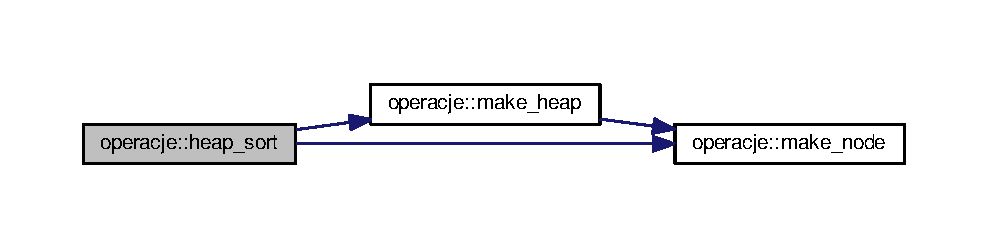
\includegraphics[width=350pt]{classoperacje_aec9d2248eb072f97da794ee4c9b99a5d_cgraph}
\end{center}
\end{figure}




\-Oto graf wywoływań tej funkcji\-:\nopagebreak
\begin{figure}[H]
\begin{center}
\leavevmode
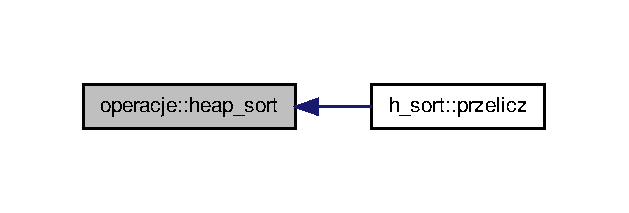
\includegraphics[width=302pt]{classoperacje_aec9d2248eb072f97da794ee4c9b99a5d_icgraph}
\end{center}
\end{figure}


\hypertarget{classoperacje_ae752685beea6c7ee81d2347a98d40146}{\index{operacje@{operacje}!make\-\_\-heap@{make\-\_\-heap}}
\index{make\-\_\-heap@{make\-\_\-heap}!operacje@{operacje}}
\subsubsection[{make\-\_\-heap}]{\setlength{\rightskip}{0pt plus 5cm}void {\bf operacje\-::make\-\_\-heap} (
\begin{DoxyParamCaption}
{}
\end{DoxyParamCaption}
)}}\label{classoperacje_ae752685beea6c7ee81d2347a98d40146}


\-Metoda tworzy kopiec binarny. 



\-Definicja w linii 110 pliku operacje.\-cpp.



\-Oto graf wywołań dla tej funkcji\-:\nopagebreak
\begin{figure}[H]
\begin{center}
\leavevmode
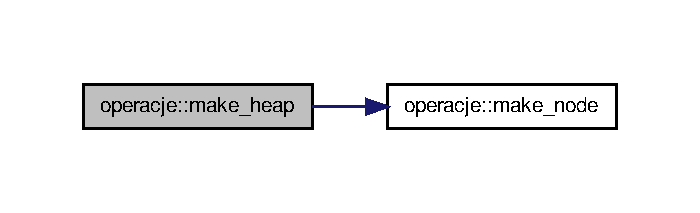
\includegraphics[width=336pt]{classoperacje_ae752685beea6c7ee81d2347a98d40146_cgraph}
\end{center}
\end{figure}




\-Oto graf wywoływań tej funkcji\-:\nopagebreak
\begin{figure}[H]
\begin{center}
\leavevmode
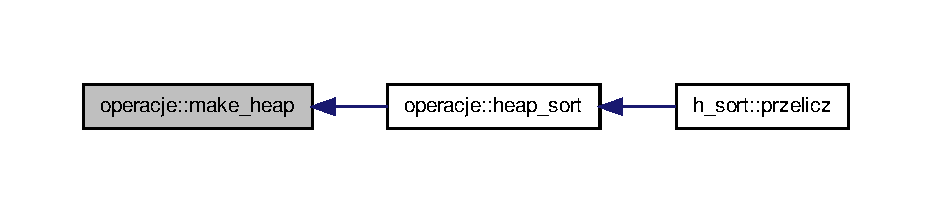
\includegraphics[width=350pt]{classoperacje_ae752685beea6c7ee81d2347a98d40146_icgraph}
\end{center}
\end{figure}


\hypertarget{classoperacje_a9be241905b909e7aef0151902c6f5b81}{\index{operacje@{operacje}!make\-\_\-node@{make\-\_\-node}}
\index{make\-\_\-node@{make\-\_\-node}!operacje@{operacje}}
\subsubsection[{make\-\_\-node}]{\setlength{\rightskip}{0pt plus 5cm}void {\bf operacje\-::make\-\_\-node} (
\begin{DoxyParamCaption}
\item[{int}]{rozmiar, }
\item[{int}]{i}
\end{DoxyParamCaption}
)}}\label{classoperacje_a9be241905b909e7aef0151902c6f5b81}


\-Metoda tworzy wezel drzewa, przypisujac mu 2 synow, ustawiajac ich w odpowiedniej kolejnosci (ojciec ma najwieksza wartosc) 


\begin{DoxyParams}[1]{\-Parametry}
\mbox{\tt in}  & {\em rozmiar} & -\/ rozmiar tablicy \\
\hline
\mbox{\tt in}  & {\em i} & -\/ indeks elementu, do ktorego przypisujemy synow \\
\hline
\end{DoxyParams}


\-Definicja w linii 95 pliku operacje.\-cpp.



\-Oto graf wywoływań tej funkcji\-:\nopagebreak
\begin{figure}[H]
\begin{center}
\leavevmode
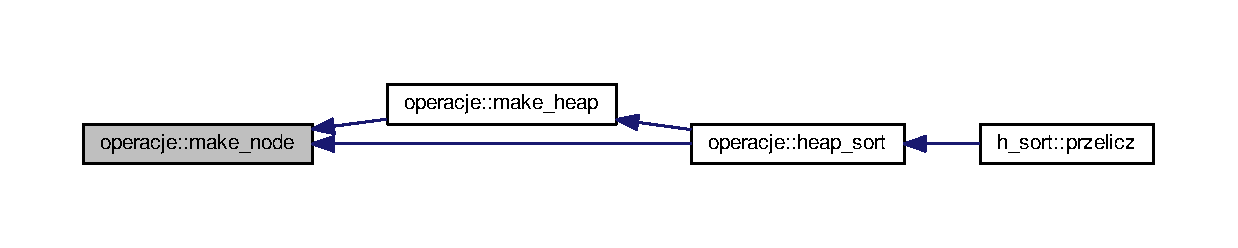
\includegraphics[width=350pt]{classoperacje_a9be241905b909e7aef0151902c6f5b81_icgraph}
\end{center}
\end{figure}


\hypertarget{classoperacje_ad766f1d18595ff6b779485528c65d3f0}{\index{operacje@{operacje}!merge@{merge}}
\index{merge@{merge}!operacje@{operacje}}
\subsubsection[{merge}]{\setlength{\rightskip}{0pt plus 5cm}void {\bf operacje\-::merge} (
\begin{DoxyParamCaption}
\item[{int}]{poczatek, }
\item[{int}]{srodek, }
\item[{int}]{koniec}
\end{DoxyParamCaption}
)}}\label{classoperacje_ad766f1d18595ff6b779485528c65d3f0}


\-Metoda scala dwie czesci tablicy, jednoczesnie je porzadkujac. 


\begin{DoxyParams}[1]{\-Parametry}
\mbox{\tt in}  & {\em poczatek} & -\/ pierwszy indeks tablicy \\
\hline
\mbox{\tt in}  & {\em srodek} & -\/ srodkowy indeks tablicy \\
\hline
\mbox{\tt in}  & {\em koniec} & -\/ ostatni indeks tablicy \\
\hline
\end{DoxyParams}


\-Definicja w linii 130 pliku operacje.\-cpp.



\-Oto graf wywoływań tej funkcji\-:\nopagebreak
\begin{figure}[H]
\begin{center}
\leavevmode
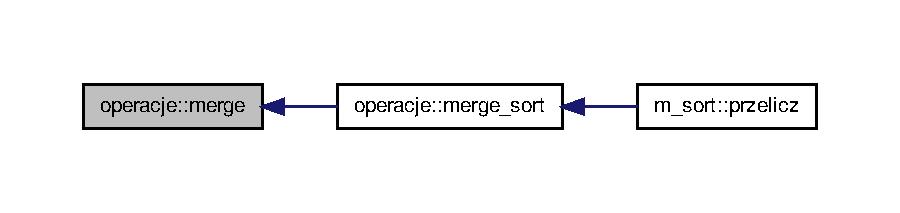
\includegraphics[width=350pt]{classoperacje_ad766f1d18595ff6b779485528c65d3f0_icgraph}
\end{center}
\end{figure}


\hypertarget{classoperacje_ac65f2613b7d32b4f95e59bf2f8fd1aab}{\index{operacje@{operacje}!merge\-\_\-sort@{merge\-\_\-sort}}
\index{merge\-\_\-sort@{merge\-\_\-sort}!operacje@{operacje}}
\subsubsection[{merge\-\_\-sort}]{\setlength{\rightskip}{0pt plus 5cm}void {\bf operacje\-::merge\-\_\-sort} (
\begin{DoxyParamCaption}
\item[{int}]{poczatek, }
\item[{int}]{koniec}
\end{DoxyParamCaption}
)}}\label{classoperacje_ac65f2613b7d32b4f95e59bf2f8fd1aab}
$\backslash$ brief \-Metoda dokonuje sortowania poprzez rekurencyjne wywolanie dla obu polow tablic, nastepnie metoda dokonuje scalenia danych 
\begin{DoxyParams}[1]{\-Parametry}
\mbox{\tt in}  & {\em poczatek} & -\/ pierwszy indeks tablicy \\
\hline
\mbox{\tt in}  & {\em koniec} & -\/ ostatni indeks tablicy \\
\hline
\end{DoxyParams}


\-Definicja w linii 166 pliku operacje.\-cpp.



\-Oto graf wywołań dla tej funkcji\-:\nopagebreak
\begin{figure}[H]
\begin{center}
\leavevmode
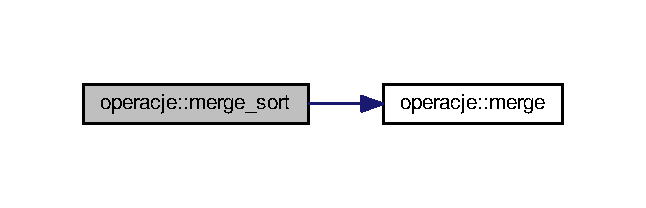
\includegraphics[width=310pt]{classoperacje_ac65f2613b7d32b4f95e59bf2f8fd1aab_cgraph}
\end{center}
\end{figure}




\-Oto graf wywoływań tej funkcji\-:\nopagebreak
\begin{figure}[H]
\begin{center}
\leavevmode
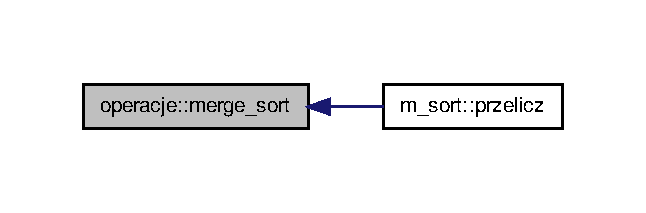
\includegraphics[width=310pt]{classoperacje_ac65f2613b7d32b4f95e59bf2f8fd1aab_icgraph}
\end{center}
\end{figure}


\hypertarget{classoperacje_aedc47c87f4f44f8af0cba64a940a5333}{\index{operacje@{operacje}!odwroc\-\_\-tablice@{odwroc\-\_\-tablice}}
\index{odwroc\-\_\-tablice@{odwroc\-\_\-tablice}!operacje@{operacje}}
\subsubsection[{odwroc\-\_\-tablice}]{\setlength{\rightskip}{0pt plus 5cm}void {\bf operacje\-::odwroc\-\_\-tablice} (
\begin{DoxyParamCaption}
{}
\end{DoxyParamCaption}
)}}\label{classoperacje_aedc47c87f4f44f8af0cba64a940a5333}


metoda odwraca wszystkie elementy tablicy 



\-Definicja w linii 12 pliku operacje.\-cpp.

\hypertarget{classoperacje_a33127b613894949faba7a04f23075bf8}{\index{operacje@{operacje}!operator=@{operator=}}
\index{operator=@{operator=}!operacje@{operacje}}
\subsubsection[{operator=}]{\setlength{\rightskip}{0pt plus 5cm}void operacje\-::operator= (
\begin{DoxyParamCaption}
\item[{float $\ast$}]{tab1}
\end{DoxyParamCaption}
)}}\label{classoperacje_a33127b613894949faba7a04f23075bf8}


\-Przeciazenie operatora przypisania; przypisuje elementy tablicy {\ttfamily tab1} {\ttfamily do} tablicy bedacej polem klasy. 


\begin{DoxyParams}[1]{\-Parametry}
\mbox{\tt in}  & {\em tab1} & -\/ tablica, ktorej zawartosc przypisujemy \\
\hline
\end{DoxyParams}


\-Definicja w linii 63 pliku operacje.\-cpp.

\hypertarget{classoperacje_af69f25c4d1da5a7e46ff21a56143fc62}{\index{operacje@{operacje}!operator==@{operator==}}
\index{operator==@{operator==}!operacje@{operacje}}
\subsubsection[{operator==}]{\setlength{\rightskip}{0pt plus 5cm}bool operacje\-::operator== (
\begin{DoxyParamCaption}
\item[{float $\ast$}]{tab1}
\end{DoxyParamCaption}
)}}\label{classoperacje_af69f25c4d1da5a7e46ff21a56143fc62}


\-Przeciazenie operatora porownania; metoda porownuje zawartosci dwoch tablic. 


\begin{DoxyParams}[1]{\-Parametry}
\mbox{\tt in}  & {\em tab1} & -\/ tablica, ktorej wartosci porownujemy \\
\hline
\end{DoxyParams}
\begin{DoxyReturn}{\-Zwraca}
true -\/ gdy zawartsoc tablic jest identyczna false -\/ w przeciwnym przypadku 
\end{DoxyReturn}


\-Definicja w linii 69 pliku operacje.\-cpp.

\hypertarget{classoperacje_a6aeba674ecf3058e63e12bca9862a7fb}{\index{operacje@{operacje}!operator\mbox{[}$\,$\mbox{]}@{operator[]}}
\index{operator\mbox{[}$\,$\mbox{]}@{operator[]}!operacje@{operacje}}
\subsubsection[{operator[]}]{\setlength{\rightskip}{0pt plus 5cm}float\& operacje\-::operator\mbox{[}$\,$\mbox{]} (
\begin{DoxyParamCaption}
\item[{int}]{ind}
\end{DoxyParamCaption}
)\hspace{0.3cm}{\ttfamily  \mbox{[}inline\mbox{]}}}}\label{classoperacje_a6aeba674ecf3058e63e12bca9862a7fb}


\-Definicja w linii 88 pliku operacje.\-hh.

\hypertarget{classoperacje_a7aa29c588e5a8f93c437150f03a133f1}{\index{operacje@{operacje}!quick\-\_\-sort@{quick\-\_\-sort}}
\index{quick\-\_\-sort@{quick\-\_\-sort}!operacje@{operacje}}
\subsubsection[{quick\-\_\-sort}]{\setlength{\rightskip}{0pt plus 5cm}void {\bf operacje\-::quick\-\_\-sort} (
\begin{DoxyParamCaption}
\item[{int}]{l, }
\item[{int}]{p}
\end{DoxyParamCaption}
)}}\label{classoperacje_a7aa29c588e5a8f93c437150f03a133f1}


\-Metoda \-Dokonuje sortownaia szybkiego. 


\begin{DoxyParams}[1]{\-Parametry}
\mbox{\tt in}  & {\em l} & -\/ pierwszy indeks tablicy \\
\hline
\mbox{\tt in}  & {\em p} & -\/ ostatni indeks tablicy \\
\hline
\end{DoxyParams}


\-Definicja w linii 77 pliku operacje.\-cpp.



\-Oto graf wywołań dla tej funkcji\-:\nopagebreak
\begin{figure}[H]
\begin{center}
\leavevmode
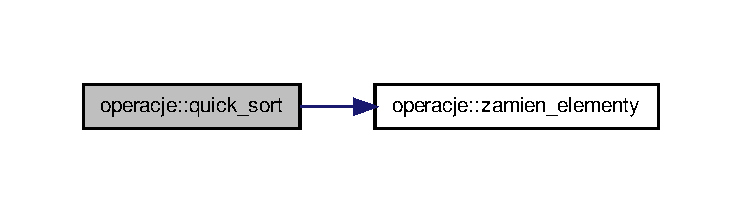
\includegraphics[width=350pt]{classoperacje_a7aa29c588e5a8f93c437150f03a133f1_cgraph}
\end{center}
\end{figure}




\-Oto graf wywoływań tej funkcji\-:\nopagebreak
\begin{figure}[H]
\begin{center}
\leavevmode
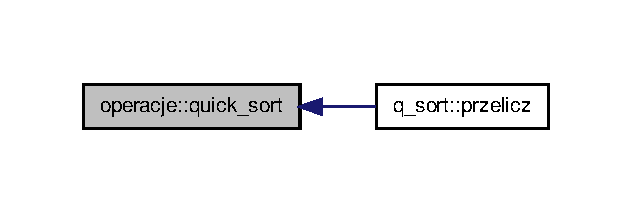
\includegraphics[width=304pt]{classoperacje_a7aa29c588e5a8f93c437150f03a133f1_icgraph}
\end{center}
\end{figure}


\hypertarget{classoperacje_a7393a8b3b394921a084e0c1f4ad517b7}{\index{operacje@{operacje}!zamien\-\_\-elementy@{zamien\-\_\-elementy}}
\index{zamien\-\_\-elementy@{zamien\-\_\-elementy}!operacje@{operacje}}
\subsubsection[{zamien\-\_\-elementy}]{\setlength{\rightskip}{0pt plus 5cm}bool {\bf operacje\-::zamien\-\_\-elementy} (
\begin{DoxyParamCaption}
\item[{int}]{i, }
\item[{int}]{j}
\end{DoxyParamCaption}
)}}\label{classoperacje_a7393a8b3b394921a084e0c1f4ad517b7}


\-Metoda zamienia 2 elementy tablicy. 


\begin{DoxyParams}[1]{\-Parametry}
\mbox{\tt in}  & {\em i} & -\/ element tablicy \\
\hline
\mbox{\tt in}  & {\em j} & -\/ element tablicy \\
\hline
\end{DoxyParams}
\begin{DoxyReturn}{\-Zwraca}
true -\/ gdy elementy nie wykraczaja poza zakres tablicy false -\/ w przeciwnym przypadku 
\end{DoxyReturn}


\-Definicja w linii 3 pliku operacje.\-cpp.



\-Oto graf wywoływań tej funkcji\-:\nopagebreak
\begin{figure}[H]
\begin{center}
\leavevmode
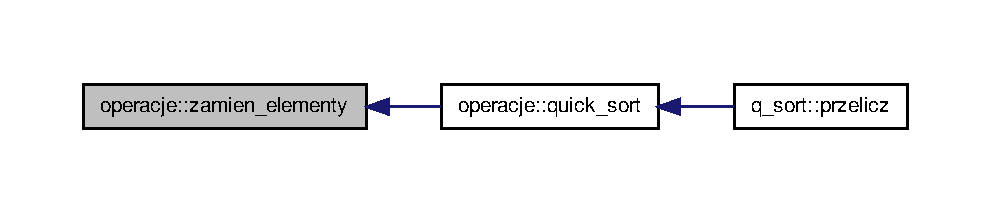
\includegraphics[width=350pt]{classoperacje_a7393a8b3b394921a084e0c1f4ad517b7_icgraph}
\end{center}
\end{figure}




\subsection{\-Dokumentacja atrybutów składowych}
\hypertarget{classoperacje_aec7cc301d8822128d918aa1f9c7e1db2}{\index{operacje@{operacje}!n@{n}}
\index{n@{n}!operacje@{operacje}}
\subsubsection[{n}]{\setlength{\rightskip}{0pt plus 5cm}int {\bf operacje\-::n}}}\label{classoperacje_aec7cc301d8822128d918aa1f9c7e1db2}


ilosc elementow w tablicy 



\-Definicja w linii 16 pliku operacje.\-hh.

\hypertarget{classoperacje_ad23bc418eebc9b493a5494ffd9358dd0}{\index{operacje@{operacje}!tab@{tab}}
\index{tab@{tab}!operacje@{operacje}}
\subsubsection[{tab}]{\setlength{\rightskip}{0pt plus 5cm}float$\ast$ {\bf operacje\-::tab}}}\label{classoperacje_ad23bc418eebc9b493a5494ffd9358dd0}


tablica z liczbami 



\-Definicja w linii 19 pliku operacje.\-hh.



\-Dokumentacja dla tej klasy została wygenerowana z plików\-:\begin{DoxyCompactItemize}
\item 
\hyperlink{operacje_8hh}{operacje.\-hh}\item 
\hyperlink{operacje_8cpp}{operacje.\-cpp}\end{DoxyCompactItemize}

\hypertarget{classq__sort}{\section{\-Dokumentacja klasy q\-\_\-sort}
\label{classq__sort}\index{q\-\_\-sort@{q\-\_\-sort}}
}


klasa reprezentuje dane poddane sortowaniu szybkiemu  




{\ttfamily \#include $<$algorytm.\-hh$>$}



\-Diagram dziedziczenia dla q\-\_\-sort
\nopagebreak
\begin{figure}[H]
\begin{center}
\leavevmode
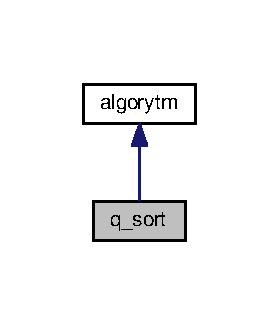
\includegraphics[width=134pt]{classq__sort__inherit__graph}
\end{center}
\end{figure}


\-Diagram współpracy dla q\-\_\-sort\-:
\nopagebreak
\begin{figure}[H]
\begin{center}
\leavevmode
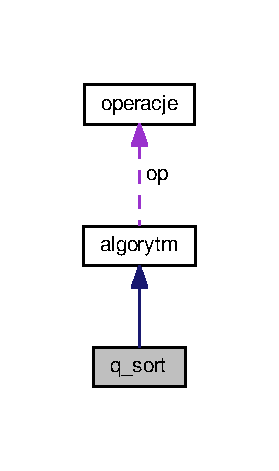
\includegraphics[width=134pt]{classq__sort__coll__graph}
\end{center}
\end{figure}
\subsection*{\-Metody publiczne}
\begin{DoxyCompactItemize}
\item 
\hyperlink{classq__sort_aeb7963f978713b880bbc19818752925d}{q\-\_\-sort} (ifstream \&plik1, ifstream \&plik2, int \-N, int \-M)
\begin{DoxyCompactList}\small\item\em konstruktor klasy \end{DoxyCompactList}\item 
float \hyperlink{classq__sort_a4f44405c764de7952fc0d821ef1206b5}{przelicz} ()
\begin{DoxyCompactList}\small\item\em metoda dokonujaca sortowania danych \end{DoxyCompactList}\end{DoxyCompactItemize}


\subsection{\-Opis szczegółowy}
klasa reprezentuje dane poddane sortowaniu szybkiemu 

\-Definicja w linii 195 pliku algorytm.\-hh.



\subsection{\-Dokumentacja konstruktora i destruktora}
\hypertarget{classq__sort_aeb7963f978713b880bbc19818752925d}{\index{q\-\_\-sort@{q\-\_\-sort}!q\-\_\-sort@{q\-\_\-sort}}
\index{q\-\_\-sort@{q\-\_\-sort}!q_sort@{q\-\_\-sort}}
\subsubsection[{q\-\_\-sort}]{\setlength{\rightskip}{0pt plus 5cm}{\bf q\-\_\-sort\-::q\-\_\-sort} (
\begin{DoxyParamCaption}
\item[{ifstream \&}]{plik1, }
\item[{ifstream \&}]{plik2, }
\item[{int}]{\-N, }
\item[{int}]{\-M}
\end{DoxyParamCaption}
)\hspace{0.3cm}{\ttfamily  \mbox{[}inline\mbox{]}}}}\label{classq__sort_aeb7963f978713b880bbc19818752925d}


konstruktor klasy 



\-Definicja w linii 198 pliku algorytm.\-hh.



\subsection{\-Dokumentacja funkcji składowych}
\hypertarget{classq__sort_a4f44405c764de7952fc0d821ef1206b5}{\index{q\-\_\-sort@{q\-\_\-sort}!przelicz@{przelicz}}
\index{przelicz@{przelicz}!q_sort@{q\-\_\-sort}}
\subsubsection[{przelicz}]{\setlength{\rightskip}{0pt plus 5cm}float {\bf q\-\_\-sort\-::przelicz} (
\begin{DoxyParamCaption}
{}
\end{DoxyParamCaption}
)\hspace{0.3cm}{\ttfamily  \mbox{[}virtual\mbox{]}}}}\label{classq__sort_a4f44405c764de7952fc0d821ef1206b5}


metoda dokonujaca sortowania danych 



\-Reimplementowana z \hyperlink{classalgorytm_af3f92bf537b1f2e1f93173983e838449}{algorytm}.



\-Definicja w linii 163 pliku algorytm.\-cpp.



\-Oto graf wywołań dla tej funkcji\-:
\nopagebreak
\begin{figure}[H]
\begin{center}
\leavevmode
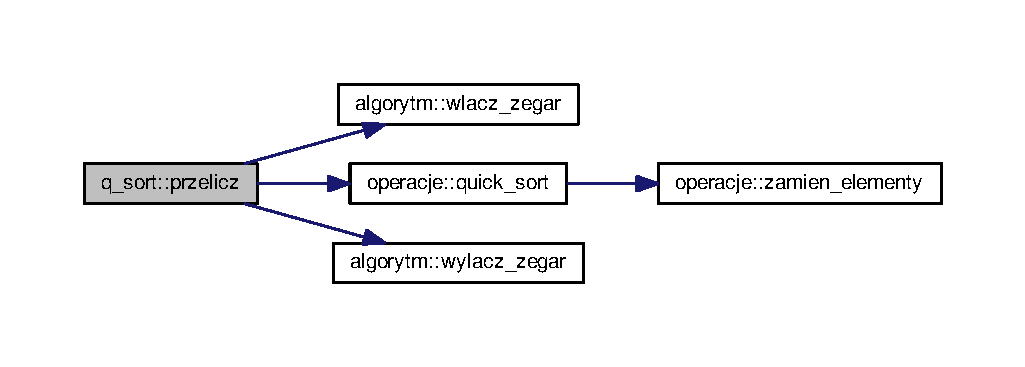
\includegraphics[width=350pt]{classq__sort_a4f44405c764de7952fc0d821ef1206b5_cgraph}
\end{center}
\end{figure}




\-Dokumentacja dla tej klasy została wygenerowana z plików\-:\begin{DoxyCompactItemize}
\item 
\hyperlink{algorytm_8hh}{algorytm.\-hh}\item 
\hyperlink{algorytm_8cpp}{algorytm.\-cpp}\end{DoxyCompactItemize}

\hypertarget{classqueue__array}{\section{Dokumentacja szablonu klasy queue\-\_\-array$<$ T\-Y\-P $>$}
\label{classqueue__array}\index{queue\-\_\-array$<$ T\-Y\-P $>$@{queue\-\_\-array$<$ T\-Y\-P $>$}}
}


Modeluje kolejke w oparciu o tablice.  




{\ttfamily \#include $<$kolejka.\-hh$>$}



Diagram współpracy dla queue\-\_\-array$<$ T\-Y\-P $>$\-:\nopagebreak
\begin{figure}[H]
\begin{center}
\leavevmode
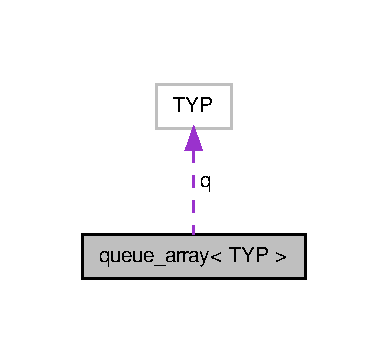
\includegraphics[width=186pt]{classqueue__array__coll__graph}
\end{center}
\end{figure}
\subsection*{Metody publiczne}
\begin{DoxyCompactItemize}
\item 
\hyperlink{classqueue__array_af651ba1c08e777af1ef23d1301819c58}{queue\-\_\-array} ()
\begin{DoxyCompactList}\small\item\em konstruktor bezparametryczny \end{DoxyCompactList}\item 
\hyperlink{classqueue__array_ad2c9f7906fad18d3daad605455210cb8}{queue\-\_\-array} (\hyperlink{stos_8hh_a7847560c748814fd3070e9149a9578bd}{flag} F)
\begin{DoxyCompactList}\small\item\em konstruktor parametryczny -\/ ustawia flage na zadana pozycje \end{DoxyCompactList}\item 
int \hyperlink{classqueue__array_a423093872e5cf4eb99f17ca1179ffa70}{size} ()
\item 
bool \hyperlink{classqueue__array_aa6ddf8e684f31a34f721e89ea83a7469}{is\-\_\-empty} ()
\item 
void \hyperlink{classqueue__array_a0c35f63c53ee3e3019fffde84bbf6bd1}{enqueue} (T\-Y\-P element)
\begin{DoxyCompactList}\small\item\em Dodaje element na poczatek kolejki w zaleznosci od wybranego trybu powiekszania tablicy. \end{DoxyCompactList}\item 
T\-Y\-P \hyperlink{classqueue__array_a67a036da416c976652c9039e5e101538}{dequeue} ()
\begin{DoxyCompactList}\small\item\em usuwa element z konca kolejki \end{DoxyCompactList}\item 
void \hyperlink{classqueue__array_acfe3b3e3ed5cc3b380d3f0d261ade3d9}{clear} ()
\begin{DoxyCompactList}\small\item\em czysci kolejke \end{DoxyCompactList}\end{DoxyCompactItemize}
\subsection*{Atrybuty publiczne}
\begin{DoxyCompactItemize}
\item 
\hyperlink{stos_8hh_a7847560c748814fd3070e9149a9578bd}{flag} \hyperlink{classqueue__array_a01c734086cf5e56c719b4d327cc36664}{f}
\begin{DoxyCompactList}\small\item\em flaga trybu zwiekszania pamieci , przyjmuje wartosc \-: plus1 -\/ dla trybu kazdorazowego powiekszania pamieci x2 -\/ dla trybu podwajania rozmiaru struktury \end{DoxyCompactList}\end{DoxyCompactItemize}
\subsection*{Atrybuty prywatne}
\begin{DoxyCompactItemize}
\item 
T\-Y\-P $\ast$ \hyperlink{classqueue__array_a073323517389c0d97534b90682317ce3}{q}
\item 
int \hyperlink{classqueue__array_a87d275726c2f69acb8ea9f0b3ab899f6}{s}
\item 
int \hyperlink{classqueue__array_a94cdc73c1df75d4fe0c75a852528cde9}{sp}
\end{DoxyCompactItemize}


\subsection{Opis szczegółowy}
\subsubsection*{template$<$typename T\-Y\-P$>$class queue\-\_\-array$<$ T\-Y\-P $>$}

Modeluje kolejke w oparciu o tablice. 

Definicja w linii 50 pliku kolejka.\-hh.



\subsection{Dokumentacja konstruktora i destruktora}
\hypertarget{classqueue__array_af651ba1c08e777af1ef23d1301819c58}{\index{queue\-\_\-array@{queue\-\_\-array}!queue\-\_\-array@{queue\-\_\-array}}
\index{queue\-\_\-array@{queue\-\_\-array}!queue_array@{queue\-\_\-array}}
\subsubsection[{queue\-\_\-array}]{\setlength{\rightskip}{0pt plus 5cm}template$<$typename T\-Y\-P$>$ {\bf queue\-\_\-array}$<$ T\-Y\-P $>$\-::{\bf queue\-\_\-array} (
\begin{DoxyParamCaption}
{}
\end{DoxyParamCaption}
)\hspace{0.3cm}{\ttfamily [inline]}}}\label{classqueue__array_af651ba1c08e777af1ef23d1301819c58}


konstruktor bezparametryczny 



Definicja w linii 63 pliku kolejka.\-hh.

\hypertarget{classqueue__array_ad2c9f7906fad18d3daad605455210cb8}{\index{queue\-\_\-array@{queue\-\_\-array}!queue\-\_\-array@{queue\-\_\-array}}
\index{queue\-\_\-array@{queue\-\_\-array}!queue_array@{queue\-\_\-array}}
\subsubsection[{queue\-\_\-array}]{\setlength{\rightskip}{0pt plus 5cm}template$<$typename T\-Y\-P$>$ {\bf queue\-\_\-array}$<$ T\-Y\-P $>$\-::{\bf queue\-\_\-array} (
\begin{DoxyParamCaption}
\item[{{\bf flag}}]{F}
\end{DoxyParamCaption}
)\hspace{0.3cm}{\ttfamily [inline]}}}\label{classqueue__array_ad2c9f7906fad18d3daad605455210cb8}


konstruktor parametryczny -\/ ustawia flage na zadana pozycje 



Definicja w linii 65 pliku kolejka.\-hh.



\subsection{Dokumentacja funkcji składowych}
\hypertarget{classqueue__array_acfe3b3e3ed5cc3b380d3f0d261ade3d9}{\index{queue\-\_\-array@{queue\-\_\-array}!clear@{clear}}
\index{clear@{clear}!queue_array@{queue\-\_\-array}}
\subsubsection[{clear}]{\setlength{\rightskip}{0pt plus 5cm}template$<$typename T\-Y\-P$>$ void {\bf queue\-\_\-array}$<$ T\-Y\-P $>$\-::clear (
\begin{DoxyParamCaption}
{}
\end{DoxyParamCaption}
)\hspace{0.3cm}{\ttfamily [inline]}}}\label{classqueue__array_acfe3b3e3ed5cc3b380d3f0d261ade3d9}


czysci kolejke 



Definicja w linii 173 pliku kolejka.\-hh.



Oto graf wywoływań tej funkcji\-:\nopagebreak
\begin{figure}[H]
\begin{center}
\leavevmode
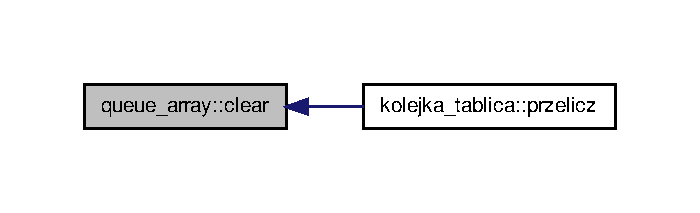
\includegraphics[width=336pt]{classqueue__array_acfe3b3e3ed5cc3b380d3f0d261ade3d9_icgraph}
\end{center}
\end{figure}


\hypertarget{classqueue__array_a67a036da416c976652c9039e5e101538}{\index{queue\-\_\-array@{queue\-\_\-array}!dequeue@{dequeue}}
\index{dequeue@{dequeue}!queue_array@{queue\-\_\-array}}
\subsubsection[{dequeue}]{\setlength{\rightskip}{0pt plus 5cm}template$<$typename T\-Y\-P$>$ T\-Y\-P {\bf queue\-\_\-array}$<$ T\-Y\-P $>$\-::dequeue (
\begin{DoxyParamCaption}
{}
\end{DoxyParamCaption}
)\hspace{0.3cm}{\ttfamily [inline]}}}\label{classqueue__array_a67a036da416c976652c9039e5e101538}


usuwa element z konca kolejki 



Definicja w linii 129 pliku kolejka.\-hh.



Oto graf wywoływań tej funkcji\-:\nopagebreak
\begin{figure}[H]
\begin{center}
\leavevmode
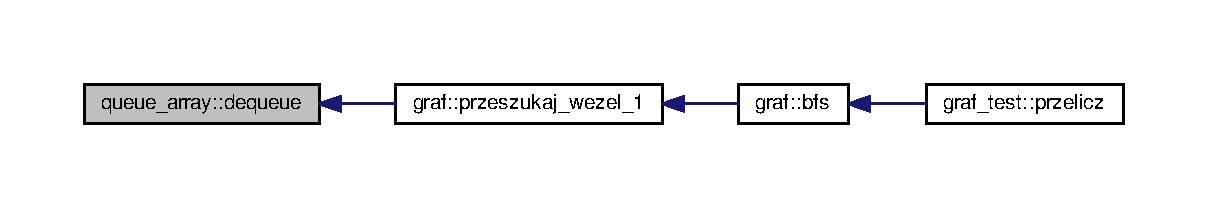
\includegraphics[width=350pt]{classqueue__array_a67a036da416c976652c9039e5e101538_icgraph}
\end{center}
\end{figure}


\hypertarget{classqueue__array_a0c35f63c53ee3e3019fffde84bbf6bd1}{\index{queue\-\_\-array@{queue\-\_\-array}!enqueue@{enqueue}}
\index{enqueue@{enqueue}!queue_array@{queue\-\_\-array}}
\subsubsection[{enqueue}]{\setlength{\rightskip}{0pt plus 5cm}template$<$typename T\-Y\-P$>$ void {\bf queue\-\_\-array}$<$ T\-Y\-P $>$\-::enqueue (
\begin{DoxyParamCaption}
\item[{T\-Y\-P}]{element}
\end{DoxyParamCaption}
)\hspace{0.3cm}{\ttfamily [inline]}}}\label{classqueue__array_a0c35f63c53ee3e3019fffde84bbf6bd1}


Dodaje element na poczatek kolejki w zaleznosci od wybranego trybu powiekszania tablicy. 



Definicja w linii 82 pliku kolejka.\-hh.



Oto graf wywoływań tej funkcji\-:\nopagebreak
\begin{figure}[H]
\begin{center}
\leavevmode
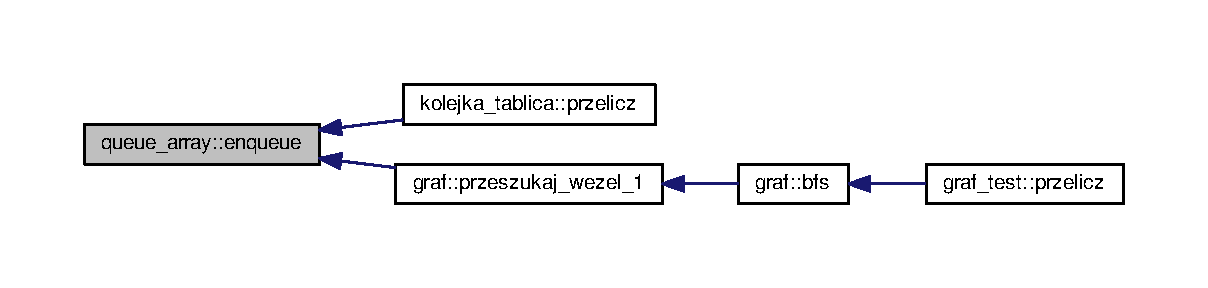
\includegraphics[width=350pt]{classqueue__array_a0c35f63c53ee3e3019fffde84bbf6bd1_icgraph}
\end{center}
\end{figure}


\hypertarget{classqueue__array_aa6ddf8e684f31a34f721e89ea83a7469}{\index{queue\-\_\-array@{queue\-\_\-array}!is\-\_\-empty@{is\-\_\-empty}}
\index{is\-\_\-empty@{is\-\_\-empty}!queue_array@{queue\-\_\-array}}
\subsubsection[{is\-\_\-empty}]{\setlength{\rightskip}{0pt plus 5cm}template$<$typename T\-Y\-P$>$ bool {\bf queue\-\_\-array}$<$ T\-Y\-P $>$\-::is\-\_\-empty (
\begin{DoxyParamCaption}
{}
\end{DoxyParamCaption}
)\hspace{0.3cm}{\ttfamily [inline]}}}\label{classqueue__array_aa6ddf8e684f31a34f721e89ea83a7469}
\begin{DoxyReturn}{Zwraca}
false -\/ gdy kolejka nie jest pusta, true , gdy pusta 
\end{DoxyReturn}


Definicja w linii 75 pliku kolejka.\-hh.



Oto graf wywoływań tej funkcji\-:\nopagebreak
\begin{figure}[H]
\begin{center}
\leavevmode
\includegraphics[width=350pt]{classqueue__array_aa6ddf8e684f31a34f721e89ea83a7469_icgraph}
\end{center}
\end{figure}


\hypertarget{classqueue__array_a423093872e5cf4eb99f17ca1179ffa70}{\index{queue\-\_\-array@{queue\-\_\-array}!size@{size}}
\index{size@{size}!queue_array@{queue\-\_\-array}}
\subsubsection[{size}]{\setlength{\rightskip}{0pt plus 5cm}template$<$typename T\-Y\-P$>$ int {\bf queue\-\_\-array}$<$ T\-Y\-P $>$\-::size (
\begin{DoxyParamCaption}
{}
\end{DoxyParamCaption}
)\hspace{0.3cm}{\ttfamily [inline]}}}\label{classqueue__array_a423093872e5cf4eb99f17ca1179ffa70}
\begin{DoxyReturn}{Zwraca}
rozmiar kolejki 
\end{DoxyReturn}


Definicja w linii 70 pliku kolejka.\-hh.



\subsection{Dokumentacja atrybutów składowych}
\hypertarget{classqueue__array_a01c734086cf5e56c719b4d327cc36664}{\index{queue\-\_\-array@{queue\-\_\-array}!f@{f}}
\index{f@{f}!queue_array@{queue\-\_\-array}}
\subsubsection[{f}]{\setlength{\rightskip}{0pt plus 5cm}template$<$typename T\-Y\-P$>$ {\bf flag} {\bf queue\-\_\-array}$<$ T\-Y\-P $>$\-::f}}\label{classqueue__array_a01c734086cf5e56c719b4d327cc36664}


flaga trybu zwiekszania pamieci , przyjmuje wartosc \-: plus1 -\/ dla trybu kazdorazowego powiekszania pamieci x2 -\/ dla trybu podwajania rozmiaru struktury 



Definicja w linii 59 pliku kolejka.\-hh.

\hypertarget{classqueue__array_a073323517389c0d97534b90682317ce3}{\index{queue\-\_\-array@{queue\-\_\-array}!q@{q}}
\index{q@{q}!queue_array@{queue\-\_\-array}}
\subsubsection[{q}]{\setlength{\rightskip}{0pt plus 5cm}template$<$typename T\-Y\-P$>$ T\-Y\-P$\ast$ {\bf queue\-\_\-array}$<$ T\-Y\-P $>$\-::q\hspace{0.3cm}{\ttfamily [private]}}}\label{classqueue__array_a073323517389c0d97534b90682317ce3}


Definicja w linii 51 pliku kolejka.\-hh.

\hypertarget{classqueue__array_a87d275726c2f69acb8ea9f0b3ab899f6}{\index{queue\-\_\-array@{queue\-\_\-array}!s@{s}}
\index{s@{s}!queue_array@{queue\-\_\-array}}
\subsubsection[{s}]{\setlength{\rightskip}{0pt plus 5cm}template$<$typename T\-Y\-P$>$ int {\bf queue\-\_\-array}$<$ T\-Y\-P $>$\-::s\hspace{0.3cm}{\ttfamily [private]}}}\label{classqueue__array_a87d275726c2f69acb8ea9f0b3ab899f6}


Definicja w linii 52 pliku kolejka.\-hh.

\hypertarget{classqueue__array_a94cdc73c1df75d4fe0c75a852528cde9}{\index{queue\-\_\-array@{queue\-\_\-array}!sp@{sp}}
\index{sp@{sp}!queue_array@{queue\-\_\-array}}
\subsubsection[{sp}]{\setlength{\rightskip}{0pt plus 5cm}template$<$typename T\-Y\-P$>$ int {\bf queue\-\_\-array}$<$ T\-Y\-P $>$\-::sp\hspace{0.3cm}{\ttfamily [private]}}}\label{classqueue__array_a94cdc73c1df75d4fe0c75a852528cde9}


Definicja w linii 52 pliku kolejka.\-hh.



Dokumentacja dla tej klasy została wygenerowana z pliku\-:\begin{DoxyCompactItemize}
\item 
\hyperlink{kolejka_8hh}{kolejka.\-hh}\end{DoxyCompactItemize}

\hypertarget{classqueue__list}{\section{\-Dokumentacja szablonu klasy queue\-\_\-list$<$ \-T\-Y\-P $>$}
\label{classqueue__list}\index{queue\-\_\-list$<$ T\-Y\-P $>$@{queue\-\_\-list$<$ T\-Y\-P $>$}}
}


\-Modeluje kolejke oparta na liscie \-S\-T\-L.  




{\ttfamily \#include $<$kolejka.\-hh$>$}

\subsection*{\-Metody publiczne}
\begin{DoxyCompactItemize}
\item 
bool \hyperlink{classqueue__list_a762d9f9f56dc9552e8df07d1b732e8b0}{is\-\_\-empty} ()
\item 
int \hyperlink{classqueue__list_aa9d1aaf18cca43fcee4e0a0dfb212cd4}{size} ()
\item 
void \hyperlink{classqueue__list_ab2985d4f0192202336311fd89d836573}{enqueue} (\-T\-Y\-P \&element)
\begin{DoxyCompactList}\small\item\em dodaje element \end{DoxyCompactList}\item 
\-T\-Y\-P \hyperlink{classqueue__list_add17ee76e80f7e09cc470ba55bd4c131}{dequeue} ()
\begin{DoxyCompactList}\small\item\em usuwa element \end{DoxyCompactList}\item 
void \hyperlink{classqueue__list_a4dcb6bb4dfee45fb084dff647ded82f0}{clear} ()
\begin{DoxyCompactList}\small\item\em czysci stos \end{DoxyCompactList}\end{DoxyCompactItemize}
\subsection*{\-Atrybuty prywatne}
\begin{DoxyCompactItemize}
\item 
list$<$ \-T\-Y\-P $>$ \hyperlink{classqueue__list_a452a11e2c4872ff7b6622d06e6d01c98}{q}
\end{DoxyCompactItemize}


\subsection{\-Opis szczegółowy}
\subsubsection*{template$<$typename \-T\-Y\-P$>$class queue\-\_\-list$<$ T\-Y\-P $>$}

\-Modeluje kolejke oparta na liscie \-S\-T\-L. 

\-Definicja w linii 19 pliku kolejka.\-hh.



\subsection{\-Dokumentacja funkcji składowych}
\hypertarget{classqueue__list_a4dcb6bb4dfee45fb084dff647ded82f0}{\index{queue\-\_\-list@{queue\-\_\-list}!clear@{clear}}
\index{clear@{clear}!queue_list@{queue\-\_\-list}}
\subsubsection[{clear}]{\setlength{\rightskip}{0pt plus 5cm}template$<$typename \-T\-Y\-P$>$ void {\bf queue\-\_\-list}$<$ \-T\-Y\-P $>$\-::{\bf clear} (
\begin{DoxyParamCaption}
{}
\end{DoxyParamCaption}
)\hspace{0.3cm}{\ttfamily  \mbox{[}inline\mbox{]}}}}\label{classqueue__list_a4dcb6bb4dfee45fb084dff647ded82f0}


czysci stos 



\-Definicja w linii 41 pliku kolejka.\-hh.



\-Oto graf wywoływań tej funkcji\-:\nopagebreak
\begin{figure}[H]
\begin{center}
\leavevmode
\includegraphics[width=314pt]{classqueue__list_a4dcb6bb4dfee45fb084dff647ded82f0_icgraph}
\end{center}
\end{figure}


\hypertarget{classqueue__list_add17ee76e80f7e09cc470ba55bd4c131}{\index{queue\-\_\-list@{queue\-\_\-list}!dequeue@{dequeue}}
\index{dequeue@{dequeue}!queue_list@{queue\-\_\-list}}
\subsubsection[{dequeue}]{\setlength{\rightskip}{0pt plus 5cm}template$<$typename \-T\-Y\-P$>$ \-T\-Y\-P {\bf queue\-\_\-list}$<$ \-T\-Y\-P $>$\-::{\bf dequeue} (
\begin{DoxyParamCaption}
{}
\end{DoxyParamCaption}
)\hspace{0.3cm}{\ttfamily  \mbox{[}inline\mbox{]}}}}\label{classqueue__list_add17ee76e80f7e09cc470ba55bd4c131}


usuwa element 



\-Definicja w linii 35 pliku kolejka.\-hh.

\hypertarget{classqueue__list_ab2985d4f0192202336311fd89d836573}{\index{queue\-\_\-list@{queue\-\_\-list}!enqueue@{enqueue}}
\index{enqueue@{enqueue}!queue_list@{queue\-\_\-list}}
\subsubsection[{enqueue}]{\setlength{\rightskip}{0pt plus 5cm}template$<$typename \-T\-Y\-P$>$ void {\bf queue\-\_\-list}$<$ \-T\-Y\-P $>$\-::{\bf enqueue} (
\begin{DoxyParamCaption}
\item[{\-T\-Y\-P \&}]{element}
\end{DoxyParamCaption}
)\hspace{0.3cm}{\ttfamily  \mbox{[}inline\mbox{]}}}}\label{classqueue__list_ab2985d4f0192202336311fd89d836573}


dodaje element 



\-Definicja w linii 33 pliku kolejka.\-hh.



\-Oto graf wywoływań tej funkcji\-:\nopagebreak
\begin{figure}[H]
\begin{center}
\leavevmode
\includegraphics[width=330pt]{classqueue__list_ab2985d4f0192202336311fd89d836573_icgraph}
\end{center}
\end{figure}


\hypertarget{classqueue__list_a762d9f9f56dc9552e8df07d1b732e8b0}{\index{queue\-\_\-list@{queue\-\_\-list}!is\-\_\-empty@{is\-\_\-empty}}
\index{is\-\_\-empty@{is\-\_\-empty}!queue_list@{queue\-\_\-list}}
\subsubsection[{is\-\_\-empty}]{\setlength{\rightskip}{0pt plus 5cm}template$<$typename \-T\-Y\-P$>$ bool {\bf queue\-\_\-list}$<$ \-T\-Y\-P $>$\-::{\bf is\-\_\-empty} (
\begin{DoxyParamCaption}
{}
\end{DoxyParamCaption}
)\hspace{0.3cm}{\ttfamily  \mbox{[}inline\mbox{]}}}}\label{classqueue__list_a762d9f9f56dc9552e8df07d1b732e8b0}
\begin{DoxyReturn}{\-Zwraca}
false -\/ gdy kolejka nie jest pusta, true , gdy pusta 
\end{DoxyReturn}


\-Definicja w linii 26 pliku kolejka.\-hh.

\hypertarget{classqueue__list_aa9d1aaf18cca43fcee4e0a0dfb212cd4}{\index{queue\-\_\-list@{queue\-\_\-list}!size@{size}}
\index{size@{size}!queue_list@{queue\-\_\-list}}
\subsubsection[{size}]{\setlength{\rightskip}{0pt plus 5cm}template$<$typename \-T\-Y\-P$>$ int {\bf queue\-\_\-list}$<$ \-T\-Y\-P $>$\-::{\bf size} (
\begin{DoxyParamCaption}
{}
\end{DoxyParamCaption}
)\hspace{0.3cm}{\ttfamily  \mbox{[}inline\mbox{]}}}}\label{classqueue__list_aa9d1aaf18cca43fcee4e0a0dfb212cd4}
\begin{DoxyReturn}{\-Zwraca}
rozmiar kolejki 
\end{DoxyReturn}


\-Definicja w linii 31 pliku kolejka.\-hh.



\subsection{\-Dokumentacja atrybutów składowych}
\hypertarget{classqueue__list_a452a11e2c4872ff7b6622d06e6d01c98}{\index{queue\-\_\-list@{queue\-\_\-list}!q@{q}}
\index{q@{q}!queue_list@{queue\-\_\-list}}
\subsubsection[{q}]{\setlength{\rightskip}{0pt plus 5cm}template$<$typename \-T\-Y\-P$>$ list$<$\-T\-Y\-P$>$ {\bf queue\-\_\-list}$<$ \-T\-Y\-P $>$\-::{\bf q}\hspace{0.3cm}{\ttfamily  \mbox{[}private\mbox{]}}}}\label{classqueue__list_a452a11e2c4872ff7b6622d06e6d01c98}


\-Definicja w linii 20 pliku kolejka.\-hh.



\-Dokumentacja dla tej klasy została wygenerowana z pliku\-:\begin{DoxyCompactItemize}
\item 
\hyperlink{kolejka_8hh}{kolejka.\-hh}\end{DoxyCompactItemize}

\hypertarget{classstack__array}{\section{\-Dokumentacja szablonu klasy stack\-\_\-array$<$ \-T\-Y\-P $>$}
\label{classstack__array}\index{stack\-\_\-array$<$ T\-Y\-P $>$@{stack\-\_\-array$<$ T\-Y\-P $>$}}
}


\-Modeluje stos w oparciu o tablice.  




{\ttfamily \#include $<$stos.\-hh$>$}



\-Diagram współpracy dla stack\-\_\-array$<$ \-T\-Y\-P $>$\-:\nopagebreak
\begin{figure}[H]
\begin{center}
\leavevmode
\includegraphics[width=184pt]{classstack__array__coll__graph}
\end{center}
\end{figure}
\subsection*{\-Metody publiczne}
\begin{DoxyCompactItemize}
\item 
\hyperlink{classstack__array_a430ec07ba59152bdb618039ae5f74482}{stack\-\_\-array} ()
\begin{DoxyCompactList}\small\item\em konstruktor bezparametryczny \end{DoxyCompactList}\item 
\hyperlink{classstack__array_ad6ac30696a594fc1f4b58cc94facad9f}{stack\-\_\-array} (\hyperlink{stos_8hh_a7847560c748814fd3070e9149a9578bd}{flag} \-F)
\begin{DoxyCompactList}\small\item\em konstruktor parametryczny -\/ ustawia flage na zadana pozycje \end{DoxyCompactList}\item 
bool \hyperlink{classstack__array_a653b67eb0566e9481e3525dd2f2bc519}{is\-\_\-empty} ()
\item 
int \hyperlink{classstack__array_a26ee4c653f299d3fe03b443f6180d745}{size} ()
\item 
void \hyperlink{classstack__array_a2f48529c5e88d82f5da2b27c945e1b0e}{push} (\-T\-Y\-P \&element)
\begin{DoxyCompactList}\small\item\em \-Dodaje element na wierzch stosu w zaleznosci od wybranego trybu powiekszania tablicy. \end{DoxyCompactList}\item 
\-T\-Y\-P \hyperlink{classstack__array_ad2ce52b1a99f72d383b429dff262b9eb}{pop} ()
\begin{DoxyCompactList}\small\item\em zdejmuje element ze stosu \end{DoxyCompactList}\item 
void \hyperlink{classstack__array_ac55f6fe35d44781d918884e4c466d3ee}{clear} ()
\begin{DoxyCompactList}\small\item\em czysci stos \end{DoxyCompactList}\end{DoxyCompactItemize}
\subsection*{\-Atrybuty publiczne}
\begin{DoxyCompactItemize}
\item 
\hyperlink{stos_8hh_a7847560c748814fd3070e9149a9578bd}{flag} \hyperlink{classstack__array_a06357855e64616369e11f330191413ee}{f}
\begin{DoxyCompactList}\small\item\em flaga trybu zwiekszania pamieci , przyjmuje wartosc \-: \par
 plus1 -\/ dla trybu kazdorazowego powiekszania pamieci \par
 x2 -\/ dla trybu podwajania rozmiaru struktury \end{DoxyCompactList}\end{DoxyCompactItemize}
\subsection*{\-Atrybuty prywatne}
\begin{DoxyCompactItemize}
\item 
\-T\-Y\-P $\ast$ \hyperlink{classstack__array_aa97b399041c2d08b3955bb6436cbcf2f}{st}
\item 
int \hyperlink{classstack__array_aa5730e580f60bd7b7ba77d762703fbc6}{s}
\item 
int \hyperlink{classstack__array_a598f4974aca293a20a809788ffe80b15}{sp}
\end{DoxyCompactItemize}


\subsection{\-Opis szczegółowy}
\subsubsection*{template$<$typename \-T\-Y\-P$>$class stack\-\_\-array$<$ T\-Y\-P $>$}

\-Modeluje stos w oparciu o tablice. 

\-Definicja w linii 59 pliku stos.\-hh.



\subsection{\-Dokumentacja konstruktora i destruktora}
\hypertarget{classstack__array_a430ec07ba59152bdb618039ae5f74482}{\index{stack\-\_\-array@{stack\-\_\-array}!stack\-\_\-array@{stack\-\_\-array}}
\index{stack\-\_\-array@{stack\-\_\-array}!stack_array@{stack\-\_\-array}}
\subsubsection[{stack\-\_\-array}]{\setlength{\rightskip}{0pt plus 5cm}template$<$typename \-T\-Y\-P$>$ {\bf stack\-\_\-array}$<$ \-T\-Y\-P $>$\-::{\bf stack\-\_\-array} (
\begin{DoxyParamCaption}
{}
\end{DoxyParamCaption}
)\hspace{0.3cm}{\ttfamily  \mbox{[}inline\mbox{]}}}}\label{classstack__array_a430ec07ba59152bdb618039ae5f74482}


konstruktor bezparametryczny 



\-Definicja w linii 72 pliku stos.\-hh.

\hypertarget{classstack__array_ad6ac30696a594fc1f4b58cc94facad9f}{\index{stack\-\_\-array@{stack\-\_\-array}!stack\-\_\-array@{stack\-\_\-array}}
\index{stack\-\_\-array@{stack\-\_\-array}!stack_array@{stack\-\_\-array}}
\subsubsection[{stack\-\_\-array}]{\setlength{\rightskip}{0pt plus 5cm}template$<$typename \-T\-Y\-P$>$ {\bf stack\-\_\-array}$<$ \-T\-Y\-P $>$\-::{\bf stack\-\_\-array} (
\begin{DoxyParamCaption}
\item[{{\bf flag}}]{\-F}
\end{DoxyParamCaption}
)\hspace{0.3cm}{\ttfamily  \mbox{[}inline\mbox{]}}}}\label{classstack__array_ad6ac30696a594fc1f4b58cc94facad9f}


konstruktor parametryczny -\/ ustawia flage na zadana pozycje 



\-Definicja w linii 74 pliku stos.\-hh.



\subsection{\-Dokumentacja funkcji składowych}
\hypertarget{classstack__array_ac55f6fe35d44781d918884e4c466d3ee}{\index{stack\-\_\-array@{stack\-\_\-array}!clear@{clear}}
\index{clear@{clear}!stack_array@{stack\-\_\-array}}
\subsubsection[{clear}]{\setlength{\rightskip}{0pt plus 5cm}template$<$typename \-T\-Y\-P$>$ void {\bf stack\-\_\-array}$<$ \-T\-Y\-P $>$\-::{\bf clear} (
\begin{DoxyParamCaption}
{}
\end{DoxyParamCaption}
)\hspace{0.3cm}{\ttfamily  \mbox{[}inline\mbox{]}}}}\label{classstack__array_ac55f6fe35d44781d918884e4c466d3ee}


czysci stos 



\-Definicja w linii 178 pliku stos.\-hh.



\-Oto graf wywoływań tej funkcji\-:\nopagebreak
\begin{figure}[H]
\begin{center}
\leavevmode
\includegraphics[width=322pt]{classstack__array_ac55f6fe35d44781d918884e4c466d3ee_icgraph}
\end{center}
\end{figure}


\hypertarget{classstack__array_a653b67eb0566e9481e3525dd2f2bc519}{\index{stack\-\_\-array@{stack\-\_\-array}!is\-\_\-empty@{is\-\_\-empty}}
\index{is\-\_\-empty@{is\-\_\-empty}!stack_array@{stack\-\_\-array}}
\subsubsection[{is\-\_\-empty}]{\setlength{\rightskip}{0pt plus 5cm}template$<$typename \-T\-Y\-P$>$ bool {\bf stack\-\_\-array}$<$ \-T\-Y\-P $>$\-::{\bf is\-\_\-empty} (
\begin{DoxyParamCaption}
{}
\end{DoxyParamCaption}
)\hspace{0.3cm}{\ttfamily  \mbox{[}inline\mbox{]}}}}\label{classstack__array_a653b67eb0566e9481e3525dd2f2bc519}
\begin{DoxyReturn}{\-Zwraca}
false -\/ gdy stos nie jest pusty, true , gdy pusty 
\end{DoxyReturn}


\-Definicja w linii 79 pliku stos.\-hh.

\hypertarget{classstack__array_ad2ce52b1a99f72d383b429dff262b9eb}{\index{stack\-\_\-array@{stack\-\_\-array}!pop@{pop}}
\index{pop@{pop}!stack_array@{stack\-\_\-array}}
\subsubsection[{pop}]{\setlength{\rightskip}{0pt plus 5cm}template$<$typename \-T\-Y\-P$>$ \-T\-Y\-P {\bf stack\-\_\-array}$<$ \-T\-Y\-P $>$\-::{\bf pop} (
\begin{DoxyParamCaption}
{}
\end{DoxyParamCaption}
)\hspace{0.3cm}{\ttfamily  \mbox{[}inline\mbox{]}}}}\label{classstack__array_ad2ce52b1a99f72d383b429dff262b9eb}


zdejmuje element ze stosu 



\-Definicja w linii 135 pliku stos.\-hh.

\hypertarget{classstack__array_a2f48529c5e88d82f5da2b27c945e1b0e}{\index{stack\-\_\-array@{stack\-\_\-array}!push@{push}}
\index{push@{push}!stack_array@{stack\-\_\-array}}
\subsubsection[{push}]{\setlength{\rightskip}{0pt plus 5cm}template$<$typename \-T\-Y\-P$>$ void {\bf stack\-\_\-array}$<$ \-T\-Y\-P $>$\-::{\bf push} (
\begin{DoxyParamCaption}
\item[{\-T\-Y\-P \&}]{element}
\end{DoxyParamCaption}
)\hspace{0.3cm}{\ttfamily  \mbox{[}inline\mbox{]}}}}\label{classstack__array_a2f48529c5e88d82f5da2b27c945e1b0e}


\-Dodaje element na wierzch stosu w zaleznosci od wybranego trybu powiekszania tablicy. 



\-Definicja w linii 91 pliku stos.\-hh.



\-Oto graf wywoływań tej funkcji\-:\nopagebreak
\begin{figure}[H]
\begin{center}
\leavevmode
\includegraphics[width=322pt]{classstack__array_a2f48529c5e88d82f5da2b27c945e1b0e_icgraph}
\end{center}
\end{figure}


\hypertarget{classstack__array_a26ee4c653f299d3fe03b443f6180d745}{\index{stack\-\_\-array@{stack\-\_\-array}!size@{size}}
\index{size@{size}!stack_array@{stack\-\_\-array}}
\subsubsection[{size}]{\setlength{\rightskip}{0pt plus 5cm}template$<$typename \-T\-Y\-P$>$ int {\bf stack\-\_\-array}$<$ \-T\-Y\-P $>$\-::{\bf size} (
\begin{DoxyParamCaption}
{}
\end{DoxyParamCaption}
)\hspace{0.3cm}{\ttfamily  \mbox{[}inline\mbox{]}}}}\label{classstack__array_a26ee4c653f299d3fe03b443f6180d745}
\begin{DoxyReturn}{\-Zwraca}
rozmiar ztosu 
\end{DoxyReturn}


\-Definicja w linii 87 pliku stos.\-hh.



\subsection{\-Dokumentacja atrybutów składowych}
\hypertarget{classstack__array_a06357855e64616369e11f330191413ee}{\index{stack\-\_\-array@{stack\-\_\-array}!f@{f}}
\index{f@{f}!stack_array@{stack\-\_\-array}}
\subsubsection[{f}]{\setlength{\rightskip}{0pt plus 5cm}template$<$typename \-T\-Y\-P$>$ {\bf flag} {\bf stack\-\_\-array}$<$ \-T\-Y\-P $>$\-::{\bf f}}}\label{classstack__array_a06357855e64616369e11f330191413ee}


flaga trybu zwiekszania pamieci , przyjmuje wartosc \-: \par
 plus1 -\/ dla trybu kazdorazowego powiekszania pamieci \par
 x2 -\/ dla trybu podwajania rozmiaru struktury 



\-Definicja w linii 68 pliku stos.\-hh.

\hypertarget{classstack__array_aa5730e580f60bd7b7ba77d762703fbc6}{\index{stack\-\_\-array@{stack\-\_\-array}!s@{s}}
\index{s@{s}!stack_array@{stack\-\_\-array}}
\subsubsection[{s}]{\setlength{\rightskip}{0pt plus 5cm}template$<$typename \-T\-Y\-P$>$ int {\bf stack\-\_\-array}$<$ \-T\-Y\-P $>$\-::{\bf s}\hspace{0.3cm}{\ttfamily  \mbox{[}private\mbox{]}}}}\label{classstack__array_aa5730e580f60bd7b7ba77d762703fbc6}


\-Definicja w linii 61 pliku stos.\-hh.

\hypertarget{classstack__array_a598f4974aca293a20a809788ffe80b15}{\index{stack\-\_\-array@{stack\-\_\-array}!sp@{sp}}
\index{sp@{sp}!stack_array@{stack\-\_\-array}}
\subsubsection[{sp}]{\setlength{\rightskip}{0pt plus 5cm}template$<$typename \-T\-Y\-P$>$ int {\bf stack\-\_\-array}$<$ \-T\-Y\-P $>$\-::{\bf sp}\hspace{0.3cm}{\ttfamily  \mbox{[}private\mbox{]}}}}\label{classstack__array_a598f4974aca293a20a809788ffe80b15}


\-Definicja w linii 61 pliku stos.\-hh.

\hypertarget{classstack__array_aa97b399041c2d08b3955bb6436cbcf2f}{\index{stack\-\_\-array@{stack\-\_\-array}!st@{st}}
\index{st@{st}!stack_array@{stack\-\_\-array}}
\subsubsection[{st}]{\setlength{\rightskip}{0pt plus 5cm}template$<$typename \-T\-Y\-P$>$ \-T\-Y\-P$\ast$ {\bf stack\-\_\-array}$<$ \-T\-Y\-P $>$\-::{\bf st}\hspace{0.3cm}{\ttfamily  \mbox{[}private\mbox{]}}}}\label{classstack__array_aa97b399041c2d08b3955bb6436cbcf2f}


\-Definicja w linii 60 pliku stos.\-hh.



\-Dokumentacja dla tej klasy została wygenerowana z pliku\-:\begin{DoxyCompactItemize}
\item 
\hyperlink{stos_8hh}{stos.\-hh}\end{DoxyCompactItemize}

\hypertarget{classstack__list}{\section{Dokumentacja szablonu klasy stack\-\_\-list$<$ T\-Y\-P $>$}
\label{classstack__list}\index{stack\-\_\-list$<$ T\-Y\-P $>$@{stack\-\_\-list$<$ T\-Y\-P $>$}}
}


Modeluje stos oparty na liscie S\-T\-L.  




{\ttfamily \#include $<$stos.\-hh$>$}

\subsection*{Metody publiczne}
\begin{DoxyCompactItemize}
\item 
bool \hyperlink{classstack__list_a7f01744a7674ca41f55f2ea782360215}{is\-\_\-empty} ()
\item 
int \hyperlink{classstack__list_adcb1450ccbd547750e6a7939984a7c44}{size} ()
\item 
void \hyperlink{classstack__list_a7c8c94a164f180c87fa1d7a8be146a4c}{push} (T\-Y\-P \&element)
\begin{DoxyCompactList}\small\item\em Dodaje element na wierzch stosu. \end{DoxyCompactList}\item 
T\-Y\-P \hyperlink{classstack__list_aa77f6e528341ca41aefec405ebe6cd4f}{pop} ()
\begin{DoxyCompactList}\small\item\em zdejmuje element z wierzchu stosu \end{DoxyCompactList}\item 
void \hyperlink{classstack__list_afb284368d44ea1f2ab231c8f662deb5f}{clear} ()
\begin{DoxyCompactList}\small\item\em czysci stos \end{DoxyCompactList}\end{DoxyCompactItemize}
\subsection*{Atrybuty prywatne}
\begin{DoxyCompactItemize}
\item 
list$<$ T\-Y\-P $>$ \hyperlink{classstack__list_a3689c3e1f740bb83ec4471f0487a78a9}{st}
\end{DoxyCompactItemize}


\subsection{Opis szczegółowy}
\subsubsection*{template$<$typename T\-Y\-P$>$class stack\-\_\-list$<$ T\-Y\-P $>$}

Modeluje stos oparty na liscie S\-T\-L. 

Definicja w linii 22 pliku stos.\-hh.



\subsection{Dokumentacja funkcji składowych}
\hypertarget{classstack__list_afb284368d44ea1f2ab231c8f662deb5f}{\index{stack\-\_\-list@{stack\-\_\-list}!clear@{clear}}
\index{clear@{clear}!stack_list@{stack\-\_\-list}}
\subsubsection[{clear}]{\setlength{\rightskip}{0pt plus 5cm}template$<$typename T\-Y\-P$>$ void {\bf stack\-\_\-list}$<$ T\-Y\-P $>$\-::clear (
\begin{DoxyParamCaption}
{}
\end{DoxyParamCaption}
)\hspace{0.3cm}{\ttfamily [inline]}}}\label{classstack__list_afb284368d44ea1f2ab231c8f662deb5f}


czysci stos 



Definicja w linii 50 pliku stos.\-hh.



Oto graf wywoływań tej funkcji\-:\nopagebreak
\begin{figure}[H]
\begin{center}
\leavevmode
\includegraphics[width=300pt]{classstack__list_afb284368d44ea1f2ab231c8f662deb5f_icgraph}
\end{center}
\end{figure}


\hypertarget{classstack__list_a7f01744a7674ca41f55f2ea782360215}{\index{stack\-\_\-list@{stack\-\_\-list}!is\-\_\-empty@{is\-\_\-empty}}
\index{is\-\_\-empty@{is\-\_\-empty}!stack_list@{stack\-\_\-list}}
\subsubsection[{is\-\_\-empty}]{\setlength{\rightskip}{0pt plus 5cm}template$<$typename T\-Y\-P$>$ bool {\bf stack\-\_\-list}$<$ T\-Y\-P $>$\-::is\-\_\-empty (
\begin{DoxyParamCaption}
{}
\end{DoxyParamCaption}
)\hspace{0.3cm}{\ttfamily [inline]}}}\label{classstack__list_a7f01744a7674ca41f55f2ea782360215}
\begin{DoxyReturn}{Zwraca}
false -\/ gdy stos nie jest pusty, true , gdy pusty 
\end{DoxyReturn}


Definicja w linii 29 pliku stos.\-hh.

\hypertarget{classstack__list_aa77f6e528341ca41aefec405ebe6cd4f}{\index{stack\-\_\-list@{stack\-\_\-list}!pop@{pop}}
\index{pop@{pop}!stack_list@{stack\-\_\-list}}
\subsubsection[{pop}]{\setlength{\rightskip}{0pt plus 5cm}template$<$typename T\-Y\-P$>$ T\-Y\-P {\bf stack\-\_\-list}$<$ T\-Y\-P $>$\-::pop (
\begin{DoxyParamCaption}
{}
\end{DoxyParamCaption}
)\hspace{0.3cm}{\ttfamily [inline]}}}\label{classstack__list_aa77f6e528341ca41aefec405ebe6cd4f}


zdejmuje element z wierzchu stosu 



Definicja w linii 42 pliku stos.\-hh.

\hypertarget{classstack__list_a7c8c94a164f180c87fa1d7a8be146a4c}{\index{stack\-\_\-list@{stack\-\_\-list}!push@{push}}
\index{push@{push}!stack_list@{stack\-\_\-list}}
\subsubsection[{push}]{\setlength{\rightskip}{0pt plus 5cm}template$<$typename T\-Y\-P$>$ void {\bf stack\-\_\-list}$<$ T\-Y\-P $>$\-::push (
\begin{DoxyParamCaption}
\item[{T\-Y\-P \&}]{element}
\end{DoxyParamCaption}
)\hspace{0.3cm}{\ttfamily [inline]}}}\label{classstack__list_a7c8c94a164f180c87fa1d7a8be146a4c}


Dodaje element na wierzch stosu. 



Definicja w linii 38 pliku stos.\-hh.



Oto graf wywoływań tej funkcji\-:\nopagebreak
\begin{figure}[H]
\begin{center}
\leavevmode
\includegraphics[width=300pt]{classstack__list_a7c8c94a164f180c87fa1d7a8be146a4c_icgraph}
\end{center}
\end{figure}


\hypertarget{classstack__list_adcb1450ccbd547750e6a7939984a7c44}{\index{stack\-\_\-list@{stack\-\_\-list}!size@{size}}
\index{size@{size}!stack_list@{stack\-\_\-list}}
\subsubsection[{size}]{\setlength{\rightskip}{0pt plus 5cm}template$<$typename T\-Y\-P$>$ int {\bf stack\-\_\-list}$<$ T\-Y\-P $>$\-::size (
\begin{DoxyParamCaption}
{}
\end{DoxyParamCaption}
)\hspace{0.3cm}{\ttfamily [inline]}}}\label{classstack__list_adcb1450ccbd547750e6a7939984a7c44}
\begin{DoxyReturn}{Zwraca}
rozmiar ztosu 
\end{DoxyReturn}


Definicja w linii 34 pliku stos.\-hh.



\subsection{Dokumentacja atrybutów składowych}
\hypertarget{classstack__list_a3689c3e1f740bb83ec4471f0487a78a9}{\index{stack\-\_\-list@{stack\-\_\-list}!st@{st}}
\index{st@{st}!stack_list@{stack\-\_\-list}}
\subsubsection[{st}]{\setlength{\rightskip}{0pt plus 5cm}template$<$typename T\-Y\-P$>$ list$<$T\-Y\-P$>$ {\bf stack\-\_\-list}$<$ T\-Y\-P $>$\-::st\hspace{0.3cm}{\ttfamily [private]}}}\label{classstack__list_a3689c3e1f740bb83ec4471f0487a78a9}


Definicja w linii 23 pliku stos.\-hh.



Dokumentacja dla tej klasy została wygenerowana z pliku\-:\begin{DoxyCompactItemize}
\item 
\hyperlink{stos_8hh}{stos.\-hh}\end{DoxyCompactItemize}

\hypertarget{classstos__lista}{\section{\-Dokumentacja klasy stos\-\_\-lista}
\label{classstos__lista}\index{stos\-\_\-lista@{stos\-\_\-lista}}
}


klasa utworzona na potrzeby pomiaru czasu wypełnienia struktury  




{\ttfamily \#include $<$algorytm.\-hh$>$}



\-Diagram dziedziczenia dla stos\-\_\-lista
\nopagebreak
\begin{figure}[H]
\begin{center}
\leavevmode
\includegraphics[width=138pt]{classstos__lista__inherit__graph}
\end{center}
\end{figure}


\-Diagram współpracy dla stos\-\_\-lista\-:
\nopagebreak
\begin{figure}[H]
\begin{center}
\leavevmode
\includegraphics[width=246pt]{classstos__lista__coll__graph}
\end{center}
\end{figure}
\subsection*{\-Metody publiczne}
\begin{DoxyCompactItemize}
\item 
\hyperlink{classstos__lista_ac37fe5bd9067b1283dec0bd241f785f2}{stos\-\_\-lista} (ifstream \&plik1, ifstream \&plik2, int \-N, int \-M)
\item 
float \hyperlink{classstos__lista_a3b0ae65f88cd7760ca7e06f49b57d301}{przelicz} ()
\begin{DoxyCompactList}\small\item\em \-Metoda odpowiada za przetworzenie danych wejsciowych zgodnie z zadanym algorytmem. \end{DoxyCompactList}\end{DoxyCompactItemize}
\subsection*{\-Atrybuty prywatne}
\begin{DoxyCompactItemize}
\item 
\hyperlink{classstack__list}{stack\-\_\-list}$<$ float $>$ \hyperlink{classstos__lista_a94fc88e5b40c7a44e2e34a6f0441853f}{stos}
\end{DoxyCompactItemize}


\subsection{\-Opis szczegółowy}
klasa utworzona na potrzeby pomiaru czasu wypełnienia struktury 

\-Definicja w linii 166 pliku algorytm.\-hh.



\subsection{\-Dokumentacja konstruktora i destruktora}
\hypertarget{classstos__lista_ac37fe5bd9067b1283dec0bd241f785f2}{\index{stos\-\_\-lista@{stos\-\_\-lista}!stos\-\_\-lista@{stos\-\_\-lista}}
\index{stos\-\_\-lista@{stos\-\_\-lista}!stos_lista@{stos\-\_\-lista}}
\subsubsection[{stos\-\_\-lista}]{\setlength{\rightskip}{0pt plus 5cm}{\bf stos\-\_\-lista\-::stos\-\_\-lista} (
\begin{DoxyParamCaption}
\item[{ifstream \&}]{plik1, }
\item[{ifstream \&}]{plik2, }
\item[{int}]{\-N, }
\item[{int}]{\-M}
\end{DoxyParamCaption}
)\hspace{0.3cm}{\ttfamily  \mbox{[}inline\mbox{]}}}}\label{classstos__lista_ac37fe5bd9067b1283dec0bd241f785f2}


\-Definicja w linii 169 pliku algorytm.\-hh.



\subsection{\-Dokumentacja funkcji składowych}
\hypertarget{classstos__lista_a3b0ae65f88cd7760ca7e06f49b57d301}{\index{stos\-\_\-lista@{stos\-\_\-lista}!przelicz@{przelicz}}
\index{przelicz@{przelicz}!stos_lista@{stos\-\_\-lista}}
\subsubsection[{przelicz}]{\setlength{\rightskip}{0pt plus 5cm}float {\bf stos\-\_\-lista\-::przelicz} (
\begin{DoxyParamCaption}
{}
\end{DoxyParamCaption}
)\hspace{0.3cm}{\ttfamily  \mbox{[}virtual\mbox{]}}}}\label{classstos__lista_a3b0ae65f88cd7760ca7e06f49b57d301}


\-Metoda odpowiada za przetworzenie danych wejsciowych zgodnie z zadanym algorytmem. 



\-Reimplementowana z \hyperlink{classalgorytm_af3f92bf537b1f2e1f93173983e838449}{algorytm}.



\-Definicja w linii 135 pliku algorytm.\-cpp.



\-Oto graf wywołań dla tej funkcji\-:
\nopagebreak
\begin{figure}[H]
\begin{center}
\leavevmode
\includegraphics[width=334pt]{classstos__lista_a3b0ae65f88cd7760ca7e06f49b57d301_cgraph}
\end{center}
\end{figure}




\subsection{\-Dokumentacja atrybutów składowych}
\hypertarget{classstos__lista_a94fc88e5b40c7a44e2e34a6f0441853f}{\index{stos\-\_\-lista@{stos\-\_\-lista}!stos@{stos}}
\index{stos@{stos}!stos_lista@{stos\-\_\-lista}}
\subsubsection[{stos}]{\setlength{\rightskip}{0pt plus 5cm}{\bf stack\-\_\-list}$<$float$>$ {\bf stos\-\_\-lista\-::stos}\hspace{0.3cm}{\ttfamily  \mbox{[}private\mbox{]}}}}\label{classstos__lista_a94fc88e5b40c7a44e2e34a6f0441853f}


\-Definicja w linii 167 pliku algorytm.\-hh.



\-Dokumentacja dla tej klasy została wygenerowana z plików\-:\begin{DoxyCompactItemize}
\item 
\hyperlink{algorytm_8hh}{algorytm.\-hh}\item 
\hyperlink{algorytm_8cpp}{algorytm.\-cpp}\end{DoxyCompactItemize}

\hypertarget{classstos__tablica}{\section{\-Dokumentacja klasy stos\-\_\-tablica}
\label{classstos__tablica}\index{stos\-\_\-tablica@{stos\-\_\-tablica}}
}


klasa utworzona na potrzeby pomiaru czasu wypełnienia struktury  




{\ttfamily \#include $<$algorytm.\-hh$>$}



\-Diagram dziedziczenia dla stos\-\_\-tablica\nopagebreak
\begin{figure}[H]
\begin{center}
\leavevmode
\includegraphics[width=148pt]{classstos__tablica__inherit__graph}
\end{center}
\end{figure}


\-Diagram współpracy dla stos\-\_\-tablica\-:\nopagebreak
\begin{figure}[H]
\begin{center}
\leavevmode
\includegraphics[width=256pt]{classstos__tablica__coll__graph}
\end{center}
\end{figure}
\subsection*{\-Metody publiczne}
\begin{DoxyCompactItemize}
\item 
\hyperlink{classstos__tablica_a74b6909e896922fd4ebb355e1e996523}{stos\-\_\-tablica} (ifstream \&plik1, ifstream \&plik2, int \-N, int \-M, \hyperlink{stos_8hh_a7847560c748814fd3070e9149a9578bd}{flag} \-F)
\begin{DoxyCompactList}\small\item\em konstruktor -\/ ustawia flage w zadany stan \end{DoxyCompactList}\item 
float \hyperlink{classstos__tablica_a44ec89c9723d4034e46ae3b51b01faea}{przelicz} ()
\begin{DoxyCompactList}\small\item\em \-Metoda odpowiada za przetworzenie danych wejsciowych zgodnie z zadanym algorytmem. \end{DoxyCompactList}\end{DoxyCompactItemize}
\subsection*{\-Atrybuty prywatne}
\begin{DoxyCompactItemize}
\item 
\hyperlink{classstack__array}{stack\-\_\-array}$<$ float $>$ \hyperlink{classstos__tablica_a8aa72aa52bd2436cb12d9e1c8e077389}{stos}
\end{DoxyCompactItemize}


\subsection{\-Opis szczegółowy}
klasa utworzona na potrzeby pomiaru czasu wypełnienia struktury 

\-Definicja w linii 153 pliku algorytm.\-hh.



\subsection{\-Dokumentacja konstruktora i destruktora}
\hypertarget{classstos__tablica_a74b6909e896922fd4ebb355e1e996523}{\index{stos\-\_\-tablica@{stos\-\_\-tablica}!stos\-\_\-tablica@{stos\-\_\-tablica}}
\index{stos\-\_\-tablica@{stos\-\_\-tablica}!stos_tablica@{stos\-\_\-tablica}}
\subsubsection[{stos\-\_\-tablica}]{\setlength{\rightskip}{0pt plus 5cm}{\bf stos\-\_\-tablica\-::stos\-\_\-tablica} (
\begin{DoxyParamCaption}
\item[{ifstream \&}]{plik1, }
\item[{ifstream \&}]{plik2, }
\item[{int}]{\-N, }
\item[{int}]{\-M, }
\item[{{\bf flag}}]{\-F}
\end{DoxyParamCaption}
)\hspace{0.3cm}{\ttfamily  \mbox{[}inline\mbox{]}}}}\label{classstos__tablica_a74b6909e896922fd4ebb355e1e996523}


konstruktor -\/ ustawia flage w zadany stan 



\-Definicja w linii 159 pliku algorytm.\-hh.



\subsection{\-Dokumentacja funkcji składowych}
\hypertarget{classstos__tablica_a44ec89c9723d4034e46ae3b51b01faea}{\index{stos\-\_\-tablica@{stos\-\_\-tablica}!przelicz@{przelicz}}
\index{przelicz@{przelicz}!stos_tablica@{stos\-\_\-tablica}}
\subsubsection[{przelicz}]{\setlength{\rightskip}{0pt plus 5cm}float {\bf stos\-\_\-tablica\-::przelicz} (
\begin{DoxyParamCaption}
{}
\end{DoxyParamCaption}
)\hspace{0.3cm}{\ttfamily  \mbox{[}virtual\mbox{]}}}}\label{classstos__tablica_a44ec89c9723d4034e46ae3b51b01faea}


\-Metoda odpowiada za przetworzenie danych wejsciowych zgodnie z zadanym algorytmem. 



\-Reimplementowana z \hyperlink{classalgorytm_af3f92bf537b1f2e1f93173983e838449}{algorytm}.



\-Definicja w linii 106 pliku algorytm.\-cpp.



\-Oto graf wywołań dla tej funkcji\-:\nopagebreak
\begin{figure}[H]
\begin{center}
\leavevmode
\includegraphics[width=346pt]{classstos__tablica_a44ec89c9723d4034e46ae3b51b01faea_cgraph}
\end{center}
\end{figure}




\subsection{\-Dokumentacja atrybutów składowych}
\hypertarget{classstos__tablica_a8aa72aa52bd2436cb12d9e1c8e077389}{\index{stos\-\_\-tablica@{stos\-\_\-tablica}!stos@{stos}}
\index{stos@{stos}!stos_tablica@{stos\-\_\-tablica}}
\subsubsection[{stos}]{\setlength{\rightskip}{0pt plus 5cm}{\bf stack\-\_\-array}$<$float$>$ {\bf stos\-\_\-tablica\-::stos}\hspace{0.3cm}{\ttfamily  \mbox{[}private\mbox{]}}}}\label{classstos__tablica_a8aa72aa52bd2436cb12d9e1c8e077389}


\-Definicja w linii 154 pliku algorytm.\-hh.



\-Dokumentacja dla tej klasy została wygenerowana z plików\-:\begin{DoxyCompactItemize}
\item 
\hyperlink{algorytm_8hh}{algorytm.\-hh}\item 
\hyperlink{algorytm_8cpp}{algorytm.\-cpp}\end{DoxyCompactItemize}

\hypertarget{classtab__aso}{\section{\-Dokumentacja klasy tab\-\_\-aso}
\label{classtab__aso}\index{tab\-\_\-aso@{tab\-\_\-aso}}
}


\-Modeluje tablice asocjacyjna przeznaczona do testowania szybkosci wyszukiwnaia.  




{\ttfamily \#include $<$algorytm.\-hh$>$}



\-Diagram dziedziczenia dla tab\-\_\-aso\nopagebreak
\begin{figure}[H]
\begin{center}
\leavevmode
\includegraphics[width=134pt]{classtab__aso__inherit__graph}
\end{center}
\end{figure}


\-Diagram współpracy dla tab\-\_\-aso\-:\nopagebreak
\begin{figure}[H]
\begin{center}
\leavevmode
\includegraphics[width=290pt]{classtab__aso__coll__graph}
\end{center}
\end{figure}
\subsection*{\-Metody publiczne}
\begin{DoxyCompactItemize}
\item 
void \hyperlink{classtab__aso_ac1621845f913e272d7e1cc1938836f44}{wczytaj\-\_\-klucze} (ifstream \&plik)
\begin{DoxyCompactList}\small\item\em wczytywanie kluczy \end{DoxyCompactList}\item 
\hyperlink{classtab__aso_a93cab2f07153d409d0f448996af9b864}{tab\-\_\-aso} (ifstream \&plik1, ifstream \&plik2, ifstream \&plik3, int \-N, int \-M)
\begin{DoxyCompactList}\small\item\em konstruktor \end{DoxyCompactList}\item 
float \hyperlink{classtab__aso_a9aaf9c03908c617f51591b3fa32b4c2a}{przelicz} ()
\begin{DoxyCompactList}\small\item\em \-Metoda odpowiada za przetworzenie danych wejsciowych zgodnie z zadanym algorytmem. \end{DoxyCompactList}\end{DoxyCompactItemize}
\subsection*{\-Atrybuty prywatne}
\begin{DoxyCompactItemize}
\item 
\hyperlink{classtablica__asocjacyjna}{tablica\-\_\-asocjacyjna}$<$ float $>$ \hyperlink{classtab__aso_a5ee486c3f7635778bcb585cc655f5245}{d}
\begin{DoxyCompactList}\small\item\em tablica asocjacyjna \end{DoxyCompactList}\item 
string $\ast$ \hyperlink{classtab__aso_aa9d7d3471353afaa7585c6bbcd8e26a5}{klucze}
\begin{DoxyCompactList}\small\item\em wczytywanie kluczy \end{DoxyCompactList}\end{DoxyCompactItemize}


\subsection{\-Opis szczegółowy}
\-Modeluje tablice asocjacyjna przeznaczona do testowania szybkosci wyszukiwnaia. 

\-Definicja w linii 264 pliku algorytm.\-hh.



\subsection{\-Dokumentacja konstruktora i destruktora}
\hypertarget{classtab__aso_a93cab2f07153d409d0f448996af9b864}{\index{tab\-\_\-aso@{tab\-\_\-aso}!tab\-\_\-aso@{tab\-\_\-aso}}
\index{tab\-\_\-aso@{tab\-\_\-aso}!tab_aso@{tab\-\_\-aso}}
\subsubsection[{tab\-\_\-aso}]{\setlength{\rightskip}{0pt plus 5cm}{\bf tab\-\_\-aso\-::tab\-\_\-aso} (
\begin{DoxyParamCaption}
\item[{ifstream \&}]{plik1, }
\item[{ifstream \&}]{plik2, }
\item[{ifstream \&}]{plik3, }
\item[{int}]{\-N, }
\item[{int}]{\-M}
\end{DoxyParamCaption}
)\hspace{0.3cm}{\ttfamily  \mbox{[}inline\mbox{]}}}}\label{classtab__aso_a93cab2f07153d409d0f448996af9b864}


konstruktor 



\-Definicja w linii 277 pliku algorytm.\-hh.



\subsection{\-Dokumentacja funkcji składowych}
\hypertarget{classtab__aso_a9aaf9c03908c617f51591b3fa32b4c2a}{\index{tab\-\_\-aso@{tab\-\_\-aso}!przelicz@{przelicz}}
\index{przelicz@{przelicz}!tab_aso@{tab\-\_\-aso}}
\subsubsection[{przelicz}]{\setlength{\rightskip}{0pt plus 5cm}float {\bf tab\-\_\-aso\-::przelicz} (
\begin{DoxyParamCaption}
{}
\end{DoxyParamCaption}
)\hspace{0.3cm}{\ttfamily  \mbox{[}virtual\mbox{]}}}}\label{classtab__aso_a9aaf9c03908c617f51591b3fa32b4c2a}


\-Metoda odpowiada za przetworzenie danych wejsciowych zgodnie z zadanym algorytmem. 



\-Reimplementowana z \hyperlink{classalgorytm_af3f92bf537b1f2e1f93173983e838449}{algorytm}.



\-Definicja w linii 250 pliku algorytm.\-cpp.



\-Oto graf wywołań dla tej funkcji\-:\nopagebreak
\begin{figure}[H]
\begin{center}
\leavevmode
\includegraphics[width=346pt]{classtab__aso_a9aaf9c03908c617f51591b3fa32b4c2a_cgraph}
\end{center}
\end{figure}


\hypertarget{classtab__aso_ac1621845f913e272d7e1cc1938836f44}{\index{tab\-\_\-aso@{tab\-\_\-aso}!wczytaj\-\_\-klucze@{wczytaj\-\_\-klucze}}
\index{wczytaj\-\_\-klucze@{wczytaj\-\_\-klucze}!tab_aso@{tab\-\_\-aso}}
\subsubsection[{wczytaj\-\_\-klucze}]{\setlength{\rightskip}{0pt plus 5cm}void {\bf tab\-\_\-aso\-::wczytaj\-\_\-klucze} (
\begin{DoxyParamCaption}
\item[{ifstream \&}]{plik}
\end{DoxyParamCaption}
)}}\label{classtab__aso_ac1621845f913e272d7e1cc1938836f44}


wczytywanie kluczy 


\begin{DoxyParams}[1]{\-Parametry}
\mbox{\tt in}  & {\em plik} & -\/ strumien z kluczmai uzytymi podczas testow \\
\hline
\end{DoxyParams}


\-Definicja w linii 241 pliku algorytm.\-cpp.



\subsection{\-Dokumentacja atrybutów składowych}
\hypertarget{classtab__aso_a5ee486c3f7635778bcb585cc655f5245}{\index{tab\-\_\-aso@{tab\-\_\-aso}!d@{d}}
\index{d@{d}!tab_aso@{tab\-\_\-aso}}
\subsubsection[{d}]{\setlength{\rightskip}{0pt plus 5cm}{\bf tablica\-\_\-asocjacyjna}$<$float$>$ {\bf tab\-\_\-aso\-::d}\hspace{0.3cm}{\ttfamily  \mbox{[}private\mbox{]}}}}\label{classtab__aso_a5ee486c3f7635778bcb585cc655f5245}


tablica asocjacyjna 



\-Definicja w linii 266 pliku algorytm.\-hh.

\hypertarget{classtab__aso_aa9d7d3471353afaa7585c6bbcd8e26a5}{\index{tab\-\_\-aso@{tab\-\_\-aso}!klucze@{klucze}}
\index{klucze@{klucze}!tab_aso@{tab\-\_\-aso}}
\subsubsection[{klucze}]{\setlength{\rightskip}{0pt plus 5cm}string$\ast$ {\bf tab\-\_\-aso\-::klucze}\hspace{0.3cm}{\ttfamily  \mbox{[}private\mbox{]}}}}\label{classtab__aso_aa9d7d3471353afaa7585c6bbcd8e26a5}


wczytywanie kluczy 


\begin{DoxyParams}[1]{\-Parametry}
\mbox{\tt in}  & {\em plik} & -\/ strumien z kluczmai uzytymi podczas testow \\
\hline
\end{DoxyParams}


\-Definicja w linii 270 pliku algorytm.\-hh.



\-Dokumentacja dla tej klasy została wygenerowana z plików\-:\begin{DoxyCompactItemize}
\item 
\hyperlink{algorytm_8hh}{algorytm.\-hh}\item 
\hyperlink{algorytm_8cpp}{algorytm.\-cpp}\end{DoxyCompactItemize}

\hypertarget{classtablica__asocjacyjna}{\section{\-Dokumentacja szablonu klasy tablica\-\_\-asocjacyjna$<$ \-T\-Y\-P $>$}
\label{classtablica__asocjacyjna}\index{tablica\-\_\-asocjacyjna$<$ T\-Y\-P $>$@{tablica\-\_\-asocjacyjna$<$ T\-Y\-P $>$}}
}


\-Klasa modeluje tablice asocjacyjna.  




{\ttfamily \#include $<$tablica\-\_\-asocjacyjna.\-hh$>$}

\subsection*{\-Metody publiczne}
\begin{DoxyCompactItemize}
\item 
\hyperlink{classtablica__asocjacyjna_a9173f2b75f1933696247580da5e5c103}{tablica\-\_\-asocjacyjna} ()
\begin{DoxyCompactList}\small\item\em \-Konstruktor klasy; ustawia nastepujace parametry. \end{DoxyCompactList}\item 
void \hyperlink{classtablica__asocjacyjna_afab8557bd095ee1ba1756a5a195f8ca7}{dodaj} (string k, \-T\-Y\-P v)
\begin{DoxyCompactList}\small\item\em \-Metoda dodaje element do struktury. \-Gdy (uwzgledniajac porzadek alfabetyczny) element ma stac w skrajnym miejscu tablicy, dodawany jest od razu. \-W przeciwnym razie funkcja {\ttfamily wstaw} {\ttfamily szuka} odpowiedniego miejsca. \-Ponadto metoda tworzy pamiec dla struktury, gdy uprzednio jest ona pusta. \end{DoxyCompactList}\item 
void \hyperlink{classtablica__asocjacyjna_ae0d1ac59cdc7a7dd220672a246a7d8ad}{usun} (string k)
\begin{DoxyCompactList}\small\item\em \-Metoda usuwa zadany element, korzystajac z funkcji {\ttfamily znajdz} {\ttfamily }. \end{DoxyCompactList}\item 
\-T\-Y\-P \hyperlink{classtablica__asocjacyjna_a45b52661ed6e20e64a686fb55d9aa2f9}{pobierz} (string k)
\begin{DoxyCompactList}\small\item\em \-Metoda zwraca uzytkownikowi szukany element, pod warunkiem, ze jest on w zbiorze. \end{DoxyCompactList}\item 
bool \hyperlink{classtablica__asocjacyjna_a671f1d928a4d91c6e7708a55b1ce85dc}{czy\-\_\-pusta} ()
\item 
int \hyperlink{classtablica__asocjacyjna_a103aa115af24abf1d08c56e14c87b249}{zlicz\-\_\-elementy} ()
\end{DoxyCompactItemize}
\subsection*{\-Metody prywatne}
\begin{DoxyCompactItemize}
\item 
void \hyperlink{classtablica__asocjacyjna_a9fc42088f50eca25e7ae4ce8c84ddf4d}{insert} (int ind, string k, \-T\-Y\-P v)
\begin{DoxyCompactList}\small\item\em \-Metoda ktora umieszcza wartosc oraz jej klucz w zadanym mejscu. \-Gdy wartosc z kluczem jest dodawana w srodek struktury, dane na prawo od niej przesuwane sa o jeden w prawo. \-Gdy istnieje potrzeba powiekszenia tablicy, stosuje sie znany juz radzaj gospodarowania pamiecia, gdzie rozmiar tablicy jest podwajany, co jest korzystne ze wzgledu na zlozonosc obliczeniowa. \end{DoxyCompactList}\item 
void \hyperlink{classtablica__asocjacyjna_a5da9eecc7f4e0d7bcf31e8c5c7c49d06}{wstaw} (string k, \-T\-Y\-P v, int ind\-\_\-l, int ind\-\_\-r)
\begin{DoxyCompactList}\small\item\em \-Metoda szuka pozycji, w ktora nalezy dodac element, aby tablica byla posortowana alfabetycznie. \end{DoxyCompactList}\item 
int \hyperlink{classtablica__asocjacyjna_a70a184c5358e47655211e68925c2e12e}{znajdz} (string k, int ind\-\_\-l, int ind\-\_\-r)
\begin{DoxyCompactList}\small\item\em \-Metoda szuka w zbiorze zadanego klucza (przeszukiwanie binarne), gdy element zostanie odnaleziony, tzn jest zawarty w strukturze, flaga {\ttfamily found} {\ttfamily ustawiana} jest na wartosc {\ttfamily true} {\ttfamily }. \end{DoxyCompactList}\end{DoxyCompactItemize}
\subsection*{\-Atrybuty prywatne}
\begin{DoxyCompactItemize}
\item 
string $\ast$ \hyperlink{classtablica__asocjacyjna_aefde9ad3347d42f36cab258144bacc1f}{key}
\begin{DoxyCompactList}\small\item\em \-Tablica zawierajaca klucze poszukiwan. \end{DoxyCompactList}\item 
\-T\-Y\-P $\ast$ \hyperlink{classtablica__asocjacyjna_a28719743b86b0a16db652afda20b665c}{value}
\begin{DoxyCompactList}\small\item\em \-Tablica zawierajaca wartosci. \end{DoxyCompactList}\item 
int \hyperlink{classtablica__asocjacyjna_a4a9d8aa0a03fd1ccf2fa7980d61bc197}{s}
\begin{DoxyCompactList}\small\item\em rozmiar tablicy \end{DoxyCompactList}\item 
int \hyperlink{classtablica__asocjacyjna_a2af0a8be0f335f5ad09f908cb08c0039}{sp}
\begin{DoxyCompactList}\small\item\em rozmiar danych zapelniajacych tablice \end{DoxyCompactList}\item 
bool \hyperlink{classtablica__asocjacyjna_aa3423d398d1a6b96e3f42398a2ce5a1e}{found}
\begin{DoxyCompactList}\small\item\em flaga informujaca o tym, czy dany klucz znaleziono w zbiorze \end{DoxyCompactList}\end{DoxyCompactItemize}


\subsection{\-Opis szczegółowy}
\subsubsection*{template$<$typename \-T\-Y\-P$>$class tablica\-\_\-asocjacyjna$<$ T\-Y\-P $>$}

\-Klasa modeluje tablice asocjacyjna. 

\-Definicja w linii 59 pliku tablica\-\_\-asocjacyjna.\-hh.



\subsection{\-Dokumentacja konstruktora i destruktora}
\hypertarget{classtablica__asocjacyjna_a9173f2b75f1933696247580da5e5c103}{\index{tablica\-\_\-asocjacyjna@{tablica\-\_\-asocjacyjna}!tablica\-\_\-asocjacyjna@{tablica\-\_\-asocjacyjna}}
\index{tablica\-\_\-asocjacyjna@{tablica\-\_\-asocjacyjna}!tablica_asocjacyjna@{tablica\-\_\-asocjacyjna}}
\subsubsection[{tablica\-\_\-asocjacyjna}]{\setlength{\rightskip}{0pt plus 5cm}template$<$typename \-T\-Y\-P$>$ {\bf tablica\-\_\-asocjacyjna}$<$ \-T\-Y\-P $>$\-::{\bf tablica\-\_\-asocjacyjna} (
\begin{DoxyParamCaption}
{}
\end{DoxyParamCaption}
)\hspace{0.3cm}{\ttfamily  \mbox{[}inline\mbox{]}}}}\label{classtablica__asocjacyjna_a9173f2b75f1933696247580da5e5c103}


\-Konstruktor klasy; ustawia nastepujace parametry. 

\begin{DoxyVerb}
		s = 0 newline
		sp = 0 newline
		found = false
		\end{DoxyVerb}
 

\-Definicja w linii 151 pliku tablica\-\_\-asocjacyjna.\-hh.



\subsection{\-Dokumentacja funkcji składowych}
\hypertarget{classtablica__asocjacyjna_a671f1d928a4d91c6e7708a55b1ce85dc}{\index{tablica\-\_\-asocjacyjna@{tablica\-\_\-asocjacyjna}!czy\-\_\-pusta@{czy\-\_\-pusta}}
\index{czy\-\_\-pusta@{czy\-\_\-pusta}!tablica_asocjacyjna@{tablica\-\_\-asocjacyjna}}
\subsubsection[{czy\-\_\-pusta}]{\setlength{\rightskip}{0pt plus 5cm}template$<$typename \-T\-Y\-P$>$ bool {\bf tablica\-\_\-asocjacyjna}$<$ \-T\-Y\-P $>$\-::{\bf czy\-\_\-pusta} (
\begin{DoxyParamCaption}
{}
\end{DoxyParamCaption}
)\hspace{0.3cm}{\ttfamily  \mbox{[}inline\mbox{]}}}}\label{classtablica__asocjacyjna_a671f1d928a4d91c6e7708a55b1ce85dc}
\begin{DoxyReturn}{\-Zwraca}
true, gdy stos jest pusty, false w przeciwnym wypadku 
\end{DoxyReturn}


\-Definicja w linii 207 pliku tablica\-\_\-asocjacyjna.\-hh.

\hypertarget{classtablica__asocjacyjna_afab8557bd095ee1ba1756a5a195f8ca7}{\index{tablica\-\_\-asocjacyjna@{tablica\-\_\-asocjacyjna}!dodaj@{dodaj}}
\index{dodaj@{dodaj}!tablica_asocjacyjna@{tablica\-\_\-asocjacyjna}}
\subsubsection[{dodaj}]{\setlength{\rightskip}{0pt plus 5cm}template$<$typename \-T\-Y\-P$>$ void {\bf tablica\-\_\-asocjacyjna}$<$ \-T\-Y\-P $>$\-::{\bf dodaj} (
\begin{DoxyParamCaption}
\item[{string}]{k, }
\item[{\-T\-Y\-P}]{v}
\end{DoxyParamCaption}
)\hspace{0.3cm}{\ttfamily  \mbox{[}inline\mbox{]}}}}\label{classtablica__asocjacyjna_afab8557bd095ee1ba1756a5a195f8ca7}


\-Metoda dodaje element do struktury. \-Gdy (uwzgledniajac porzadek alfabetyczny) element ma stac w skrajnym miejscu tablicy, dodawany jest od razu. \-W przeciwnym razie funkcja {\ttfamily wstaw} {\ttfamily szuka} odpowiedniego miejsca. \-Ponadto metoda tworzy pamiec dla struktury, gdy uprzednio jest ona pusta. 



\-Definicja w linii 157 pliku tablica\-\_\-asocjacyjna.\-hh.



\-Oto graf wywoływań tej funkcji\-:
\nopagebreak
\begin{figure}[H]
\begin{center}
\leavevmode
\includegraphics[width=286pt]{classtablica__asocjacyjna_afab8557bd095ee1ba1756a5a195f8ca7_icgraph}
\end{center}
\end{figure}


\hypertarget{classtablica__asocjacyjna_a9fc42088f50eca25e7ae4ce8c84ddf4d}{\index{tablica\-\_\-asocjacyjna@{tablica\-\_\-asocjacyjna}!insert@{insert}}
\index{insert@{insert}!tablica_asocjacyjna@{tablica\-\_\-asocjacyjna}}
\subsubsection[{insert}]{\setlength{\rightskip}{0pt plus 5cm}template$<$typename \-T\-Y\-P$>$ void {\bf tablica\-\_\-asocjacyjna}$<$ \-T\-Y\-P $>$\-::{\bf insert} (
\begin{DoxyParamCaption}
\item[{int}]{ind, }
\item[{string}]{k, }
\item[{\-T\-Y\-P}]{v}
\end{DoxyParamCaption}
)\hspace{0.3cm}{\ttfamily  \mbox{[}inline, private\mbox{]}}}}\label{classtablica__asocjacyjna_a9fc42088f50eca25e7ae4ce8c84ddf4d}


\-Metoda ktora umieszcza wartosc oraz jej klucz w zadanym mejscu. \-Gdy wartosc z kluczem jest dodawana w srodek struktury, dane na prawo od niej przesuwane sa o jeden w prawo. \-Gdy istnieje potrzeba powiekszenia tablicy, stosuje sie znany juz radzaj gospodarowania pamiecia, gdzie rozmiar tablicy jest podwajany, co jest korzystne ze wzgledu na zlozonosc obliczeniowa. 



\-Definicja w linii 75 pliku tablica\-\_\-asocjacyjna.\-hh.

\hypertarget{classtablica__asocjacyjna_a45b52661ed6e20e64a686fb55d9aa2f9}{\index{tablica\-\_\-asocjacyjna@{tablica\-\_\-asocjacyjna}!pobierz@{pobierz}}
\index{pobierz@{pobierz}!tablica_asocjacyjna@{tablica\-\_\-asocjacyjna}}
\subsubsection[{pobierz}]{\setlength{\rightskip}{0pt plus 5cm}template$<$typename \-T\-Y\-P$>$ \-T\-Y\-P {\bf tablica\-\_\-asocjacyjna}$<$ \-T\-Y\-P $>$\-::{\bf pobierz} (
\begin{DoxyParamCaption}
\item[{string}]{k}
\end{DoxyParamCaption}
)\hspace{0.3cm}{\ttfamily  \mbox{[}inline\mbox{]}}}}\label{classtablica__asocjacyjna_a45b52661ed6e20e64a686fb55d9aa2f9}


\-Metoda zwraca uzytkownikowi szukany element, pod warunkiem, ze jest on w zbiorze. 

\begin{DoxyReturn}{\-Zwraca}
szukany element \-Gdy slownik jest pusty lub szukany element nie istnieje, uzytkownik zostaje o tym poinformowany 
\end{DoxyReturn}


\-Definicja w linii 192 pliku tablica\-\_\-asocjacyjna.\-hh.



\-Oto graf wywoływań tej funkcji\-:
\nopagebreak
\begin{figure}[H]
\begin{center}
\leavevmode
\includegraphics[width=294pt]{classtablica__asocjacyjna_a45b52661ed6e20e64a686fb55d9aa2f9_icgraph}
\end{center}
\end{figure}


\hypertarget{classtablica__asocjacyjna_ae0d1ac59cdc7a7dd220672a246a7d8ad}{\index{tablica\-\_\-asocjacyjna@{tablica\-\_\-asocjacyjna}!usun@{usun}}
\index{usun@{usun}!tablica_asocjacyjna@{tablica\-\_\-asocjacyjna}}
\subsubsection[{usun}]{\setlength{\rightskip}{0pt plus 5cm}template$<$typename \-T\-Y\-P$>$ void {\bf tablica\-\_\-asocjacyjna}$<$ \-T\-Y\-P $>$\-::{\bf usun} (
\begin{DoxyParamCaption}
\item[{string}]{k}
\end{DoxyParamCaption}
)\hspace{0.3cm}{\ttfamily  \mbox{[}inline\mbox{]}}}}\label{classtablica__asocjacyjna_ae0d1ac59cdc7a7dd220672a246a7d8ad}


\-Metoda usuwa zadany element, korzystajac z funkcji {\ttfamily znajdz} {\ttfamily }. 



\-Definicja w linii 172 pliku tablica\-\_\-asocjacyjna.\-hh.



\-Oto graf wywoływań tej funkcji\-:
\nopagebreak
\begin{figure}[H]
\begin{center}
\leavevmode
\includegraphics[width=284pt]{classtablica__asocjacyjna_ae0d1ac59cdc7a7dd220672a246a7d8ad_icgraph}
\end{center}
\end{figure}


\hypertarget{classtablica__asocjacyjna_a5da9eecc7f4e0d7bcf31e8c5c7c49d06}{\index{tablica\-\_\-asocjacyjna@{tablica\-\_\-asocjacyjna}!wstaw@{wstaw}}
\index{wstaw@{wstaw}!tablica_asocjacyjna@{tablica\-\_\-asocjacyjna}}
\subsubsection[{wstaw}]{\setlength{\rightskip}{0pt plus 5cm}template$<$typename \-T\-Y\-P$>$ void {\bf tablica\-\_\-asocjacyjna}$<$ \-T\-Y\-P $>$\-::{\bf wstaw} (
\begin{DoxyParamCaption}
\item[{string}]{k, }
\item[{\-T\-Y\-P}]{v, }
\item[{int}]{ind\-\_\-l, }
\item[{int}]{ind\-\_\-r}
\end{DoxyParamCaption}
)\hspace{0.3cm}{\ttfamily  \mbox{[}inline, private\mbox{]}}}}\label{classtablica__asocjacyjna_a5da9eecc7f4e0d7bcf31e8c5c7c49d06}


\-Metoda szuka pozycji, w ktora nalezy dodac element, aby tablica byla posortowana alfabetycznie. 



\-Definicja w linii 118 pliku tablica\-\_\-asocjacyjna.\-hh.

\hypertarget{classtablica__asocjacyjna_a103aa115af24abf1d08c56e14c87b249}{\index{tablica\-\_\-asocjacyjna@{tablica\-\_\-asocjacyjna}!zlicz\-\_\-elementy@{zlicz\-\_\-elementy}}
\index{zlicz\-\_\-elementy@{zlicz\-\_\-elementy}!tablica_asocjacyjna@{tablica\-\_\-asocjacyjna}}
\subsubsection[{zlicz\-\_\-elementy}]{\setlength{\rightskip}{0pt plus 5cm}template$<$typename \-T\-Y\-P$>$ int {\bf tablica\-\_\-asocjacyjna}$<$ \-T\-Y\-P $>$\-::{\bf zlicz\-\_\-elementy} (
\begin{DoxyParamCaption}
{}
\end{DoxyParamCaption}
)\hspace{0.3cm}{\ttfamily  \mbox{[}inline\mbox{]}}}}\label{classtablica__asocjacyjna_a103aa115af24abf1d08c56e14c87b249}
\begin{DoxyReturn}{\-Zwraca}
ilosc elementow w strukturze 
\end{DoxyReturn}


\-Definicja w linii 212 pliku tablica\-\_\-asocjacyjna.\-hh.

\hypertarget{classtablica__asocjacyjna_a70a184c5358e47655211e68925c2e12e}{\index{tablica\-\_\-asocjacyjna@{tablica\-\_\-asocjacyjna}!znajdz@{znajdz}}
\index{znajdz@{znajdz}!tablica_asocjacyjna@{tablica\-\_\-asocjacyjna}}
\subsubsection[{znajdz}]{\setlength{\rightskip}{0pt plus 5cm}template$<$typename \-T\-Y\-P$>$ int {\bf tablica\-\_\-asocjacyjna}$<$ \-T\-Y\-P $>$\-::{\bf znajdz} (
\begin{DoxyParamCaption}
\item[{string}]{k, }
\item[{int}]{ind\-\_\-l, }
\item[{int}]{ind\-\_\-r}
\end{DoxyParamCaption}
)\hspace{0.3cm}{\ttfamily  \mbox{[}inline, private\mbox{]}}}}\label{classtablica__asocjacyjna_a70a184c5358e47655211e68925c2e12e}


\-Metoda szuka w zbiorze zadanego klucza (przeszukiwanie binarne), gdy element zostanie odnaleziony, tzn jest zawarty w strukturze, flaga {\ttfamily found} {\ttfamily ustawiana} jest na wartosc {\ttfamily true} {\ttfamily }. 

\begin{DoxyReturn}{\-Zwraca}
indeks szukanego elementu 
\end{DoxyReturn}


\-Definicja w linii 130 pliku tablica\-\_\-asocjacyjna.\-hh.



\subsection{\-Dokumentacja atrybutów składowych}
\hypertarget{classtablica__asocjacyjna_aa3423d398d1a6b96e3f42398a2ce5a1e}{\index{tablica\-\_\-asocjacyjna@{tablica\-\_\-asocjacyjna}!found@{found}}
\index{found@{found}!tablica_asocjacyjna@{tablica\-\_\-asocjacyjna}}
\subsubsection[{found}]{\setlength{\rightskip}{0pt plus 5cm}template$<$typename \-T\-Y\-P$>$ bool {\bf tablica\-\_\-asocjacyjna}$<$ \-T\-Y\-P $>$\-::{\bf found}\hspace{0.3cm}{\ttfamily  \mbox{[}private\mbox{]}}}}\label{classtablica__asocjacyjna_aa3423d398d1a6b96e3f42398a2ce5a1e}


flaga informujaca o tym, czy dany klucz znaleziono w zbiorze 



\-Definicja w linii 69 pliku tablica\-\_\-asocjacyjna.\-hh.

\hypertarget{classtablica__asocjacyjna_aefde9ad3347d42f36cab258144bacc1f}{\index{tablica\-\_\-asocjacyjna@{tablica\-\_\-asocjacyjna}!key@{key}}
\index{key@{key}!tablica_asocjacyjna@{tablica\-\_\-asocjacyjna}}
\subsubsection[{key}]{\setlength{\rightskip}{0pt plus 5cm}template$<$typename \-T\-Y\-P$>$ string$\ast$ {\bf tablica\-\_\-asocjacyjna}$<$ \-T\-Y\-P $>$\-::{\bf key}\hspace{0.3cm}{\ttfamily  \mbox{[}private\mbox{]}}}}\label{classtablica__asocjacyjna_aefde9ad3347d42f36cab258144bacc1f}


\-Tablica zawierajaca klucze poszukiwan. 



\-Definicja w linii 61 pliku tablica\-\_\-asocjacyjna.\-hh.

\hypertarget{classtablica__asocjacyjna_a4a9d8aa0a03fd1ccf2fa7980d61bc197}{\index{tablica\-\_\-asocjacyjna@{tablica\-\_\-asocjacyjna}!s@{s}}
\index{s@{s}!tablica_asocjacyjna@{tablica\-\_\-asocjacyjna}}
\subsubsection[{s}]{\setlength{\rightskip}{0pt plus 5cm}template$<$typename \-T\-Y\-P$>$ int {\bf tablica\-\_\-asocjacyjna}$<$ \-T\-Y\-P $>$\-::{\bf s}\hspace{0.3cm}{\ttfamily  \mbox{[}private\mbox{]}}}}\label{classtablica__asocjacyjna_a4a9d8aa0a03fd1ccf2fa7980d61bc197}


rozmiar tablicy 



\-Definicja w linii 65 pliku tablica\-\_\-asocjacyjna.\-hh.

\hypertarget{classtablica__asocjacyjna_a2af0a8be0f335f5ad09f908cb08c0039}{\index{tablica\-\_\-asocjacyjna@{tablica\-\_\-asocjacyjna}!sp@{sp}}
\index{sp@{sp}!tablica_asocjacyjna@{tablica\-\_\-asocjacyjna}}
\subsubsection[{sp}]{\setlength{\rightskip}{0pt plus 5cm}template$<$typename \-T\-Y\-P$>$ int {\bf tablica\-\_\-asocjacyjna}$<$ \-T\-Y\-P $>$\-::{\bf sp}\hspace{0.3cm}{\ttfamily  \mbox{[}private\mbox{]}}}}\label{classtablica__asocjacyjna_a2af0a8be0f335f5ad09f908cb08c0039}


rozmiar danych zapelniajacych tablice 



\-Definicja w linii 67 pliku tablica\-\_\-asocjacyjna.\-hh.

\hypertarget{classtablica__asocjacyjna_a28719743b86b0a16db652afda20b665c}{\index{tablica\-\_\-asocjacyjna@{tablica\-\_\-asocjacyjna}!value@{value}}
\index{value@{value}!tablica_asocjacyjna@{tablica\-\_\-asocjacyjna}}
\subsubsection[{value}]{\setlength{\rightskip}{0pt plus 5cm}template$<$typename \-T\-Y\-P$>$ \-T\-Y\-P$\ast$ {\bf tablica\-\_\-asocjacyjna}$<$ \-T\-Y\-P $>$\-::{\bf value}\hspace{0.3cm}{\ttfamily  \mbox{[}private\mbox{]}}}}\label{classtablica__asocjacyjna_a28719743b86b0a16db652afda20b665c}


\-Tablica zawierajaca wartosci. 



\-Definicja w linii 63 pliku tablica\-\_\-asocjacyjna.\-hh.



\-Dokumentacja dla tej klasy została wygenerowana z pliku\-:\begin{DoxyCompactItemize}
\item 
\hyperlink{tablica__asocjacyjna_8hh}{tablica\-\_\-asocjacyjna.\-hh}\end{DoxyCompactItemize}

\hypertarget{classwezel}{\section{\-Dokumentacja szablonu klasy wezel$<$ \-T\-Y\-P $>$}
\label{classwezel}\index{wezel$<$ T\-Y\-P $>$@{wezel$<$ T\-Y\-P $>$}}
}


modeluje pojedynczy wezel drzewa  




{\ttfamily \#include $<$drzewo.\-hh$>$}



\-Diagram współpracy dla wezel$<$ \-T\-Y\-P $>$\-:\nopagebreak
\begin{figure}[H]
\begin{center}
\leavevmode
\includegraphics[width=204pt]{classwezel__coll__graph}
\end{center}
\end{figure}
\subsection*{\-Metody publiczne}
\begin{DoxyCompactItemize}
\item 
\hyperlink{classwezel_aa6eb4023b2cdc882869319045e3c440c}{wezel} ()
\begin{DoxyCompactList}\small\item\em konstruktor bezparametryczny \end{DoxyCompactList}\item 
\hyperlink{classwezel_aa3ce16f9db7f22de8c8e5869f956a35c}{wezel} (string k, \-T\-Y\-P v)
\begin{DoxyCompactList}\small\item\em konstruktor parametryczny \end{DoxyCompactList}\item 
\hyperlink{classwezel_a968f2a16240584139740af96640be730}{$\sim$wezel} ()
\begin{DoxyCompactList}\small\item\em destruktor \end{DoxyCompactList}\item 
string \hyperlink{classwezel_a2d01a9345190a1e1a5988802465da07e}{wez\-\_\-klucz} ()
\item 
\-T\-Y\-P \hyperlink{classwezel_a92d30ad2053c6146ccb6984b0049d2d9}{wez\-\_\-wart} ()
\item 
void \hyperlink{classwezel_ae0b0c58bee96c0ca205549a69d7197a7}{dodaj\-\_\-syna} (\hyperlink{classwezel}{wezel} $\ast$w)
\begin{DoxyCompactList}\small\item\em dodaje syna do danego wezla \end{DoxyCompactList}\item 
\hyperlink{classwezel}{wezel}$<$ \-T\-Y\-P $>$ $\ast$ \hyperlink{classwezel_a4c9fdab031ecfd4c4a99e78752930d13}{znajdz\-\_\-nast} ()
\end{DoxyCompactItemize}
\subsection*{\-Atrybuty publiczne}
\begin{DoxyCompactItemize}
\item 
\hyperlink{drzewo_8hh_a9bf0b5cfb3ec8e645ac2e89e92db4361}{syn} \hyperlink{classwezel_afdf37f0bdec8aad5a7bdb490ac12f6f1}{flag}
\begin{DoxyCompactList}\small\item\em okresla, czyim synem jest wezel \end{DoxyCompactList}\item 
\hyperlink{classwezel}{wezel} $\ast$ \hyperlink{classwezel_a85d0d08cd058b7ba0546c31e7cb464b0}{ojciec}
\begin{DoxyCompactList}\small\item\em wskaznik na ojca danego wezla \end{DoxyCompactList}\item 
\hyperlink{classwezel}{wezel} $\ast$ \hyperlink{classwezel_aea9a623088a96fc878c52ac35625f961}{lsyn}
\begin{DoxyCompactList}\small\item\em wskaznik na lewego syna wezla \end{DoxyCompactList}\item 
\hyperlink{classwezel}{wezel} $\ast$ \hyperlink{classwezel_ad11efeb4a2370777c00dce1ad6cd6431}{psyn}
\begin{DoxyCompactList}\small\item\em wskaznik na prawego syna wezla \end{DoxyCompactList}\end{DoxyCompactItemize}
\subsection*{\-Atrybuty prywatne}
\begin{DoxyCompactItemize}
\item 
string \hyperlink{classwezel_ada78704962c0e466156d3175b6cf9228}{klucz}
\begin{DoxyCompactList}\small\item\em klucz sluzacy do wyszukiwania \end{DoxyCompactList}\item 
\-T\-Y\-P \hyperlink{classwezel_a40046e679b18d040aaaacd2beccf7fed}{wart}
\begin{DoxyCompactList}\small\item\em wartosc wezla \end{DoxyCompactList}\end{DoxyCompactItemize}


\subsection{\-Opis szczegółowy}
\subsubsection*{template$<$typename \-T\-Y\-P$>$class wezel$<$ T\-Y\-P $>$}

modeluje pojedynczy wezel drzewa 

\-Definicja w linii 14 pliku drzewo.\-hh.



\subsection{\-Dokumentacja konstruktora i destruktora}
\hypertarget{classwezel_aa6eb4023b2cdc882869319045e3c440c}{\index{wezel@{wezel}!wezel@{wezel}}
\index{wezel@{wezel}!wezel@{wezel}}
\subsubsection[{wezel}]{\setlength{\rightskip}{0pt plus 5cm}template$<$typename \-T\-Y\-P$>$ {\bf wezel}$<$ \-T\-Y\-P $>$\-::{\bf wezel} (
\begin{DoxyParamCaption}
{}
\end{DoxyParamCaption}
)\hspace{0.3cm}{\ttfamily  \mbox{[}inline\mbox{]}}}}\label{classwezel_aa6eb4023b2cdc882869319045e3c440c}


konstruktor bezparametryczny 



\-Definicja w linii 29 pliku drzewo.\-hh.

\hypertarget{classwezel_aa3ce16f9db7f22de8c8e5869f956a35c}{\index{wezel@{wezel}!wezel@{wezel}}
\index{wezel@{wezel}!wezel@{wezel}}
\subsubsection[{wezel}]{\setlength{\rightskip}{0pt plus 5cm}template$<$typename \-T\-Y\-P$>$ {\bf wezel}$<$ \-T\-Y\-P $>$\-::{\bf wezel} (
\begin{DoxyParamCaption}
\item[{string}]{k, }
\item[{\-T\-Y\-P}]{v}
\end{DoxyParamCaption}
)\hspace{0.3cm}{\ttfamily  \mbox{[}inline\mbox{]}}}}\label{classwezel_aa3ce16f9db7f22de8c8e5869f956a35c}


konstruktor parametryczny 


\begin{DoxyParams}[1]{\-Parametry}
\mbox{\tt in}  & {\em k} & -\/ klucz \\
\hline
\mbox{\tt in}  & {\em v} & -\/ wartosc \\
\hline
\end{DoxyParams}


\-Definicja w linii 35 pliku drzewo.\-hh.

\hypertarget{classwezel_a968f2a16240584139740af96640be730}{\index{wezel@{wezel}!$\sim$wezel@{$\sim$wezel}}
\index{$\sim$wezel@{$\sim$wezel}!wezel@{wezel}}
\subsubsection[{$\sim$wezel}]{\setlength{\rightskip}{0pt plus 5cm}template$<$typename \-T\-Y\-P$>$ {\bf wezel}$<$ \-T\-Y\-P $>$\-::$\sim${\bf wezel} (
\begin{DoxyParamCaption}
{}
\end{DoxyParamCaption}
)\hspace{0.3cm}{\ttfamily  \mbox{[}inline\mbox{]}}}}\label{classwezel_a968f2a16240584139740af96640be730}


destruktor 



\-Definicja w linii 37 pliku drzewo.\-hh.



\subsection{\-Dokumentacja funkcji składowych}
\hypertarget{classwezel_ae0b0c58bee96c0ca205549a69d7197a7}{\index{wezel@{wezel}!dodaj\-\_\-syna@{dodaj\-\_\-syna}}
\index{dodaj\-\_\-syna@{dodaj\-\_\-syna}!wezel@{wezel}}
\subsubsection[{dodaj\-\_\-syna}]{\setlength{\rightskip}{0pt plus 5cm}template$<$typename \-T\-Y\-P$>$ void {\bf wezel}$<$ \-T\-Y\-P $>$\-::{\bf dodaj\-\_\-syna} (
\begin{DoxyParamCaption}
\item[{{\bf wezel}$<$ \-T\-Y\-P $>$ $\ast$}]{w}
\end{DoxyParamCaption}
)\hspace{0.3cm}{\ttfamily  \mbox{[}inline\mbox{]}}}}\label{classwezel_ae0b0c58bee96c0ca205549a69d7197a7}


dodaje syna do danego wezla 



\-Definicja w linii 49 pliku drzewo.\-hh.



\-Oto graf wywoływań tej funkcji\-:\nopagebreak
\begin{figure}[H]
\begin{center}
\leavevmode
\includegraphics[width=350pt]{classwezel_ae0b0c58bee96c0ca205549a69d7197a7_icgraph}
\end{center}
\end{figure}


\hypertarget{classwezel_a2d01a9345190a1e1a5988802465da07e}{\index{wezel@{wezel}!wez\-\_\-klucz@{wez\-\_\-klucz}}
\index{wez\-\_\-klucz@{wez\-\_\-klucz}!wezel@{wezel}}
\subsubsection[{wez\-\_\-klucz}]{\setlength{\rightskip}{0pt plus 5cm}template$<$typename \-T\-Y\-P$>$ string {\bf wezel}$<$ \-T\-Y\-P $>$\-::{\bf wez\-\_\-klucz} (
\begin{DoxyParamCaption}
{}
\end{DoxyParamCaption}
)\hspace{0.3cm}{\ttfamily  \mbox{[}inline\mbox{]}}}}\label{classwezel_a2d01a9345190a1e1a5988802465da07e}
\begin{DoxyReturn}{\-Zwraca}
klucz wezla 
\end{DoxyReturn}


\-Definicja w linii 41 pliku drzewo.\-hh.



\-Oto graf wywoływań tej funkcji\-:\nopagebreak
\begin{figure}[H]
\begin{center}
\leavevmode
\includegraphics[width=346pt]{classwezel_a2d01a9345190a1e1a5988802465da07e_icgraph}
\end{center}
\end{figure}


\hypertarget{classwezel_a92d30ad2053c6146ccb6984b0049d2d9}{\index{wezel@{wezel}!wez\-\_\-wart@{wez\-\_\-wart}}
\index{wez\-\_\-wart@{wez\-\_\-wart}!wezel@{wezel}}
\subsubsection[{wez\-\_\-wart}]{\setlength{\rightskip}{0pt plus 5cm}template$<$typename \-T\-Y\-P$>$ \-T\-Y\-P {\bf wezel}$<$ \-T\-Y\-P $>$\-::{\bf wez\-\_\-wart} (
\begin{DoxyParamCaption}
{}
\end{DoxyParamCaption}
)\hspace{0.3cm}{\ttfamily  \mbox{[}inline\mbox{]}}}}\label{classwezel_a92d30ad2053c6146ccb6984b0049d2d9}
\begin{DoxyReturn}{\-Zwraca}
wartosc wezla 
\end{DoxyReturn}


\-Definicja w linii 45 pliku drzewo.\-hh.

\hypertarget{classwezel_a4c9fdab031ecfd4c4a99e78752930d13}{\index{wezel@{wezel}!znajdz\-\_\-nast@{znajdz\-\_\-nast}}
\index{znajdz\-\_\-nast@{znajdz\-\_\-nast}!wezel@{wezel}}
\subsubsection[{znajdz\-\_\-nast}]{\setlength{\rightskip}{0pt plus 5cm}template$<$typename \-T\-Y\-P$>$ {\bf wezel}$<$\-T\-Y\-P$>$$\ast$ {\bf wezel}$<$ \-T\-Y\-P $>$\-::{\bf znajdz\-\_\-nast} (
\begin{DoxyParamCaption}
{}
\end{DoxyParamCaption}
)\hspace{0.3cm}{\ttfamily  \mbox{[}inline\mbox{]}}}}\label{classwezel_a4c9fdab031ecfd4c4a99e78752930d13}


\-Definicja w linii 61 pliku drzewo.\-hh.



\-Oto graf wywoływań tej funkcji\-:\nopagebreak
\begin{figure}[H]
\begin{center}
\leavevmode
\includegraphics[width=330pt]{classwezel_a4c9fdab031ecfd4c4a99e78752930d13_icgraph}
\end{center}
\end{figure}




\subsection{\-Dokumentacja atrybutów składowych}
\hypertarget{classwezel_afdf37f0bdec8aad5a7bdb490ac12f6f1}{\index{wezel@{wezel}!flag@{flag}}
\index{flag@{flag}!wezel@{wezel}}
\subsubsection[{flag}]{\setlength{\rightskip}{0pt plus 5cm}template$<$typename \-T\-Y\-P$>$ {\bf syn} {\bf wezel}$<$ \-T\-Y\-P $>$\-::{\bf flag}}}\label{classwezel_afdf37f0bdec8aad5a7bdb490ac12f6f1}


okresla, czyim synem jest wezel 



\-Definicja w linii 21 pliku drzewo.\-hh.

\hypertarget{classwezel_ada78704962c0e466156d3175b6cf9228}{\index{wezel@{wezel}!klucz@{klucz}}
\index{klucz@{klucz}!wezel@{wezel}}
\subsubsection[{klucz}]{\setlength{\rightskip}{0pt plus 5cm}template$<$typename \-T\-Y\-P$>$ string {\bf wezel}$<$ \-T\-Y\-P $>$\-::{\bf klucz}\hspace{0.3cm}{\ttfamily  \mbox{[}private\mbox{]}}}}\label{classwezel_ada78704962c0e466156d3175b6cf9228}


klucz sluzacy do wyszukiwania 



\-Definicja w linii 16 pliku drzewo.\-hh.

\hypertarget{classwezel_aea9a623088a96fc878c52ac35625f961}{\index{wezel@{wezel}!lsyn@{lsyn}}
\index{lsyn@{lsyn}!wezel@{wezel}}
\subsubsection[{lsyn}]{\setlength{\rightskip}{0pt plus 5cm}template$<$typename \-T\-Y\-P$>$ {\bf wezel}$\ast$ {\bf wezel}$<$ \-T\-Y\-P $>$\-::{\bf lsyn}}}\label{classwezel_aea9a623088a96fc878c52ac35625f961}


wskaznik na lewego syna wezla 



\-Definicja w linii 25 pliku drzewo.\-hh.

\hypertarget{classwezel_a85d0d08cd058b7ba0546c31e7cb464b0}{\index{wezel@{wezel}!ojciec@{ojciec}}
\index{ojciec@{ojciec}!wezel@{wezel}}
\subsubsection[{ojciec}]{\setlength{\rightskip}{0pt plus 5cm}template$<$typename \-T\-Y\-P$>$ {\bf wezel}$\ast$ {\bf wezel}$<$ \-T\-Y\-P $>$\-::{\bf ojciec}}}\label{classwezel_a85d0d08cd058b7ba0546c31e7cb464b0}


wskaznik na ojca danego wezla 



\-Definicja w linii 23 pliku drzewo.\-hh.

\hypertarget{classwezel_ad11efeb4a2370777c00dce1ad6cd6431}{\index{wezel@{wezel}!psyn@{psyn}}
\index{psyn@{psyn}!wezel@{wezel}}
\subsubsection[{psyn}]{\setlength{\rightskip}{0pt plus 5cm}template$<$typename \-T\-Y\-P$>$ {\bf wezel}$\ast$ {\bf wezel}$<$ \-T\-Y\-P $>$\-::{\bf psyn}}}\label{classwezel_ad11efeb4a2370777c00dce1ad6cd6431}


wskaznik na prawego syna wezla 



\-Definicja w linii 27 pliku drzewo.\-hh.

\hypertarget{classwezel_a40046e679b18d040aaaacd2beccf7fed}{\index{wezel@{wezel}!wart@{wart}}
\index{wart@{wart}!wezel@{wezel}}
\subsubsection[{wart}]{\setlength{\rightskip}{0pt plus 5cm}template$<$typename \-T\-Y\-P$>$ \-T\-Y\-P {\bf wezel}$<$ \-T\-Y\-P $>$\-::{\bf wart}\hspace{0.3cm}{\ttfamily  \mbox{[}private\mbox{]}}}}\label{classwezel_a40046e679b18d040aaaacd2beccf7fed}


wartosc wezla 



\-Definicja w linii 18 pliku drzewo.\-hh.



\-Dokumentacja dla tej klasy została wygenerowana z pliku\-:\begin{DoxyCompactItemize}
\item 
\hyperlink{drzewo_8hh}{drzewo.\-hh}\end{DoxyCompactItemize}

\chapter{\-Dokumentacja plików}
\hypertarget{algorytm_8cpp}{\section{\-Dokumentacja pliku algorytm.\-cpp}
\label{algorytm_8cpp}\index{algorytm.\-cpp@{algorytm.\-cpp}}
}


plik zawiera definicje metod klas zdefiniowanych w pliku \hyperlink{algorytm_8hh}{algorytm.\-hh}  


{\ttfamily \#include \char`\"{}algorytm.\-hh\char`\"{}}\*
\-Wykres zależności załączania dla algorytm.\-cpp\-:
\nopagebreak
\begin{figure}[H]
\begin{center}
\leavevmode
\includegraphics[width=350pt]{algorytm_8cpp__incl}
\end{center}
\end{figure}


\subsection{\-Opis szczegółowy}
plik zawiera definicje metod klas zdefiniowanych w pliku \hyperlink{algorytm_8hh}{algorytm.\-hh} 

\-Definicja w pliku \hyperlink{algorytm_8cpp_source}{algorytm.\-cpp}.


\hypertarget{algorytm_8hh}{\section{\-Dokumentacja pliku algorytm.\-hh}
\label{algorytm_8hh}\index{algorytm.\-hh@{algorytm.\-hh}}
}


\-Definicja klas wykonujacych operacje na zestawie danych wejsciowych.  


{\ttfamily \#include $<$iostream$>$}\*
{\ttfamily \#include $<$fstream$>$}\*
{\ttfamily \#include $<$vector$>$}\*
{\ttfamily \#include $<$ctime$>$}\*
{\ttfamily \#include $<$sys/time.\-h$>$}\*
{\ttfamily \#include $<$sys/types.\-h$>$}\*
\-Wykres zależności załączania dla algorytm.\-hh\-:
\nopagebreak
\begin{figure}[H]
\begin{center}
\leavevmode
\includegraphics[width=350pt]{algorytm_8hh__incl}
\end{center}
\end{figure}
\-Ten wykres pokazuje, które pliki bezpośrednio lub pośrednio załączają ten plik\-:
\nopagebreak
\begin{figure}[H]
\begin{center}
\leavevmode
\includegraphics[width=226pt]{algorytm_8hh__dep__incl}
\end{center}
\end{figure}
\subsection*{\-Komponenty}
\begin{DoxyCompactItemize}
\item 
class \hyperlink{classalgorytm}{algorytm}
\begin{DoxyCompactList}\small\item\em \-Definicja klasy algorytm \-Jest to klasa bazowa, ktora ma za zadanie wczytac, przetworzyc i porownac plik z plikiem wzorcowym. \end{DoxyCompactList}\item 
class \hyperlink{classmnozenie}{mnozenie}
\begin{DoxyCompactList}\small\item\em modeluje algorytm dokonujacy mnozenia kazdego elementu pliku wejsciowego przez 2 \end{DoxyCompactList}\end{DoxyCompactItemize}


\subsection{\-Opis szczegółowy}
\-Definicja klas wykonujacych operacje na zestawie danych wejsciowych. 

\-Definicja w pliku \hyperlink{algorytm_8hh_source}{algorytm.\-hh}.


\hypertarget{drzewo_8hh}{\section{\-Dokumentacja pliku drzewo.\-hh}
\label{drzewo_8hh}\index{drzewo.\-hh@{drzewo.\-hh}}
}
{\ttfamily \#include $<$string$>$}\*
{\ttfamily \#include $<$iostream$>$}\*
{\ttfamily \#include \char`\"{}str\-\_\-operacje.\-hh\char`\"{}}\*
\-Wykres zależności załączania dla drzewo.\-hh\-:\nopagebreak
\begin{figure}[H]
\begin{center}
\leavevmode
\includegraphics[width=246pt]{drzewo_8hh__incl}
\end{center}
\end{figure}
\-Ten wykres pokazuje, które pliki bezpośrednio lub pośrednio załączają ten plik\-:\nopagebreak
\begin{figure}[H]
\begin{center}
\leavevmode
\includegraphics[width=226pt]{drzewo_8hh__dep__incl}
\end{center}
\end{figure}
\subsection*{\-Komponenty}
\begin{DoxyCompactItemize}
\item 
class \hyperlink{classwezel}{wezel$<$ T\-Y\-P $>$}
\begin{DoxyCompactList}\small\item\em modeluje pojedynczy wezel drzewa \end{DoxyCompactList}\item 
class \hyperlink{classdrzewo}{drzewo$<$ T\-Y\-P $>$}
\begin{DoxyCompactList}\small\item\em modeluje binarne drzewo przeszukiwan \end{DoxyCompactList}\end{DoxyCompactItemize}
\subsection*{\-Wyliczenia}
\begin{DoxyCompactItemize}
\item 
enum \hyperlink{drzewo_8hh_a9bf0b5cfb3ec8e645ac2e89e92db4361}{syn} \{ \hyperlink{drzewo_8hh_a9bf0b5cfb3ec8e645ac2e89e92db4361abbc80c0ed35ca719378ba12902e0e707}{lewy}, 
\hyperlink{drzewo_8hh_a9bf0b5cfb3ec8e645ac2e89e92db4361aa54bc1808862835bcdbbbb54651e3895}{zaden}, 
\hyperlink{drzewo_8hh_a9bf0b5cfb3ec8e645ac2e89e92db4361af44652ccf1abf2a5d5670ba455a1b38e}{prawy}
 \}
\begin{DoxyCompactList}\small\item\em typ wyliczeniowy, określa, czyim synem jest dany element drzewa \end{DoxyCompactList}\end{DoxyCompactItemize}


\subsection{\-Opis szczegółowy}
\-Plik zawiera definicje klasy reprezentujacej drzewo binarne 

\-Definicja w pliku \hyperlink{drzewo_8hh_source}{drzewo.\-hh}.



\subsection{\-Dokumentacja typów wyliczanych}
\hypertarget{drzewo_8hh_a9bf0b5cfb3ec8e645ac2e89e92db4361}{\index{drzewo.\-hh@{drzewo.\-hh}!syn@{syn}}
\index{syn@{syn}!drzewo.hh@{drzewo.\-hh}}
\subsubsection[{syn}]{\setlength{\rightskip}{0pt plus 5cm}enum {\bf syn}}}\label{drzewo_8hh_a9bf0b5cfb3ec8e645ac2e89e92db4361}


typ wyliczeniowy, określa, czyim synem jest dany element drzewa 

\begin{Desc}
\item[\-Wartości wyliczeń\-: ]\par
\begin{description}
\index{lewy@{lewy}!drzewo.\-hh@{drzewo.\-hh}}\index{drzewo.\-hh@{drzewo.\-hh}!lewy@{lewy}}\item[{\em 
\hypertarget{drzewo_8hh_a9bf0b5cfb3ec8e645ac2e89e92db4361abbc80c0ed35ca719378ba12902e0e707}{lewy}\label{drzewo_8hh_a9bf0b5cfb3ec8e645ac2e89e92db4361abbc80c0ed35ca719378ba12902e0e707}
}]\index{zaden@{zaden}!drzewo.\-hh@{drzewo.\-hh}}\index{drzewo.\-hh@{drzewo.\-hh}!zaden@{zaden}}\item[{\em 
\hypertarget{drzewo_8hh_a9bf0b5cfb3ec8e645ac2e89e92db4361aa54bc1808862835bcdbbbb54651e3895}{zaden}\label{drzewo_8hh_a9bf0b5cfb3ec8e645ac2e89e92db4361aa54bc1808862835bcdbbbb54651e3895}
}]\index{prawy@{prawy}!drzewo.\-hh@{drzewo.\-hh}}\index{drzewo.\-hh@{drzewo.\-hh}!prawy@{prawy}}\item[{\em 
\hypertarget{drzewo_8hh_a9bf0b5cfb3ec8e645ac2e89e92db4361af44652ccf1abf2a5d5670ba455a1b38e}{prawy}\label{drzewo_8hh_a9bf0b5cfb3ec8e645ac2e89e92db4361af44652ccf1abf2a5d5670ba455a1b38e}
}]\end{description}
\end{Desc}



\-Definicja w linii 11 pliku drzewo.\-hh.


\hypertarget{hashtab_8hh}{\section{Dokumentacja pliku hashtab.\-hh}
\label{hashtab_8hh}\index{hashtab.\-hh@{hashtab.\-hh}}
}
{\ttfamily \#include $<$vector$>$}\\*
Wykres zależności załączania dla hashtab.\-hh\-:\nopagebreak
\begin{figure}[H]
\begin{center}
\leavevmode
\includegraphics[width=144pt]{hashtab_8hh__incl}
\end{center}
\end{figure}
Ten wykres pokazuje, które pliki bezpośrednio lub pośrednio załączają ten plik\-:\nopagebreak
\begin{figure}[H]
\begin{center}
\leavevmode
\includegraphics[width=226pt]{hashtab_8hh__dep__incl}
\end{center}
\end{figure}
\subsection*{Komponenty}
\begin{DoxyCompactItemize}
\item 
class \hyperlink{classel__tab}{el\-\_\-tab$<$ T\-Y\-P $>$}
\begin{DoxyCompactList}\small\item\em pojedynczy element tablicy haszujacej \end{DoxyCompactList}\item 
class \hyperlink{classhashtab}{hashtab$<$ T\-Y\-P $>$}
\begin{DoxyCompactList}\small\item\em modeluje tablice haszujca w oparciu o kontener klasy \hyperlink{classel__tab}{el\-\_\-tab} \end{DoxyCompactList}\end{DoxyCompactItemize}


\subsection{Opis szczegółowy}
Plik zawiera definicje klasy reprezentujacej tablice haszujaca 

Definicja w pliku \hyperlink{hashtab_8hh_source}{hashtab.\-hh}.


\hypertarget{kolejka_8hh}{\section{\-Dokumentacja pliku kolejka.\-hh}
\label{kolejka_8hh}\index{kolejka.\-hh@{kolejka.\-hh}}
}


\-Plik zawiera definicje klasy \-Kolejka \-Zaimplementowanej na 2 sposoby 1. \-Za pomocą listy. 2. \-Za pomocą tablicy a. kazdorazowo powiekszajacej swoj rozmiar b. powiekszajacej swoj rozmiar dwukrotnie, gdy kolejka sie przepelni.  


{\ttfamily \#include $<$list$>$}\*
{\ttfamily \#include \char`\"{}stos.\-hh\char`\"{}}\*
\-Wykres zależności załączania dla kolejka.\-hh\-:
\nopagebreak
\begin{figure}[H]
\begin{center}
\leavevmode
\includegraphics[width=160pt]{kolejka_8hh__incl}
\end{center}
\end{figure}
\-Ten wykres pokazuje, które pliki bezpośrednio lub pośrednio załączają ten plik\-:
\nopagebreak
\begin{figure}[H]
\begin{center}
\leavevmode
\includegraphics[width=226pt]{kolejka_8hh__dep__incl}
\end{center}
\end{figure}
\subsection*{\-Komponenty}
\begin{DoxyCompactItemize}
\item 
class \hyperlink{classqueue__list}{queue\-\_\-list$<$ T\-Y\-P $>$}
\begin{DoxyCompactList}\small\item\em \-Modeluje kolejke oparta na liscie \-S\-T\-L. \end{DoxyCompactList}\item 
class \hyperlink{classqueue__array}{queue\-\_\-array$<$ T\-Y\-P $>$}
\begin{DoxyCompactList}\small\item\em \-Modeluje kolejke w oparciu o tablice. \end{DoxyCompactList}\end{DoxyCompactItemize}


\subsection{\-Opis szczegółowy}
\-Plik zawiera definicje klasy \-Kolejka \-Zaimplementowanej na 2 sposoby 1. \-Za pomocą listy. 2. \-Za pomocą tablicy a. kazdorazowo powiekszajacej swoj rozmiar b. powiekszajacej swoj rozmiar dwukrotnie, gdy kolejka sie przepelni. 

\-Definicja w pliku \hyperlink{kolejka_8hh_source}{kolejka.\-hh}.


\hypertarget{main_8cpp}{\section{Dokumentacja pliku main.\-cpp}
\label{main_8cpp}\index{main.\-cpp@{main.\-cpp}}
}


plik glowny  


{\ttfamily \#include $<$iostream$>$}\\*
{\ttfamily \#include \char`\"{}algorytm.\-hh\char`\"{}}\\*
{\ttfamily \#include \char`\"{}statystyki.\-hh\char`\"{}}\\*
{\ttfamily \#include \char`\"{}operacje.\-hh\char`\"{}}\\*
{\ttfamily \#include \char`\"{}stos.\-hh\char`\"{}}\\*
{\ttfamily \#include \char`\"{}tablica\-\_\-asocjacyjna.\-hh\char`\"{}}\\*
{\ttfamily \#include \char`\"{}drzewo.\-hh\char`\"{}}\\*
{\ttfamily \#include \char`\"{}hashtab.\-hh\char`\"{}}\\*
{\ttfamily \#include \char`\"{}graf.\-hh\char`\"{}}\\*
{\ttfamily \#include $<$cstdlib$>$}\\*
{\ttfamily \#include $<$string$>$}\\*
Wykres zależności załączania dla main.\-cpp\-:\nopagebreak
\begin{figure}[H]
\begin{center}
\leavevmode
\includegraphics[width=350pt]{main_8cpp__incl}
\end{center}
\end{figure}
\subsection*{Funkcje}
\begin{DoxyCompactItemize}
\item 
int \hyperlink{main_8cpp_ae66f6b31b5ad750f1fe042a706a4e3d4}{main} ()
\end{DoxyCompactItemize}


\subsection{Opis szczegółowy}
plik glowny 

Definicja w pliku \hyperlink{main_8cpp_source}{main.\-cpp}.



\subsection{Dokumentacja funkcji}
\hypertarget{main_8cpp_ae66f6b31b5ad750f1fe042a706a4e3d4}{\index{main.\-cpp@{main.\-cpp}!main@{main}}
\index{main@{main}!main.cpp@{main.\-cpp}}
\subsubsection[{main}]{\setlength{\rightskip}{0pt plus 5cm}int main (
\begin{DoxyParamCaption}
{}
\end{DoxyParamCaption}
)}}\label{main_8cpp_ae66f6b31b5ad750f1fe042a706a4e3d4}


Definicja w linii 20 pliku main.\-cpp.



Oto graf wywołań dla tej funkcji\-:\nopagebreak
\begin{figure}[H]
\begin{center}
\leavevmode
\includegraphics[width=350pt]{main_8cpp_ae66f6b31b5ad750f1fe042a706a4e3d4_cgraph}
\end{center}
\end{figure}



\hypertarget{operacje_8cpp}{\section{\-Dokumentacja pliku operacje.\-cpp}
\label{operacje_8cpp}\index{operacje.\-cpp@{operacje.\-cpp}}
}
{\ttfamily \#include \char`\"{}operacje.\-hh\char`\"{}}\*
\-Wykres zależności załączania dla operacje.\-cpp\-:\nopagebreak
\begin{figure}[H]
\begin{center}
\leavevmode
\includegraphics[width=196pt]{operacje_8cpp__incl}
\end{center}
\end{figure}

\hypertarget{operacje_8hh}{\section{\-Dokumentacja pliku operacje.\-hh}
\label{operacje_8hh}\index{operacje.\-hh@{operacje.\-hh}}
}
{\ttfamily \#include $<$cstdlib$>$}\*
{\ttfamily \#include $<$iostream$>$}\*
\-Wykres zależności załączania dla operacje.\-hh\-:
\nopagebreak
\begin{figure}[H]
\begin{center}
\leavevmode
\includegraphics[width=196pt]{operacje_8hh__incl}
\end{center}
\end{figure}
\-Ten wykres pokazuje, które pliki bezpośrednio lub pośrednio załączają ten plik\-:
\nopagebreak
\begin{figure}[H]
\begin{center}
\leavevmode
\includegraphics[width=298pt]{operacje_8hh__dep__incl}
\end{center}
\end{figure}
\subsection*{\-Komponenty}
\begin{DoxyCompactItemize}
\item 
class \hyperlink{classoperacje}{operacje}
\begin{DoxyCompactList}\small\item\em \-Klasa modeluje tablice z danymi i metody sluzace do operacji na niej. \end{DoxyCompactList}\end{DoxyCompactItemize}
\subsection*{\-Definicje}
\begin{DoxyCompactItemize}
\item 
\#define \hyperlink{operacje_8hh_aa50aa866c5823769bb02e986d29a0589}{\-R\-O\-Z\-M\-I\-A\-R}~9
\end{DoxyCompactItemize}


\subsection{\-Dokumentacja definicji}
\hypertarget{operacje_8hh_aa50aa866c5823769bb02e986d29a0589}{\index{operacje.\-hh@{operacje.\-hh}!\-R\-O\-Z\-M\-I\-A\-R@{\-R\-O\-Z\-M\-I\-A\-R}}
\index{\-R\-O\-Z\-M\-I\-A\-R@{\-R\-O\-Z\-M\-I\-A\-R}!operacje.hh@{operacje.\-hh}}
\subsubsection[{\-R\-O\-Z\-M\-I\-A\-R}]{\setlength{\rightskip}{0pt plus 5cm}\#define {\bf \-R\-O\-Z\-M\-I\-A\-R}~9}}\label{operacje_8hh_aa50aa866c5823769bb02e986d29a0589}


\-Definicja w linii 3 pliku operacje.\-hh.


\hypertarget{statystyki_8cpp}{\section{\-Dokumentacja pliku statystyki.\-cpp}
\label{statystyki_8cpp}\index{statystyki.\-cpp@{statystyki.\-cpp}}
}
{\ttfamily \#include \char`\"{}statystyki.\-hh\char`\"{}}\*
\-Wykres zależności załączania dla statystyki.\-cpp\-:\nopagebreak
\begin{figure}[H]
\begin{center}
\leavevmode
\includegraphics[width=258pt]{statystyki_8cpp__incl}
\end{center}
\end{figure}
\subsection*{\-Funkcje}
\begin{DoxyCompactItemize}
\item 
float \hyperlink{statystyki_8cpp_a978b972ebd4a834c47800d668ba8ecf2}{srednia} (float $\ast$tab, int rozmiar)
\begin{DoxyCompactList}\small\item\em funckja oblicza wartosc srednia \end{DoxyCompactList}\item 
float \hyperlink{statystyki_8cpp_a6648f32fbaacb03204231efea979cbf8}{odchylenie\-\_\-standardowe} (float \hyperlink{statystyki_8cpp_a978b972ebd4a834c47800d668ba8ecf2}{srednia}, float $\ast$tab, int rozmiar)
\begin{DoxyCompactList}\small\item\em funckja oblicza odchylenie standardowe \end{DoxyCompactList}\end{DoxyCompactItemize}


\subsection{\-Dokumentacja funkcji}
\hypertarget{statystyki_8cpp_a6648f32fbaacb03204231efea979cbf8}{\index{statystyki.\-cpp@{statystyki.\-cpp}!odchylenie\-\_\-standardowe@{odchylenie\-\_\-standardowe}}
\index{odchylenie\-\_\-standardowe@{odchylenie\-\_\-standardowe}!statystyki.cpp@{statystyki.\-cpp}}
\subsubsection[{odchylenie\-\_\-standardowe}]{\setlength{\rightskip}{0pt plus 5cm}float {\bf odchylenie\-\_\-standardowe} (
\begin{DoxyParamCaption}
\item[{float}]{srednia, }
\item[{float $\ast$}]{tab, }
\item[{int}]{rozmiar}
\end{DoxyParamCaption}
)}}\label{statystyki_8cpp_a6648f32fbaacb03204231efea979cbf8}


funckja oblicza odchylenie standardowe 


\begin{DoxyParams}{\-Parametry}
{\em tab} & -\/ kontener zawierajacy czasy wykonania algorytmu \\
\hline
{\em srednia} & -\/ wartosc srednia \\
\hline
{\em rozmiar} & -\/ rozmiar tablicy \\
\hline
\end{DoxyParams}
\begin{DoxyReturn}{\-Zwraca}
odchylenie standardowe 
\end{DoxyReturn}


\-Definicja w linii 16 pliku statystyki.\-cpp.



\-Oto graf wywoływań tej funkcji\-:\nopagebreak
\begin{figure}[H]
\begin{center}
\leavevmode
\includegraphics[width=350pt]{statystyki_8cpp_a6648f32fbaacb03204231efea979cbf8_icgraph}
\end{center}
\end{figure}


\hypertarget{statystyki_8cpp_a978b972ebd4a834c47800d668ba8ecf2}{\index{statystyki.\-cpp@{statystyki.\-cpp}!srednia@{srednia}}
\index{srednia@{srednia}!statystyki.cpp@{statystyki.\-cpp}}
\subsubsection[{srednia}]{\setlength{\rightskip}{0pt plus 5cm}float {\bf srednia} (
\begin{DoxyParamCaption}
\item[{float $\ast$}]{tab, }
\item[{int}]{rozmiar}
\end{DoxyParamCaption}
)}}\label{statystyki_8cpp_a978b972ebd4a834c47800d668ba8ecf2}


funckja oblicza wartosc srednia 


\begin{DoxyParams}{\-Parametry}
{\em tab} & -\/ kontener zawierajacy czasy wykonania algorytmu \\
\hline
{\em rozmiar} & -\/ rozmiar tablicy \\
\hline
\end{DoxyParams}
\begin{DoxyReturn}{\-Zwraca}
wartosc srednia 
\end{DoxyReturn}


\-Definicja w linii 3 pliku statystyki.\-cpp.



\-Oto graf wywoływań tej funkcji\-:\nopagebreak
\begin{figure}[H]
\begin{center}
\leavevmode
\includegraphics[width=350pt]{statystyki_8cpp_a978b972ebd4a834c47800d668ba8ecf2_icgraph}
\end{center}
\end{figure}



\hypertarget{statystyki_8hh}{\section{\-Dokumentacja pliku statystyki.\-hh}
\label{statystyki_8hh}\index{statystyki.\-hh@{statystyki.\-hh}}
}


plik zawiera dekalracje funkcji odpowiedzialnych za przeprowadznaie statystyk  


{\ttfamily \#include $<$vector$>$}\*
{\ttfamily \#include $<$cmath$>$}\*
{\ttfamily \#include $<$iostream$>$}\*
\-Wykres zależności załączania dla statystyki.\-hh\-:\nopagebreak
\begin{figure}[H]
\begin{center}
\leavevmode
\includegraphics[width=258pt]{statystyki_8hh__incl}
\end{center}
\end{figure}
\-Ten wykres pokazuje, które pliki bezpośrednio lub pośrednio załączają ten plik\-:\nopagebreak
\begin{figure}[H]
\begin{center}
\leavevmode
\includegraphics[width=322pt]{statystyki_8hh__dep__incl}
\end{center}
\end{figure}
\subsection*{\-Funkcje}
\begin{DoxyCompactItemize}
\item 
float \hyperlink{statystyki_8hh_a978b972ebd4a834c47800d668ba8ecf2}{srednia} (float $\ast$tab, int rozmiar)
\begin{DoxyCompactList}\small\item\em funckja oblicza wartosc srednia \end{DoxyCompactList}\item 
float \hyperlink{statystyki_8hh_a6648f32fbaacb03204231efea979cbf8}{odchylenie\-\_\-standardowe} (float \hyperlink{statystyki_8cpp_a978b972ebd4a834c47800d668ba8ecf2}{srednia}, float $\ast$tab, int rozmiar)
\begin{DoxyCompactList}\small\item\em funckja oblicza odchylenie standardowe \end{DoxyCompactList}\end{DoxyCompactItemize}


\subsection{\-Opis szczegółowy}
plik zawiera dekalracje funkcji odpowiedzialnych za przeprowadznaie statystyk 

\-Definicja w pliku \hyperlink{statystyki_8hh_source}{statystyki.\-hh}.



\subsection{\-Dokumentacja funkcji}
\hypertarget{statystyki_8hh_a6648f32fbaacb03204231efea979cbf8}{\index{statystyki.\-hh@{statystyki.\-hh}!odchylenie\-\_\-standardowe@{odchylenie\-\_\-standardowe}}
\index{odchylenie\-\_\-standardowe@{odchylenie\-\_\-standardowe}!statystyki.hh@{statystyki.\-hh}}
\subsubsection[{odchylenie\-\_\-standardowe}]{\setlength{\rightskip}{0pt plus 5cm}float {\bf odchylenie\-\_\-standardowe} (
\begin{DoxyParamCaption}
\item[{float}]{srednia, }
\item[{float $\ast$}]{tab, }
\item[{int}]{rozmiar}
\end{DoxyParamCaption}
)}}\label{statystyki_8hh_a6648f32fbaacb03204231efea979cbf8}


funckja oblicza odchylenie standardowe 


\begin{DoxyParams}{\-Parametry}
{\em tab} & -\/ kontener zawierajacy czasy wykonania algorytmu \\
\hline
{\em srednia} & -\/ wartosc srednia \\
\hline
{\em rozmiar} & -\/ rozmiar tablicy \\
\hline
\end{DoxyParams}
\begin{DoxyReturn}{\-Zwraca}
odchylenie standardowe 
\end{DoxyReturn}


\-Definicja w linii 16 pliku statystyki.\-cpp.



\-Oto graf wywoływań tej funkcji\-:\nopagebreak
\begin{figure}[H]
\begin{center}
\leavevmode
\includegraphics[width=350pt]{statystyki_8hh_a6648f32fbaacb03204231efea979cbf8_icgraph}
\end{center}
\end{figure}


\hypertarget{statystyki_8hh_a978b972ebd4a834c47800d668ba8ecf2}{\index{statystyki.\-hh@{statystyki.\-hh}!srednia@{srednia}}
\index{srednia@{srednia}!statystyki.hh@{statystyki.\-hh}}
\subsubsection[{srednia}]{\setlength{\rightskip}{0pt plus 5cm}float {\bf srednia} (
\begin{DoxyParamCaption}
\item[{float $\ast$}]{tab, }
\item[{int}]{rozmiar}
\end{DoxyParamCaption}
)}}\label{statystyki_8hh_a978b972ebd4a834c47800d668ba8ecf2}


funckja oblicza wartosc srednia 


\begin{DoxyParams}{\-Parametry}
{\em tab} & -\/ kontener zawierajacy czasy wykonania algorytmu \\
\hline
{\em rozmiar} & -\/ rozmiar tablicy \\
\hline
\end{DoxyParams}
\begin{DoxyReturn}{\-Zwraca}
wartosc srednia 
\end{DoxyReturn}


\-Definicja w linii 3 pliku statystyki.\-cpp.



\-Oto graf wywoływań tej funkcji\-:\nopagebreak
\begin{figure}[H]
\begin{center}
\leavevmode
\includegraphics[width=350pt]{statystyki_8hh_a978b972ebd4a834c47800d668ba8ecf2_icgraph}
\end{center}
\end{figure}



\hypertarget{stos_8hh}{\section{\-Dokumentacja pliku stos.\-hh}
\label{stos_8hh}\index{stos.\-hh@{stos.\-hh}}
}


\-Plik zawiera definicje klasy {\ttfamily \-Stos} \-Zaimplementowana na 2 sposoby 1. \-Za pomocą listy. 2. \-Za pomocą tablicy a. kazdorazowo powiekszajacej swoj rozmiar b. powiekszajacej swoj rozmiar dwukrotnie, gdy stos sie przepelni.  


{\ttfamily \#include $<$list$>$}\*
\-Wykres zależności załączania dla stos.\-hh\-:
\nopagebreak
\begin{figure}[H]
\begin{center}
\leavevmode
\includegraphics[width=128pt]{stos_8hh__incl}
\end{center}
\end{figure}
\-Ten wykres pokazuje, które pliki bezpośrednio lub pośrednio załączają ten plik\-:
\nopagebreak
\begin{figure}[H]
\begin{center}
\leavevmode
\includegraphics[width=226pt]{stos_8hh__dep__incl}
\end{center}
\end{figure}
\subsection*{\-Komponenty}
\begin{DoxyCompactItemize}
\item 
class \hyperlink{classstack__list}{stack\-\_\-list$<$ T\-Y\-P $>$}
\begin{DoxyCompactList}\small\item\em \-Modeluje stos oparty na liscie \-S\-T\-L. \end{DoxyCompactList}\item 
class \hyperlink{classstack__array}{stack\-\_\-array$<$ T\-Y\-P $>$}
\begin{DoxyCompactList}\small\item\em \-Modeluje stos w oparciu o tablice. \end{DoxyCompactList}\end{DoxyCompactItemize}
\subsection*{\-Wyliczenia}
\begin{DoxyCompactItemize}
\item 
enum \hyperlink{stos_8hh_a7847560c748814fd3070e9149a9578bd}{flag} \{ \hyperlink{stos_8hh_a7847560c748814fd3070e9149a9578bda4d2a3aa75111d5d02328fb5d495729c2}{plus1}, 
\hyperlink{stos_8hh_a7847560c748814fd3070e9149a9578bdac9b6e8d1af7ce8ae332595ccf954567c}{x2}
 \}
\begin{DoxyCompactList}\small\item\em typ wyliczeniowy sluzacy do ustawienia sposobu zwiekszania pamieci \end{DoxyCompactList}\end{DoxyCompactItemize}


\subsection{\-Opis szczegółowy}
\-Plik zawiera definicje klasy {\ttfamily \-Stos} \-Zaimplementowana na 2 sposoby 1. \-Za pomocą listy. 2. \-Za pomocą tablicy a. kazdorazowo powiekszajacej swoj rozmiar b. powiekszajacej swoj rozmiar dwukrotnie, gdy stos sie przepelni. 

\-Definicja w pliku \hyperlink{stos_8hh_source}{stos.\-hh}.



\subsection{\-Dokumentacja typów wyliczanych}
\hypertarget{stos_8hh_a7847560c748814fd3070e9149a9578bd}{\index{stos.\-hh@{stos.\-hh}!flag@{flag}}
\index{flag@{flag}!stos.hh@{stos.\-hh}}
\subsubsection[{flag}]{\setlength{\rightskip}{0pt plus 5cm}enum {\bf flag}}}\label{stos_8hh_a7847560c748814fd3070e9149a9578bd}


typ wyliczeniowy sluzacy do ustawienia sposobu zwiekszania pamieci 

\begin{Desc}
\item[\-Wartości wyliczeń\-: ]\par
\begin{description}
\index{plus1@{plus1}!stos.\-hh@{stos.\-hh}}\index{stos.\-hh@{stos.\-hh}!plus1@{plus1}}\item[{\em 
\hypertarget{stos_8hh_a7847560c748814fd3070e9149a9578bda4d2a3aa75111d5d02328fb5d495729c2}{plus1}\label{stos_8hh_a7847560c748814fd3070e9149a9578bda4d2a3aa75111d5d02328fb5d495729c2}
}]\index{x2@{x2}!stos.\-hh@{stos.\-hh}}\index{stos.\-hh@{stos.\-hh}!x2@{x2}}\item[{\em 
\hypertarget{stos_8hh_a7847560c748814fd3070e9149a9578bdac9b6e8d1af7ce8ae332595ccf954567c}{x2}\label{stos_8hh_a7847560c748814fd3070e9149a9578bdac9b6e8d1af7ce8ae332595ccf954567c}
}]\end{description}
\end{Desc}



\-Definicja w linii 17 pliku stos.\-hh.


\hypertarget{str__operacje_8cpp}{\section{Dokumentacja pliku str\-\_\-operacje.\-cpp}
\label{str__operacje_8cpp}\index{str\-\_\-operacje.\-cpp@{str\-\_\-operacje.\-cpp}}
}
{\ttfamily \#include $<$iostream$>$}\\*
{\ttfamily \#include $<$sstream$>$}\\*
{\ttfamily \#include \char`\"{}str\-\_\-operacje.\-hh\char`\"{}}\\*
Wykres zależności załączania dla str\-\_\-operacje.\-cpp\-:\nopagebreak
\begin{figure}[H]
\begin{center}
\leavevmode
\includegraphics[width=305pt]{str__operacje_8cpp__incl}
\end{center}
\end{figure}
\subsection*{Funkcje}
\begin{DoxyCompactItemize}
\item 
bool \hyperlink{str__operacje_8cpp_a1424db5d88169c5b97be5200bba9a7af}{operator$<$} (string s1, string s2)
\begin{DoxyCompactList}\small\item\em funkcja sluzaca do alfabetycznego porzadkowania napisow \end{DoxyCompactList}\item 
bool \hyperlink{str__operacje_8cpp_a5443fd645e6cf0ff48c9001f7e1d0578}{operator$>$} (string s1, string s2)
\begin{DoxyCompactList}\small\item\em funkcja sluzaca do alfabetycznego porzadkowania napisow \end{DoxyCompactList}\item 
bool \hyperlink{str__operacje_8cpp_a37abd3a7b4f1036190afb790b9122fe6}{operator$<$=} (string s1, string s2)
\item 
bool \hyperlink{str__operacje_8cpp_ad411b6b71ca67a3c30f7ffee819dcf51}{operator$>$=} (string s1, string s2)
\item 
bool \hyperlink{str__operacje_8cpp_ac48dc8bc924ec837da2c0d20123b7b89}{operator==} (string s1, string s2)
\end{DoxyCompactItemize}


\subsection{Dokumentacja funkcji}
\hypertarget{str__operacje_8cpp_a1424db5d88169c5b97be5200bba9a7af}{\index{str\-\_\-operacje.\-cpp@{str\-\_\-operacje.\-cpp}!operator$<$@{operator$<$}}
\index{operator$<$@{operator$<$}!str_operacje.cpp@{str\-\_\-operacje.\-cpp}}
\subsubsection[{operator$<$}]{\setlength{\rightskip}{0pt plus 5cm}bool operator$<$ (
\begin{DoxyParamCaption}
\item[{string}]{s1, }
\item[{string}]{s2}
\end{DoxyParamCaption}
)}}\label{str__operacje_8cpp_a1424db5d88169c5b97be5200bba9a7af}


funkcja sluzaca do alfabetycznego porzadkowania napisow 

\begin{DoxyReturn}{Zwraca}
true, gdy s1 wyzej w porzadku alfabetycznym niz s2, false w przeciwnym przypadku 
\end{DoxyReturn}


Definicja w linii 7 pliku str\-\_\-operacje.\-cpp.

\hypertarget{str__operacje_8cpp_a37abd3a7b4f1036190afb790b9122fe6}{\index{str\-\_\-operacje.\-cpp@{str\-\_\-operacje.\-cpp}!operator$<$=@{operator$<$=}}
\index{operator$<$=@{operator$<$=}!str_operacje.cpp@{str\-\_\-operacje.\-cpp}}
\subsubsection[{operator$<$=}]{\setlength{\rightskip}{0pt plus 5cm}bool operator$<$= (
\begin{DoxyParamCaption}
\item[{string}]{s1, }
\item[{string}]{s2}
\end{DoxyParamCaption}
)}}\label{str__operacje_8cpp_a37abd3a7b4f1036190afb790b9122fe6}
\begin{DoxyReturn}{Zwraca}
true, gdy s1 jest wyzej w porzadku alfabrtycznym niz s2 lub gdy oba stringi sa sobie rowne, false, gdy s2 jest wyzej w porzadku alfabetycznym niz s1 
\end{DoxyReturn}


Definicja w linii 34 pliku str\-\_\-operacje.\-cpp.

\hypertarget{str__operacje_8cpp_ac48dc8bc924ec837da2c0d20123b7b89}{\index{str\-\_\-operacje.\-cpp@{str\-\_\-operacje.\-cpp}!operator==@{operator==}}
\index{operator==@{operator==}!str_operacje.cpp@{str\-\_\-operacje.\-cpp}}
\subsubsection[{operator==}]{\setlength{\rightskip}{0pt plus 5cm}bool operator== (
\begin{DoxyParamCaption}
\item[{string}]{s1, }
\item[{string}]{s2}
\end{DoxyParamCaption}
)}}\label{str__operacje_8cpp_ac48dc8bc924ec837da2c0d20123b7b89}
\begin{DoxyReturn}{Zwraca}
true, gdy łańcuchy są identyczne 
\end{DoxyReturn}


Definicja w linii 42 pliku str\-\_\-operacje.\-cpp.

\hypertarget{str__operacje_8cpp_a5443fd645e6cf0ff48c9001f7e1d0578}{\index{str\-\_\-operacje.\-cpp@{str\-\_\-operacje.\-cpp}!operator$>$@{operator$>$}}
\index{operator$>$@{operator$>$}!str_operacje.cpp@{str\-\_\-operacje.\-cpp}}
\subsubsection[{operator$>$}]{\setlength{\rightskip}{0pt plus 5cm}bool operator$>$ (
\begin{DoxyParamCaption}
\item[{string}]{s1, }
\item[{string}]{s2}
\end{DoxyParamCaption}
)}}\label{str__operacje_8cpp_a5443fd645e6cf0ff48c9001f7e1d0578}


funkcja sluzaca do alfabetycznego porzadkowania napisow 

\begin{DoxyReturn}{Zwraca}
true, gdy s1 nizej w porzadku alfabetycznym niz s2, false w przeciwnym przypadku 
\end{DoxyReturn}


Definicja w linii 21 pliku str\-\_\-operacje.\-cpp.

\hypertarget{str__operacje_8cpp_ad411b6b71ca67a3c30f7ffee819dcf51}{\index{str\-\_\-operacje.\-cpp@{str\-\_\-operacje.\-cpp}!operator$>$=@{operator$>$=}}
\index{operator$>$=@{operator$>$=}!str_operacje.cpp@{str\-\_\-operacje.\-cpp}}
\subsubsection[{operator$>$=}]{\setlength{\rightskip}{0pt plus 5cm}bool operator$>$= (
\begin{DoxyParamCaption}
\item[{string}]{s1, }
\item[{string}]{s2}
\end{DoxyParamCaption}
)}}\label{str__operacje_8cpp_ad411b6b71ca67a3c30f7ffee819dcf51}
\begin{DoxyReturn}{Zwraca}
true, gdy s1 jest nizej w porzadku alfabrtycznym niz s2 lub gdy oba stringi sa sobie rowne, false, gdy s1 jest wyzej w porzadku alfabetycznym niz s2 
\end{DoxyReturn}


Definicja w linii 38 pliku str\-\_\-operacje.\-cpp.


\hypertarget{str__operacje_8hh}{\section{Dokumentacja pliku str\-\_\-operacje.\-hh}
\label{str__operacje_8hh}\index{str\-\_\-operacje.\-hh@{str\-\_\-operacje.\-hh}}
}
{\ttfamily \#include $<$string$>$}\\*
Wykres zależności załączania dla str\-\_\-operacje.\-hh\-:\nopagebreak
\begin{figure}[H]
\begin{center}
\leavevmode
\includegraphics[width=162pt]{str__operacje_8hh__incl}
\end{center}
\end{figure}
Ten wykres pokazuje, które pliki bezpośrednio lub pośrednio załączają ten plik\-:\nopagebreak
\begin{figure}[H]
\begin{center}
\leavevmode
\includegraphics[width=350pt]{str__operacje_8hh__dep__incl}
\end{center}
\end{figure}
\subsection*{Funkcje}
\begin{DoxyCompactItemize}
\item 
bool \hyperlink{str__operacje_8hh_a1424db5d88169c5b97be5200bba9a7af}{operator$<$} (string s1, string s2)
\begin{DoxyCompactList}\small\item\em funkcja sluzaca do alfabetycznego porzadkowania napisow \end{DoxyCompactList}\item 
bool \hyperlink{str__operacje_8hh_a5443fd645e6cf0ff48c9001f7e1d0578}{operator$>$} (string s1, string s2)
\begin{DoxyCompactList}\small\item\em funkcja sluzaca do alfabetycznego porzadkowania napisow \end{DoxyCompactList}\item 
bool \hyperlink{str__operacje_8hh_a37abd3a7b4f1036190afb790b9122fe6}{operator$<$=} (string s1, string s2)
\item 
bool \hyperlink{str__operacje_8hh_ad411b6b71ca67a3c30f7ffee819dcf51}{operator$>$=} (string s1, string s2)
\item 
bool \hyperlink{str__operacje_8hh_ac48dc8bc924ec837da2c0d20123b7b89}{operator==} (string s1, string s2)
\end{DoxyCompactItemize}


\subsection{Dokumentacja funkcji}
\hypertarget{str__operacje_8hh_a1424db5d88169c5b97be5200bba9a7af}{\index{str\-\_\-operacje.\-hh@{str\-\_\-operacje.\-hh}!operator$<$@{operator$<$}}
\index{operator$<$@{operator$<$}!str_operacje.hh@{str\-\_\-operacje.\-hh}}
\subsubsection[{operator$<$}]{\setlength{\rightskip}{0pt plus 5cm}bool operator$<$ (
\begin{DoxyParamCaption}
\item[{string}]{s1, }
\item[{string}]{s2}
\end{DoxyParamCaption}
)}}\label{str__operacje_8hh_a1424db5d88169c5b97be5200bba9a7af}


funkcja sluzaca do alfabetycznego porzadkowania napisow 

\begin{DoxyReturn}{Zwraca}
true, gdy s1 wyzej w porzadku alfabetycznym niz s2, false w przeciwnym przypadku 
\end{DoxyReturn}


Definicja w linii 7 pliku str\-\_\-operacje.\-cpp.

\hypertarget{str__operacje_8hh_a37abd3a7b4f1036190afb790b9122fe6}{\index{str\-\_\-operacje.\-hh@{str\-\_\-operacje.\-hh}!operator$<$=@{operator$<$=}}
\index{operator$<$=@{operator$<$=}!str_operacje.hh@{str\-\_\-operacje.\-hh}}
\subsubsection[{operator$<$=}]{\setlength{\rightskip}{0pt plus 5cm}bool operator$<$= (
\begin{DoxyParamCaption}
\item[{string}]{s1, }
\item[{string}]{s2}
\end{DoxyParamCaption}
)}}\label{str__operacje_8hh_a37abd3a7b4f1036190afb790b9122fe6}
\begin{DoxyReturn}{Zwraca}
true, gdy s1 jest wyzej w porzadku alfabrtycznym niz s2 lub gdy oba stringi sa sobie rowne, false, gdy s2 jest wyzej w porzadku alfabetycznym niz s1 
\end{DoxyReturn}


Definicja w linii 34 pliku str\-\_\-operacje.\-cpp.

\hypertarget{str__operacje_8hh_ac48dc8bc924ec837da2c0d20123b7b89}{\index{str\-\_\-operacje.\-hh@{str\-\_\-operacje.\-hh}!operator==@{operator==}}
\index{operator==@{operator==}!str_operacje.hh@{str\-\_\-operacje.\-hh}}
\subsubsection[{operator==}]{\setlength{\rightskip}{0pt plus 5cm}bool operator== (
\begin{DoxyParamCaption}
\item[{string}]{s1, }
\item[{string}]{s2}
\end{DoxyParamCaption}
)}}\label{str__operacje_8hh_ac48dc8bc924ec837da2c0d20123b7b89}
\begin{DoxyReturn}{Zwraca}
true, gdy łańcuchy są identyczne 
\end{DoxyReturn}


Definicja w linii 42 pliku str\-\_\-operacje.\-cpp.

\hypertarget{str__operacje_8hh_a5443fd645e6cf0ff48c9001f7e1d0578}{\index{str\-\_\-operacje.\-hh@{str\-\_\-operacje.\-hh}!operator$>$@{operator$>$}}
\index{operator$>$@{operator$>$}!str_operacje.hh@{str\-\_\-operacje.\-hh}}
\subsubsection[{operator$>$}]{\setlength{\rightskip}{0pt plus 5cm}bool operator$>$ (
\begin{DoxyParamCaption}
\item[{string}]{s1, }
\item[{string}]{s2}
\end{DoxyParamCaption}
)}}\label{str__operacje_8hh_a5443fd645e6cf0ff48c9001f7e1d0578}


funkcja sluzaca do alfabetycznego porzadkowania napisow 

\begin{DoxyReturn}{Zwraca}
true, gdy s1 nizej w porzadku alfabetycznym niz s2, false w przeciwnym przypadku 
\end{DoxyReturn}


Definicja w linii 21 pliku str\-\_\-operacje.\-cpp.

\hypertarget{str__operacje_8hh_ad411b6b71ca67a3c30f7ffee819dcf51}{\index{str\-\_\-operacje.\-hh@{str\-\_\-operacje.\-hh}!operator$>$=@{operator$>$=}}
\index{operator$>$=@{operator$>$=}!str_operacje.hh@{str\-\_\-operacje.\-hh}}
\subsubsection[{operator$>$=}]{\setlength{\rightskip}{0pt plus 5cm}bool operator$>$= (
\begin{DoxyParamCaption}
\item[{string}]{s1, }
\item[{string}]{s2}
\end{DoxyParamCaption}
)}}\label{str__operacje_8hh_ad411b6b71ca67a3c30f7ffee819dcf51}
\begin{DoxyReturn}{Zwraca}
true, gdy s1 jest nizej w porzadku alfabrtycznym niz s2 lub gdy oba stringi sa sobie rowne, false, gdy s1 jest wyzej w porzadku alfabetycznym niz s2 
\end{DoxyReturn}


Definicja w linii 38 pliku str\-\_\-operacje.\-cpp.


\hypertarget{strona_8dox}{\section{\-Dokumentacja pliku strona.\-dox}
\label{strona_8dox}\index{strona.\-dox@{strona.\-dox}}
}

\hypertarget{tablica__asocjacyjna_8hh}{\section{\-Dokumentacja pliku tablica\-\_\-asocjacyjna.\-hh}
\label{tablica__asocjacyjna_8hh}\index{tablica\-\_\-asocjacyjna.\-hh@{tablica\-\_\-asocjacyjna.\-hh}}
}
{\ttfamily \#include $<$iostream$>$}\*
{\ttfamily \#include $<$string$>$}\*
{\ttfamily \#include $<$list$>$}\*
{\ttfamily \#include $<$cstdlib$>$}\*
{\ttfamily \#include \char`\"{}str\-\_\-operacje.\-hh\char`\"{}}\*
\-Wykres zależności załączania dla tablica\-\_\-asocjacyjna.\-hh\-:\nopagebreak
\begin{figure}[H]
\begin{center}
\leavevmode
\includegraphics[width=350pt]{tablica__asocjacyjna_8hh__incl}
\end{center}
\end{figure}
\-Ten wykres pokazuje, które pliki bezpośrednio lub pośrednio załączają ten plik\-:\nopagebreak
\begin{figure}[H]
\begin{center}
\leavevmode
\includegraphics[width=226pt]{tablica__asocjacyjna_8hh__dep__incl}
\end{center}
\end{figure}
\subsection*{\-Komponenty}
\begin{DoxyCompactItemize}
\item 
class \hyperlink{classtablica__asocjacyjna}{tablica\-\_\-asocjacyjna$<$ T\-Y\-P $>$}
\begin{DoxyCompactList}\small\item\em \-Klasa modeluje tablice asocjacyjna. \end{DoxyCompactList}\end{DoxyCompactItemize}


\subsection{\-Opis szczegółowy}
\-Plik zawiera definicje klasy \hyperlink{classtablica__asocjacyjna}{tablica\-\_\-asocjacyjna}, oraz definicje funkcji pomocniczych jako przeciazen operatorow porownania dla klasy typu string 

\-Definicja w pliku \hyperlink{tablica__asocjacyjna_8hh_source}{tablica\-\_\-asocjacyjna.\-hh}.


\printindex
\end{document}
